%\chapter{Les apports de la visualisation dans l'exploration d'un modèle}
%\label{chap:chap6}
%\begin{center}
%	{\large Version 2018-XX-XX}
%\end{center}
%\minitoc
%
%\section{Comment visualiser des données de simulation?}
%\subsection{Intégrer les données continuellement pour favoriser les allers-retours}
%\subsection{Visualisation et agrégation}
%\subsection{Quelle(s) agrégation(s) d'un espace théorique ?}
%\subsection{Visualiser les variations}
%
%\section{De la visualisation à l'exploration interactive}
%\subsection{Les apports des \textit{visual analytics} à la compréhension des données}
%\subsection{Rendre plus accessibles des données complexes et massives}
%\subsection{Pousser à la sérendipité par l'exploration interactive et intuitive}
%
%\section{Co-évolution du modèle et de ses interfaces d'exploration}
%\subsection{Adapter les outils aux demandes des utilisateurs}
%\subsection{Adapter les outils aux évolutions du modèle}
%\subsection{Comment comparer des modèles dotés d'indicateurs différents ?}


\chapter{Exploration du comportement de SimFeodal}
\label{chap:chap6}
\begin{center}
	{\large Version \hl{2019-10-03}}
\end{center}

\begin{itemize}
	\item 25/08/2019 : Rendu à Lena de tout sauf 6.3 (à faire après l'ECTQG).
	\item 30/09/2019 : début reprises Lena
	\item 03/10/2019 : fin reprise 6.1
\end{itemize} 

\minitoc

\clearpage
\section*{Introduction}
\addcontentsline{toc}{section}{\protect\numberline{}Introduction}

Dans les chapitres précédents ont été présentés le modèle SimFeodal (\hl{chapitre 2}), la manière de l'évaluer (\hl{chapitre 3}), la méthode suivie pour son paramétrage (\hl{chapitre 4}) et les outils développés pour mener à bien ces étapes de construction et d'évaluation (\hl{chapitre 5}).
Avec cet outillage, théorique, méthodologique et technique, nous sommes désormais en mesure d'explorer le modèle SimFeodal.
Par \og explorer le modèle\fg{}, on entend ici l'exploration des sorties produites par le modèle, sous toutes leurs formes, afin de gagner en connaissance sur ce qui est modélisé, mais aussi sur la manière dont le modèle est construit et implémenté.
Il s'agit autant d'analyser les \og résultats\fg{} de SimFeodal que d'en explorer le fonctionnement et la robustesse.
Ce chapitre est construit en trois parties, assez indépendantes les unes des autres, mais qui se concentrent toutes sur différents aspects de l'évaluation d'un modèle.

La première partie concerne l'analyse des \og résultats\fg{} de SimFeodal, c'est-à-dire les réponses produites par le modèle aux questionnements énumérés dans le \hl{chapitre 3} :
le modèle permet-il bien de générer une polarisation des foyers paysans ? Dans quelles conditions ?
Le système de peuplement généré par le modèle est-il hiérarchisé tel qu'on l'attendait, et sa distribution est-elle proche des connaissances empiriques ?
Observe-t-on une fixation du peuplement, dans un espace plus disséminé que dans les configurations initiales ?
Pour répondre à ces questions, on présente d'abord les étapes de calibrage qui ont permis d'aboutir à une version \og définitive\fg{} du modèle.
On pourra alors introduire les résultats de cette version, en en présentant les conclusions les plus saillantes, c'est-à-dire sans s'attacher à une présentation exhaustive de l'ensemble des indicateurs de sortie issus de cette version.

La deuxième partie de ce chapitre s'attachera à une exploration du comportement du modèle, c'est-à-dire à sa sensibilité.
Cette sensibilité peut être entendue au sens de robustesse du modèle face aux différentes valeurs de paramètres (analyse de sensibilité classique).
Comment les différents paramètres -- et leurs valeurs associées -- jouent-ils sur la variabilité des indicateurs de sortie ?
Un premier questionnement concerne
Les valeurs de paramètres testées ont-elles un effet sur les valeurs des indicateurs de sortie ?
Une seconde question concerne la robustesse du modèle à l'aléa.
Observe-t-on des différences de variabilité réplicative du modèle selon les différents paramètres et valeurs de paramètres testés ?
Dans le cas de SimFeodal, une analyse de ce type pose des questions méthodologiques complexes, en raison notamment du grand nombre de paramètres impliqués et de \og l'explosion combinatoire\fg{} qui en découle.

La dernière partie doit permettre de gagner en compréhension du modèle en lui-même, et par cela de ce qui est modélisé.
Il s'agira d'explorer des \og scénarios\fg{}, c'est-à-dire de tester des hypothèses, sous la forme d'ensembles de valeurs de paramètres ayant un sens empirique, pour lesquelles le modèle n'a pas été calibré.
La réaction du modèle à ces scénarios sera l'occasion de comprendre plus profondément le comportement du modèle, mais aussi d'esquisser de premières pistes de réponses sur des questions empiriques que se posent les thématiciens spécialistes de la période étudiée.
Ces scénarios peuvent de plus concourir à l'évaluation du modèle.
Ils agissent comme des méthodes de \og validation croisée\fg{} qualitative : si le modèle donne des résultats satisfaisants sur des éléments pour lesquels il n'a pas été construit, cela contribue à renforcer la vraisemblance des postulats sur lesquels il est conçu.

\section{Calibrage du modèle et premiers résultats}

Dans le chapitre 3 (\cref{sec:evaluer-modele}), on indiquait que SimFeodal s'inscrivait dans la lignée des  modèles dont le but est d'\og assister la construction de théories\fg{}, ou encore \og à utilité de développement\fg{}, c'est-à-dire permettant à des chercheurs d'expliciter et de vérifier la cohérence de leurs hypothèses plutôt qu'à les infirmer ou confirmer.

En tant que tels, les \og résultats\fg{} de SimFeodal ne nous semblent pas revêtir d'enjeu confirmatoire majeur : ils sont là pour participer à l'évaluation du modèle, tant sur un plan interne qu'externe (cf. \hl{chap3}), mais ne constituent pas pour autant des éléments objectifs et quantifiables de validation.

Dans cette partie, nous rappelons les objectifs du modèle, nous décrivons les étapes de calibrage qui ont été nécessaires afin d'en approcher, et nous présentons enfin les résultats de la version actuelle (\hl{6.6}) du modèle, c'est-à-dire les indicateurs de sortie de simulation issus de cette version, commentés selon la perspective de leur correspondance aux objectifs.
%
%\subsection{Différencier indicateurs contextuels et émergents}
%
%\begin{tcolorbox}[breakable,left=0pt,right=0pt,top=0pt,bottom=0pt,
%	colback=yellow!50,colframe=black,width=\dimexpr\textwidth\relax, 
%	enlarge left by=0mm, boxsep=5pt,arc=0pt,outer arc=0pt]
%\textbf{N.B.} : Toute cette partie 6.1.1 (et sans doute 6.1.2) serait bien plus logiquement située dans le chapitre 4 sur le paramétrage.
%Il faudra notamment y mettre à jour la typologie des paramètres, et sans doute amener aussi le distinguo entre objectifs émergents et objectifs contextuels, qui en découle largement.
%\end{tcolorbox}
%
%Dans les chapitres précédents, on a présenté de manière extensive les objectifs -- dans tous les sens du terme -- poursuivis par le modèle.
%Dans le chapitre \hl{2}, on décrivait l'objectif théorique du modèle, à savoir d'aider à la compréhension des phénomènes de restructuration spatiale du système de peuplement rural entre les IX$^e$ et XIII$^e$ siècles.
%Dans le chapitre \hl{3}, nous présentions un ensemble d'indicateurs de sortie de simulation permettant de caractériser la situation finale à laquelle aboutit une simulation.
%Ces indicateurs peuvent être qualitatifs (courbes d'évolution\ldots) ou quantitatifs (taux atteints en fin de simulation).
%En définissant un ensemble d'objectifs, qualifiés (allures de courbes, ordres de grandeur\ldots) sinon quantifiés (les indicateurs numériques), on esquissait une grille d'évaluation du modèle.
%
%Pourtant, au sein de ces indicateurs de sortie de simulation, il est une distinction que l'on n’a pas encore réalisée, et qui nous semble indispensable pour l'analyse des résultats de simulation et de la sensibilité du modèle : le distinguo entre des indicateurs que l'on pourrait caractériser comme \og émergents\fg{}, et d'autres qui pourraient être qualifiés de \og contextuels\fg{}.
%
%\begin{itemize}
%	\item Le premier type, les indicateurs émergents, sont les indicateurs les plus classiques en modélisation agent : on s'attache à leur évaluation parce qu'ils sont entièrement générés par la combinaison et l'intrication des mécanismes du modèle.
%	Parvenir à obtenir des valeurs proches de ce que l'on peut observer sur le plan empirique dans ces modèles est un critère de validation d'un modèle, et donc potentiellement un signe d'acquisition de connaissance thématique ou théorique.
%	Par exemple, dans SimFeodal, le taux de foyers paysans dispersés en fin de simulation est un pur indicateur émergent : le modèle n'a nullement été paramétré ou calibré pour faire atteindre une certaine valeur à ce taux, et la valeur simulée donne des éléments d'interprétation thématique sur le modèle.
%	
%	\item Les indicateurs contextuels n'apportent aucune connaissance thématique.
%	Ils remplissent un rôle de cadrage pour les indicateurs émergents : le modèle est paramétré et calibré pour que ces indicateurs parviennent à un résultat pré-décidé.
%	Le calibrage des paramètres associés (c'est-à-dire des paramètres qui ont un impact majeur sur ces indicateurs) permet alors de définir un contexte dans lequel les indicateurs émergents pourront être exploités.
%	Dans SimFeodal, le nombre de foyers paysans en fin de simulation est un exemple d'indicateur de contexte.
%	Cette quantité est entièrement dépendante de deux paramètres (quantité initiale et taux de croissance), et peut ainsi être assimilée à un \textit{input}, c'est-à-dire ici un contexte au sein duquel les autres indicateurs s'exprimeront.
%\end{itemize}
%
%Dans le \cref{tab:objectifs-types}, nous présentons les indicateurs de sortie de simulation numériques présentés dans l'interface de SimEDB (voir \cref{chap:chap5}) et distinguons les indicateurs émergents des indicateurs contextuels.
%Si ces indicateurs ont une cohérence à être présentés conjointement au sein de SimEDB\footnote{
%	Rassembler ces indicateurs numériques dans un tableau de synthèse dédié à l'exploration des résultats de simulation permet ainsi de donner un aperçu rapide des sorties d'un ensemble de réplications/simulations/expériences.
%}, leur traitement doit nécessairement être différent en matière d'évaluation du modèle.
%Cette distinction nous paraît importante en vue d'aborder le calibrage du modèle, et surtout, l'analyse de sensibilité qui suivra (\cref{sec:ana-sensib}).
%
%En effet, étant donné la large quantité de paramètres dans le modèle, dont une combinaison judicieuse peut certainement aboutir à des résultats diamétralement opposés, il était nécessaire de restreindre le nombre de paramètres sur lesquels agir pour calibrer le modèle.
%Pour que ce calibrage ne soit pas guidé par une logique tautologique, en contraignant le modèle à produire des résultats attendus, on a choisi de mener le calibrage sur les éléments de contexte et sur les éléments techniques (cf. la typologie du \hl{chapitre 4.}\footnote{
%	\hl{Le chapitre 4 est à reprendre, notamment en supprimant la typologie des paramètres commensurables, techniques etc. et en la remplaçant par la typologie utilisée dans le modèle, cf. tableau des paramètres : inputs, paramètres de contexte, paramètres de mécanismes, paramètres techniques.}
%}
%).
%
%\begin{table}[H]
	\centering
	\small
	\resizebox{\textwidth}{!}{%
	{\renewcommand{\arraystretch}{1.2}%
	\begin{tabular}{|p{4.5cm}|p{2.1cm}|p{1.75cm}|p{4.5cm}|}
		\hline
		\textbf{Indicateur de sortie de simulation} & \textbf{Valeur attendue} & \textbf{Type} & \textbf{Dépendances directes} \\ \hline
		\textit{Nombre d'agrégats} & \textit{200} & Émergent & \multicolumn{1}{c|}{--} \\ \hline
		\rowcolor[HTML]{DCDCDC} \textit{Nombre de châteaux} & \textit{50} & Contextuel & probabilités de construction de châteaux (PS et GS) \\ \hline
		\textit{Nombre de gros châteaux} & \textit{10} & Émergent & \multicolumn{1}{c|}{--} \\ \hline
		\rowcolor[HTML]{DCDCDC} \textit{Nombre de seigneurs} & \textit{200} & Contextuel & paramètre~dédié~: (\textsf{objectif\_nombre\_seigneurs}) \\ \hline
		\textit{Nombre d'églises paroissiales} & \textit{300} & Émergent & \multicolumn{1}{c|}{--} \\ \hline
		\textit{Distance moyenne entre églises} & \textit{3 000 m} & Émergent & \multicolumn{1}{c|}{--} \\ \hline
		\textit{Part de foyers paysans isolés} & \textit{20 \%} & Émergent & \multicolumn{1}{c|}{--} \\ \hline
		\textit{Augmentation de la charge fiscale des foyers paysans} & \textit{x 3} & Émergent & \multicolumn{1}{c|}{--} \\ \hline
		\rowcolor[HTML]{DCDCDC} \textit{Nombre de Foyers Paysans} & 50 000 & Contextuel & nombre initial; taux de croissance\\ \hline
		\rowcolor[HTML]{DCDCDC} \textit{Densité de population} & 8 feux/km² & Contextuel & nombre de foyers paysans ; taille du monde \\ \hline
	\end{tabular}}}
	\caption{Les indicateurs de sortie de simulation quantitatifs de SimFeodal.}
	\label{tab:objectifs-types}
\end{table}


\subsection{Calibrage du modèle \label{subsec:calibrage}}

La phase de calibrage diffère des nombreuses étapes de paramétrage décrites dans le \hl{chapitre 4}.
Il  ne s'agit ainsi plus d'ajuster les mécanismes et paramètres pour obtenir une cohérence d'ensemble dans la manière dont le modèle réagit, mais de se concentrer sur quelques paramètres, contextuels, dont on va régler finement les valeurs afin que le contexte de déroulement des autres mécanismes du modèle soit aussi contrôlé et fidèle aux connaissances expertes que possible.

Ces paramètres contextuels sont étroitement liés à certains indicateurs de sortie.
Conceptuellement, paramètres et indicateurs sont très largement différents, situés de part et d'autre de la simulation dans une typologie comme celle de Balci (ref chap 4).
Pourtant, dans le cas de ces éléments de contexte, les paramètres sont étroitement liés, de manière presque déterministe, aux indicateurs de sortie qui en découleront.
Pour \og ajuster\fg{} la valeur d'un indicateur de sortie, on pourra donc tester différents ensembles de valeurs pour le ou les paramètres qui agissent directement sur ces indicateurs.
De plus, pour pour le calibrage des paramètres, on ne s'attachera pas à l'observation de l'ensemble des sorties possibles, mais seulement des indicateurs directement liés aux paramètres.
Par exemple, les paramètres agissant sur le nombre de châteaux en fin de simulation ont un effet global sur le modèle, mais, pour l'aspect contextuel qui nous intéresse dans leur calibrage, seuls les indicateurs relatifs au nombre et au type de châteaux seront mobilisés.

Le calibrage d'un paramètre peut résulter d'un ajustement obtenu de manière expérimentale.
Dans ce cas, on cherche les valeurs de paramètres qui assureront un écart minimal entre l'indicateur de sortie de simulation simulé et sa correspondance empirique.
Le calibrage peut aussi être thématique, par exemple en menant une recherche plus approfondie sur les valeurs que peuvent prendre, thématiquement, certains paramètres du modèle au regard des connaissances expertes sur lesquels ils s'appuient.
Ce second type de calibrage pourrait sembler évident, préalable à une démarche rigoureuse et scientifique, et indispensable à réaliser sur chacun des paramètres d'un modèle qui peuvent être estimés ou ajustés de manière empirique et thématique.
Dans un modèle descriptif, exploratoire et surtout basé sur des dynamiques passées, pourtant, la tâche de recherche précise de valeurs pour des dizaines de paramètres semble irréalisable en dehors de projets de modélisation de très large ampleur, ce qui n'est pas le cas de SimFeodal.

Dans les paragraphes suivants, nous donnons des exemples de paramètres qui ont été calibrées dans les dernières phases de paramétrage du modèle.
Ces exemples reprennent la distinction établie ci-dessus entre les types de calibrages.
\begin{itemize}
	\item Le calibrage des paramètres d'\textit{inputs}, c'est-à-dire des paramètres agissant sur l'initialisation du monde simulé, est entièrement thématique ;
	\item le calibrage des paramètres liés à l'émergence des paroisses, rurales et urbaines, est mixte : il fait appel à des éléments de calibrage thématiques et expérimentaux ;
	\item Le calibrage des paramètres liés à la création de châteaux par les seigneurs est pour sa part purement expérimental : les paramètres calibrés ne reposent pas sur des données empiriques, au contraire des objectifs quantitatifs en fin de simulation poursuivis.
\end{itemize}


\subsubsection{Calibrage des \textit{inputs} \label{sssec:calibrage-inputs}}
\paragraph{Taille du monde simulé.}

Depuis sa conception (en 2014) jusqu'à la version 5.1 (Novembre 2018) du modèle, on avait choisi de simuler les agents du modèle dans un monde théorique, de forme carrée, de 100 km de côté.
Ces dimensions donnaient au monde du modèle l'étendue des grands départements français contemporains (ou des petites régions), et constituaient ainsi l'échelle à laquelle on souhaitait modéliser les phénomènes décrits dans SimFeodal.
Les différentes quantités empiriques relatives à cette dimension y étaient nécessairement fortement liées : population, quantité d'églises, de petites villes etc.
On s'appuyait sur une vision assez large et englobante de la Touraine historique, en y incluant par exemple quelques éléments du duché d'Anjou voisin.
La Touraine est en effet un espace qui a défini plusieurs ensembles régionaux au cours du temps, du diocèse de Tours dès le III$^e$ siècle au département d'Indre-et-Loire de la Révolution Française, en passant par la province historique de Touraine, successivement comtat (VI$^e$) et duché (XIV$^e$).
Lors de chacune de ces étapes -- et au cours d'entre elles -- les frontières ont assez largement fluctué, notamment vis-à-vis de la province d'Anjou.

En avançant dans le calibrage de SimFeodal, on a choisit de préciser l'aire d'étude, en la calant sur une étendue plus restreinte correspondant au diocèse médiéval de Tours, plus stable en matière de délimitation\footnote{
	Il n'est ainsi pas mentionné de changement relatif au diocèse de Tours dans \textcite[309--326]{mirot1947manuel} jusqu'en 1790, où Tours perd son statut d'archidiocèse (avant de le retrouver quelques années plus tard, en 1801).
}.
Cette redéfinition de l'espace d'étude permettait en effet de pouvoir déterminer plus strictement quels éléments empiriques y inclure(châteaux, églises paroissiales\ldots) afin d'avoir des chiffres empiriques mieux spécifiés.

En faisant ce choix, il a fallu en premier lieu revoir à la baisse la taille du monde simulé.
Celui-ci, pour rappel, est une surface de forme carrée dont les côtés faisaient initialement 100 km de longueur.
Le diocèse de Tours a une superficie proche de de 6 200 km², qui est ainsi inférieure de plus d'un tiers à la superficie originellement choisie (100 $\times$ 100 km, soit 10 000 km²).
On a choisi, pour conserver un aspect théorique, de conserver la forme carrée tout en en réduisant la superficie : la taille des côtés du monde simulé a été réduite à 80 km, dont seuls 79 sont utilisables dans le cadre du modèle (voir le monde restreint, \hl{chapitre 2}), soit une surface de 6 240 km², équivalente à celle de la Touraine\footnote{
	Dans la suite de ce chapitre, nous référons au diocèse de Tours lors des mentions de la Touraine.
}.

Dans SimFeodal, la plupart des mécanismes ont une importante composante spatiale.
Dès lors, avec la diminution de la superficie du monde, il a été nécessaire de modifier certains paramètres de contexte et une large partie des paramètres techniques .
Par exemple, un paramètre technique (\textsf{coef\_redevance}) permet d'ajuster le seuil de satisfaction matérielle des foyers paysans en fonction du nombre de redevances dont ils doivent s'acquitter.
En diminuant la taille du monde du modèle, et sans diminuer proportionnellement le nombre ou les surfaces des zones de prélèvement, le nombre de redevances des foyers paysans augmente mécaniquement.

\paragraph{Population.}
Le nombre de foyers paysans aurait aussi pu être affecté par la taille du monde du modèle, mais on le considère comme un \textit{input} guidé par les connaissances empiriques plus que comme un élément contextuel.
C'est un \textit{input} un peu particulier en ce qu'il est extrêmement difficile, sinon vain, de parvenir à une estimation de la population d'une région française durant la période étudiée.
On peut tout de même obtenir des indices sur des ordres de grandeur de population à des moments clés de l'histoire.
%., incertains et que ces moments clés sont souvent différents des seuils temporels sur lesquels nous nous basons.
Sur la Touraine, l'expertise des archéologues et historiens (ref à EZR + Monique Bourrin) permet par exemple d'avoir une idée de la population au début du XVII$^e$ siècle, mais les différentes sources préalables présentent des écarts majeurs.

Pour SimFeodal, on a repris une hypothèse d'historien, qui semble réunir un certain consensus dans la communauté.
Cette hypothèse consiste à penser qu'un optimum démographique a été atteint au début du XIII$^e$ siècle, et que la population a ensuite diminué considérablement.
Les historiens estiment que les niveaux de populations du XIII$^e$ siècle n'ont été rattrapées qu'au début du XVII$^e$.
Il est de ce fait possible d'estimer que les niveaux de populations à l'issu de la période étudiée sont proches de celles, mieux connues empiriquement, du XVII$^e$ siècle.
On a choisi de fixer un objectif de population, en fin de simulation (en 1200), à 40 000 foyers paysans, soit une densité d'environ 6.5 feu / km², ou encore d'environ 30 habitants/km².

\hl{Mettre aussi nb de villes heritées de l'antiquité}

La population initiale est bien plus difficile à estimer.
Selon les sources\footnote{
	\hl{Voir avec les archéos.}
	Par exemple, dans le nord de la France (Picardie, IdF etc.) :  \og \href{https://www.persee.fr/doc/rnord_0035-2624_1998_num_80_326_2872}{La population du Nord au Moyen Age. I : avant 1384}\fg{} de Alain Derville (1998).
}, certains présentent le IX$^e$ siècle comme un \og nadir\fg{} démographique (c'est-à-dire un minimum dans l'ensemble du moyen-âge), dont la population aurait été multipliée par plus de 7 pour atteindre son niveau maximal -- relativement à la période médiévale -- à la fin du XIII$^e$.
Pour d'autres historiens et archéologues, rien ne permet de penser qu'il y ait eu une croissance démographique significative entre ces périodes (\hl{voir avec EZR et SL}).

Dans SimFeodal, nous avons choisi l'hypothèse la plus prudente et qui a le moins d'implications : considérer que la population est relativement stable entre le début et la fin de la période simulée.
Cette \og hypothèse nulle\fg{} n'a pas d'implication thématique forte ici, et nous permettra par la suite de tester des scénarios où l'on ajoute de la croissance démographique dans le déroulement du modèle (voir \cref{subsec:scenario-croissance}).


\subsubsection{Calibrage des paroisses}

Le calibrage du nombre et de la distribution spatiale paroisses a posé des questions tant thématiques que méthodologiques.
Dans SimFeodal, il existe deux mécanismes distincts de création ou promotion de paroisses (voir \cref{meca-paroisses} dans le \hl{chapitre 2}) : un mécanisme dédié aux églises paroissiales situées dans des agrégats (les paroisses \og urbaines\fg{}) et un mécanisme pour la promotion de nouvelles paroisses en zone peu dense (les paroisses \og rurales\fg{}).
Ces mécanismes servent à faire émerger, de manière guidée, un maillage paroissial similaire, structurellement, à celui que l'on peut reconstituer à partir des connaissances empiriques.
L'apparition et la densification de ce maillage, est une conséquence recherchée, dans le modèle, des migrations individuelles des foyers paysans.
De plus, ce maillage influe à son tour sur les futures migrations de ces mêmes foyers paysans : la création de nouvelles paroisses et leur localisation agissent sur les choix de migration des foyers paysans, en constituant l'un des éléments polarisant.

Les paroisses sont ainsi autant des marqueurs spatiaux, témoins de la distribution spatiales des foyers paysans de l'époque, que des catalyseurs à la polarisation et à la fixation de cette même population.
Au sein du modèle, la transformation du maillage paroissial joue un rôle contextuel, conditionnant les migrations des foyers paysans, et un rôle émergent, que l'on observe à une échelle plus agrégée (densification ou étalement, rythmes de changements etc.)
C'est le rôle contextuel que l'on a calibré, par l'intermédiaire des paramètres de contexte agissant sur la création et la localisation des paroisses, et non des paramètres régissant l'influence des paroisses sur les foyers paysans.

\paragraph{Calibrer le nombre et l'espacement des paroisses \og rurales\fg{}}

Pour le calibrage des paroisses \og rurales\fg{}, on se base surtout sur des aspects thématiques issus de connaissances archéologiques.
On connaît ainsi, au moins pour la fin du XII$^e$ siècle, le nombre et la répartition spatiale de la plupart des paroisses de Touraine (en s'appuyant sur \textcite[31]{zadora-rio_paroisses_2008}, on considère dans le modèle qu'il y a environ 300 églises paroissiales).
Celles-ci correspondent majoritairement à des milieux ruraux et ont en partie perduré dans le maillage communal actuel.
La fin du XII$^e$ correspond à la date d'arrêt du modèle, et cette quantité empirique de paroisses constitue ainsi un objectif à atteindre pour SimFeodal en fin de simulation.

La répartition spatiale de ces églises paroissiales, en fin de période, peut être dérivée d'estimations empiriques sur l'espacement moyen entre églises paroissiales :
\og Entre 900 et 1200, l'augmentation importante du nombre de lieux de cultes attestés par les sources écrites se traduit par une diminution nette de l'espacement observé entre les sites : on passe d'une distance moyenne d'un peu plus de 4 km entre deux églises en 900, à une distance d'environ 2,8 km en 1200.\fg{} \autocite[261]{chareille_dynamiques_2008}.
Ces espacements empiriques permettent de calibrer le modèle via le calcul d'un indicateur dédié à la mesure de la moyenne des distance à la plus proche église paroissiale.


Le calibrage porte sur le paramètre associé aux mécanismes de création/promotion de paroisses rurales.
Ces mécanismes sont complexes (voir \hl{chap2}%\cref{chap:chap2}
, \hl{section 2.7.2.3}%\cref{sssec:paroisses}
) et le paramètre qui les régit, \textsf{seuil\_nb\_paroissiens\_insatisfaits}, a donc une influence importante et difficilement prévisible sans expérimentation.
Dans l'ensemble, ce paramètre agit comme un seuil de foyers paysans au delà duquel une nouvelle église paroissiale est créée ou promue en zone rurale.
Pour le calibrage, on a fait varier le paramètre  : diminuer la valeur de ce seuil poussait à la création de plus de paroisses rurales, et l'augmenter limitait le nombre final.
Dans l'état actuel du modèle, le nombre de paroisses rurales est encore trop important au regard des connaissances empiriques (380 au lieu de 300, voir le \vref{tab:results-basique}), mais on n'a pas augmenté le seuil afin qu'il garde du sens sur le plan thématique.
Le seuil est fixé à 20 foyers paysans, et thématiquement, on estime que cette quantité pouvait suffire à la création d'une nouvelle paroisse.

\paragraph{Calibrer le nombre et la nombre et la hiérarchie des paroisses \og urbaines\fg{}}

On dispose de moins de données empiriques pour les paroisses urbaines que pour les paroisses rurales.
On sait que le nombre de paroisses d'une ville est à peu près corrélé à sa population (mais aussi à l'ancienneté de la ville par exemple).
On estime aussi que dans les plus grosses villes de la région (Tours, Loches\ldots), le nombre de paroisses ne dépasse pas la dizaine.
On ne peut pas reconstituer la hiérarchie du nombre de paroisses par villes en fonction des tailles de celles-ci, mais ces éléments empiriques nous fournissent toutefois des cadres pour le calibrage du modèle.

Dans SimFeodal, un paramètre (\textsf{ponderation\_creation\_paroisse\_agregat}) contrôle seul la création de paroisses au sein des agrégats.
C'est un \og paramètre de mécanisme\fg{}, quand bien même sa valeur est assez éloignée de l'empirie : elle définit le seuil de foyers paysans (par paroisse urbaine, c'est-à-dire pondéré par le nombre de paroisses présentes dans l'agrégat) à partir duquel la probabilité de créer une nouvelle paroisse dans l'agrégat atteint 1.
On a procédé par calibrage expérimental, manuel, en testant différentes valeurs pour ce seuil, tout en restant dans des ordres de grandeur acceptables d'un point de vue empirique.
Il n'aurait par exemple pas été souhaitable de placer ce seuil à 10 foyers paysans, ce qui aurait impliqué que des paroisses secondaires soient générées dans chaque petit agrégat, résultant thématiquement en une une paroisse par hameau par exemple).

Une difficulté particulière du calibrage a porté sur une des spécificités du mécanisme : il consiste à pondérer le nombre de paroissiens par le nombre de paroisses de l'agrégat.
Dès lors, la définition des \og paroisses de l'agrégat\fg{} revêt une importance considérable et est difficile à stabiliser : un agrégat qui change légèrement d'emprise spatiale entre deux pas de temps peut \og exclure\fg{} une église paroissiale de son emprise, parfois à quelques dizaines de mètres près seulement.
Le calibrage du paramètre de pondération de création de paroisse au sein d'agrégats a donc été mené conjointement à des ajustements sur les mécanismes de définition des agrégats, et donc à un calibrage aussi des paramètres techniques et de mécanismes impliqués dans la définition spatiale des agrégats.

\subsubsection{Calibrage des châteaux \label{subsubsec:calibrage-chateaux}}

Le calibrage des châteaux a été plus simple du point de vue de son préalable, c'est-à-dire de la recherche de données empiriques en vue de l'estimation de la situation initiale et finale.
La documentation est précise quant au nombre et aux périodes d'apparition de ces monuments dans l'espace d'étude, et leur nature massive leur a le plus souvent assuré une forte pérennité, atout rare dans l'étude de monuments anciens.
Dans l'ensemble, on sait que le nombre de châteaux\footnote{
	Comme pour la définition des villes, il y a un débat important en archéologie et en histoire sur la définition de ce qu'est un château.
	Faut-il y inclure, par exemple, les \textit{castra} antiques ? Les mottes castrales ?
	Dans le cadre de ce modèle, nous avons considéré les \og châteaux forts\fg{}, par nécessité d'établir un référentiel accessible pour la collaboration entre thématiciens et modélisateurs.
} est très faible, si ce n'est nul, au début de la période.
On voit apparaître des châteaux dès le milieu du X$^e$ siècle, sans doute en réaction au climat de violence qui s'établit à ce moment.
En 1200, on estime\footnote{
	L'approximation ne porte pas sur le nombre concret de châteaux construits au total dans la région, mais sur leur date de construction : on ne peut alors que mener une estimation du nombre de châteaux déjà existants à cette date.
} le nombre de châteaux, en Touraine, à une cinquantaine.

Dans SimFeodal, les châteaux apportent une protection nécessaire aux foyers paysans, mais en contre-partie permettent aussi aux seigneurs de prélever des droits supplémentaires.
Leur quantité a donc une importance certaine sur le déroulement des simulations, et l'ajustement des châteaux revêt donc un intérêt majeur en termes d'élément structurant du contexte spatial dans lequel évoluent les foyers paysans.
%Une exigence du paramétrage était que le nombre (et le type) de châteaux soit aussi stable que possible au regard des autres mécanismes du modèle et surtout des variations des autres paramètres.

\paragraph{Nombre de châteaux}

Dans les premières versions du modèle, des seuils fixes, dépendant de la puissance des seigneurs, avaient ainsi été définis pour caractériser la probabilité de chaque seigneur de construire un château.
Dès lors que les modifications du modèle ont amené à des changements dans la population des foyers paysans (le passage de 1 000 foyers paysans à 4 000, puis à 40 000 dans les versions les plus récentes, voir \hl{chapitre 2 et 4.1.4.4}), le nombre de châteaux a été fortement impacté.
Les seuils étaient ainsi trop liés à des variables techniques (la puissance des seigneurs, qui dépend du nombre de foyers paysans du modèle), et donc le mécanisme n'était pas robuste aux évolutions du modèle.

Pour que le nombre de châteaux généré soit moins sensible, le mécanisme a été adapté à plusieurs reprises et on y a introduit de nouveaux paramètres techniques permettant un contrôle plus robuste.
La \cref{fig:calibrage-param-chateaux} donne un exemple de test de l'un de ces paramètres (\textsf{nb\_tirages}, qui définit le nombre de tirages aléatoire qu'un grand seigneur peut réaliser pour éprouver sa probabilité de construire un château).
Ce paramètre ayant une influence visuellement linéaire sur le nombre de châteaux en fin de simulation, on peut identifier dans ce graphique que pour obtenir 50 châteaux en fin de simulation (graphique de gauche), la valeur la plus adaptée du paramètre \textsf{nb\_tirages} est de 3.

\begin{figure}[H]
	\centering
	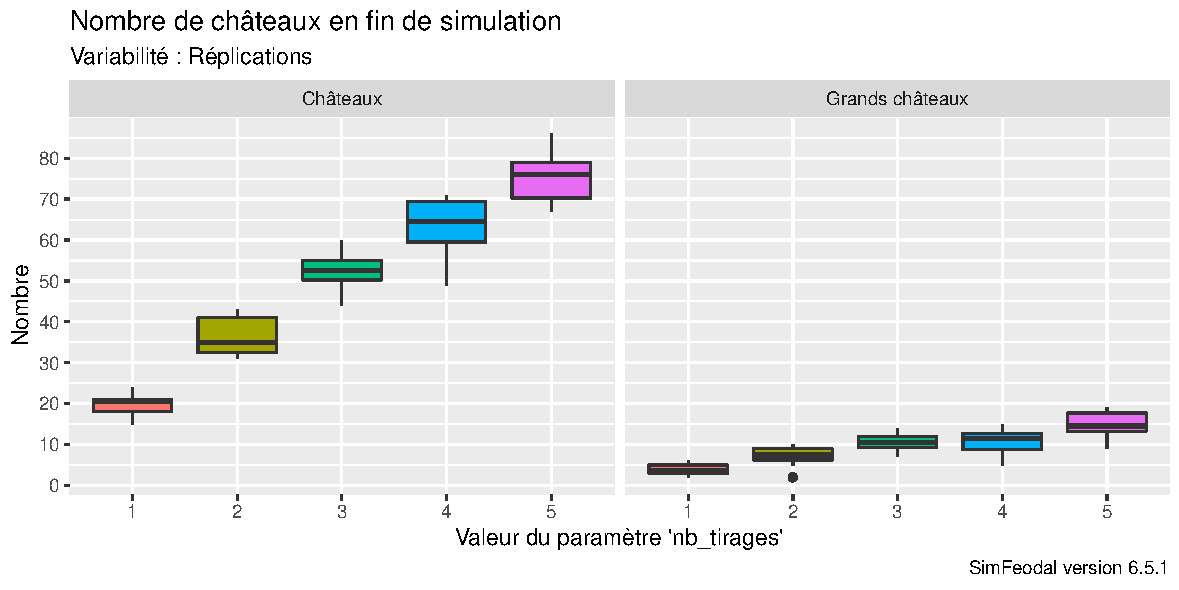
\includegraphics[width=\linewidth]{img/calibrage_nombre_chateaux.pdf}
	\caption[Influence du paramètre \textsf{nb\_tirages} sur le nombre de châteaux.]{Influence du paramètre \textsf{nb\_tirages} sur le nombre de châteaux%\footnotemark.
	}
	\label{fig:calibrage-param-chateaux}
\end{figure}
%\footnotetext{
%	Ce graphique représente une version légèrement différente de la 6.5.1 présentée dans le reste du chapitre.
%	Certaines valeurs de paramètres y sont adaptées au calibrage, fin, des effets de contexte liés aux châteaux.
%}

En jouant sur les différents paramètres associés à la construction d'un château, on obtient un ensemble de valeurs de paramètres qui amènent à la construction d'une quantité régulière de châteaux, dont le nombre en fin de simulation correspond aux données empiriques (\cref{fig:calibrage-chateaux-nb}).

\begin{figure}[H]
	\centering
	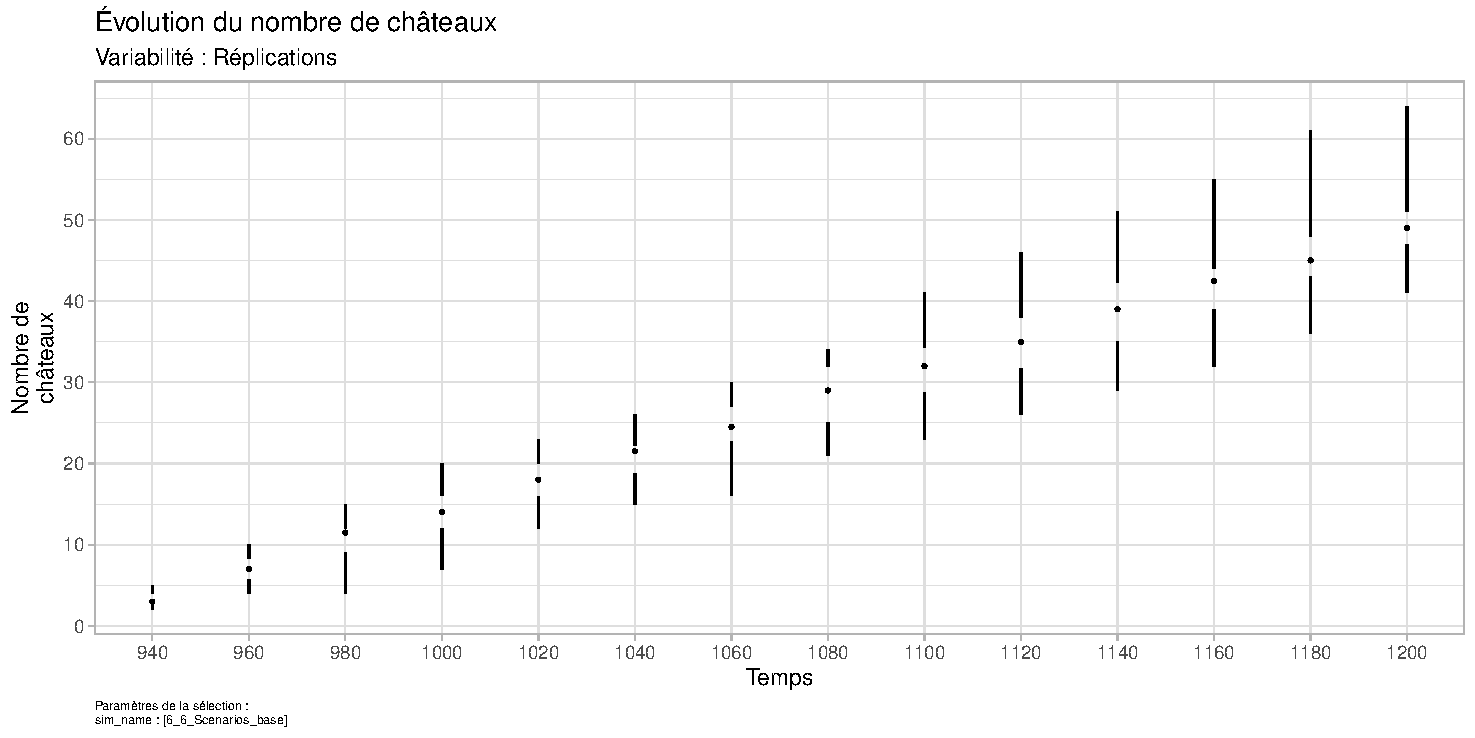
\includegraphics[width=\linewidth]{img/results_6_6/Chateaux_Nb_Haut.pdf}
	\caption{Évolution du nombre de châteaux simulé par le modèle calibré. %Version 6.6 de SimFeodal.
	}
	\label{fig:calibrage-chateaux-nb}
\end{figure}

\paragraph{Détail des types des châteaux}

Le nombre de châteaux n'est toutefois pas la seule valeur empirique sur laquelle on essaie d'ajuster le contexte.
En effet, dans SimFeodal, on distingue plusieurs catégories de châteaux, d'une part selon leur importance (gros et petits châteaux), et d'autre part selon le type de seigneurs qui les ont construits (petits ou grands seigneurs).
L'importance des châteaux joue sur leur attractivité vis-à-vis des foyers paysans (un gros château contribue davantage à l'attractivité du pôle d'attraction qui le contient qu'un petit château).
Le type de propriétaire joue quant à lui sur le prélèvement des droits associés : un château construit par un grand seigneur a des zones de prélèvement associées plus larges que celles d'un petit seigneur.

Ces distinctions dans le modèle, d'un niveau de détail supérieur à celui de nombreux mécanismes, sont possibles car elles s'appuient sur des typologies empiriques connues sur la région d'étude.
Leur prise en compte permet d'affiner le contexte spatial dans lequel les foyers paysans évoluent, aussi bien en matière de répulsion (\textit{push}, par le type de constructeur) que d'attraction (\textit{pull}, par les attractivités différenciées).


À la fin de la période, en Touraine, on estime à une dizaine le nombre de \og forteresses\fg{}\footnote{
	Trouver ref. avec Samuel pour distinguer les \og forteresses importantes\fg{} et les \og points fortifiés secondaires\fg{}
}.
Dans SimFeodal, on a donc pu calibrer les paramètres liés à la promotion de châteaux de manière à obtenir 10 gros châteaux (correspondants aux forteresses empiriques) et 40 (50 - 10) petits châteaux en fin de simulation.

On connaît de plus, empiriquement, les seigneurs à l'initiative de la construction des châteaux.
Dans la plupart des cas (de 40 à 45 châteaux sur les 50), ce sont les seigneurs les plus importants : ducs et comtes d'Anjou et de Touraine, représentés dans SimFeodal par les grands seigneurs.
Les 5 à 10 châteaux restant sont issus de seigneurs de moindre importance qui ont toutefois acquis une puissance symbolique et militaire bien supérieure à celles des autres petits seigneurs.
Dans SimFeodal, on a donc calibré les paramètres régissant les mécanismes de création de châteaux, différenciés pour les grands et petits seigneurs, afin que les valeurs obtenues par simulation soient similaires aux valeurs empiriquement connues.

Les graphiques de la \cref{fig:calibrage-chateaux-composition} présentent les résultats obtenus dans la dernière version de SimFeodal.
Ils ne sont pas entièrement satisfaisants, mais résultent d'un compromis entre le calibrage des trois indicateurs que sont le nombre et le type des châteaux, ainsi que le statut de leurs constructeurs.

\begin{figure}[H]
	\centering
	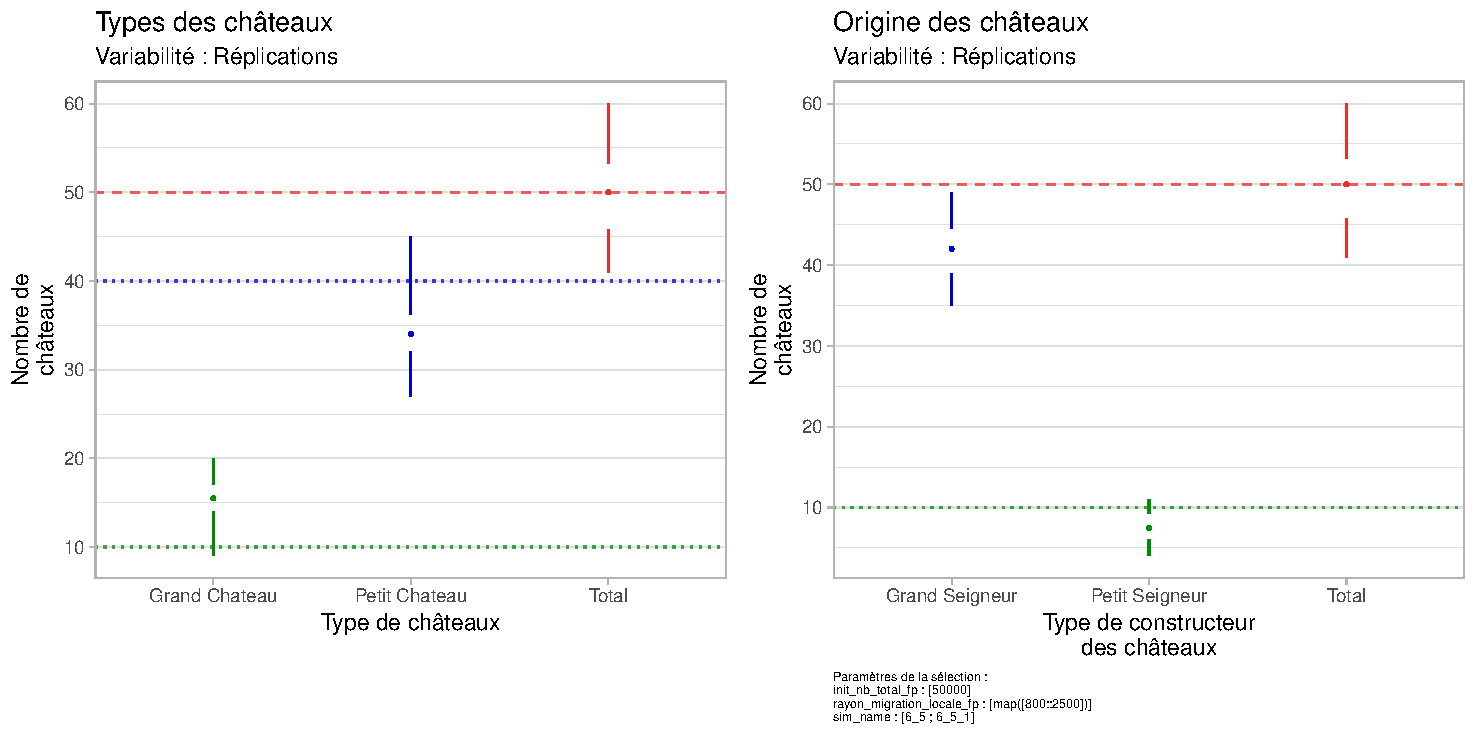
\includegraphics[width=\linewidth]{img/Chateaux_Types_condenses.pdf}
	\caption{Détail de la composition des châteaux en fin de simulation à l'issu du calibrage de SimFeodal.\\
	\textit{Les lignes horizontales en pointillés représentent les objectifs à atteindre, définis selon les connaissances empiriques.}}
	\label{fig:calibrage-chateaux-composition}
\end{figure}


\clearpage
\subsection{Résultats des simulations}

\begin{tcolorbox}[breakable,left=0pt,right=0pt,top=0pt,bottom=0pt,
	colback=yellow!50,colframe=black,width=\dimexpr\textwidth\relax, 
	enlarge left by=0mm, boxsep=5pt,arc=0pt,outer arc=0pt]
Il manque des corrections de Lena, depuis cette intro jusqu'à la figure 6.6 (nombre de pôles et part des agrégats comprenant un pôle).
Lui redemander la version numérique de sa correction, que je n'ai pas eu pour ce petit bout.
\end{tcolorbox}



Nous avons largement décrit, dans le \hl{chapitre 3}, les objectifs poursuivis par le modèle et les indicateurs de sortie de simulation employés pour les évaluer.
Pour rappel, ces objectifs peuvent être catégorisés en trois familles, selon les objectifs thématiques qu'ils cherchent à reproduire : 
\begin{itemize}
	\item Polarisation du système de peuplement : le modèle parvient-il à faire émerger une structure polarisée et concentrée de l'habitat, où les foyers paysans sont concentrés dans des agrégats de population plutôt que dispersés comme dans la situation initiale ?
	\item Hiérarchisation du système de peuplement : depuis une situation initiale composée d'une faible hiérarchie dans les agrégats (des \og agglomérations secondaires antiques\fg{} d'une trentaine de foyers et des \og villages\fg{} d'une dizaine de foyers), parvient-on à une structure hiérarchique, proche du modèle log-normal identifié dans la majorité des systèmes de peuplement historiques et contemporains ?
	\item Fixation et dissémination du peuplement : on estime que la population, initialement assez mobile (relativement à la granularité temporelle du modèle, soit tous les 20 ans) tend peu à peu à se fixer.
	Cette fixation, dans des agrégats, s'assortit d'une dispersion à l'échelle de la région modélisée : d'une occupation dispersée et quasi-aléatoire, l'objectif thématique est que les agrégats maillent progressivement l'ensemble du monde simulé.
	Observe-t-on bien ces deux processus dans le déroulement des simulations ?
\end{itemize}

Dans cette partie, nous allons synthétiquement commenter les indicateurs de sortie de simulation issus de la version calibrée (6.6) de SimFeodal, en analysant l'écart entre les objectifs attendus, thématiques, et les résultats du modèle.

\begin{mdframed}[backgroundcolor=black!5,footnoteinside=false]
Par soucis de parcimonie et de synthèse, les résultats présentés par la suite ne sont qu'une sélection de l'ensemble des résultats du modèle.
Nous invitons le lecteur à les consulter directement dans l'application SimEDB d'où ces indicateurs sont extraits.
Le lien suivant permet d'accéder aux résultats spécifiques à la version présentée ici : \hl{LIEN direct}
\end{mdframed}

\subsubsection{Résumé global des résultats \label{ssec:results-global}}

Avant de chercher à analyser les résultats du modèle à une échelle fine, le \cref{tab:results-basique} peut déjà synthétiser une bonne part des résultats agrégés, en fin de simulation.
Il rassemble les indicateurs de sortie de simulation quantitatifs, qui décrivent uniquement l'état du modèle en 1200, à la fin de la simulation.


\begin{table}[H]
	\captionsetup{singlelinecheck=off}
	\centering
	\small
	{\renewcommand{\arraystretch}{1.3}%
	\begin{tabular}{|p{3cm}|p{2.2cm}|p{1.5cm}|p{1.5cm}|p{1.5cm}|p{1.5cm}|p{1.5cm}|}
		\hline
		\textbf{Indicateur} & \textbf{Valeur} \textbf{attendue}\footnotemark & \textbf{Moyenne} & \textbf{Médiane} & \textbf{Q1} & \textbf{Q3} & \textbf{Écart-type} \\ \hline
		\textit{Agrégats} & \textit{200} & 249 & 248 & 244 & 253 & 10.45 \\ \hline
		\rowcolor[HTML]{DCDCDC} \textit{Châteaux} & \textit{50} & 49 & 49 & 47 & 51 & 5.82 \\ \hline
		\textit{Gros châteaux} & \textit{10} & 15 & 15 & 13 & 17 & 2.87 \\ \hline
		\rowcolor[HTML]{DCDCDC} \textit{Seigneurs} & \textit{200} & 198 & 196 & 191 & 204 & 8.79 \\ \hline
		\textit{Églises paroissiales} & \textit{300} & 348 & 348 & 338 & 359 & 12.96 \\ \hline
		\textit{Distance moyenne entre églises} & \textit{3 000 m} & 1 459 m & 1 456 m & 1 391 m & 1 537 m & 97 m \\ \hline
		\textit{Part de foyers paysans isolés} & \textit{20 \%} & 30 \% & 30 \% & 30 \% & 30 \% & 0.8 \% \\ \hline
		\textit{Augmentation de la charge fiscale des foyers paysans} & \textit{x 3} & x 2.4 & x 2.4 & x 2.4 & x 2.5 & x 0.03 \\ \hline
		\rowcolor[HTML]{DCDCDC} \textit{Nombre de Foyers Paysans} & \multicolumn{1}{c|}{---} & 40 000 & 40 000 & 40 000 & 40 000 & 0 \\ \hline
		\rowcolor[HTML]{DCDCDC} \textit{Densité de population} & \multicolumn{1}{c|}{---} & 6.25 & 6.25 & 6.25 & 6.25 & 0 \\ \hline
	\end{tabular}}
	\caption[Indicateurs numériques de la version 6.6 de SimFeodal.]{
		Indicateurs numériques de la version 6.6 de SimFeodal.\\
		Valeurs de paramètres :~\vspace{-.3em}
		\begin{itemize}
		  \setlength{\itemsep}{-14pt}
		\item \textsf{sim\_name : 6.6}\\
		\item \textsf{croissance\_demo = 0} \&
		\textsf{init\_nb\_total\_fp = 40000} \\
		\item \textsf{rayon\_migration\_locale\_fp = map([800::2500])}
		\end{itemize}
	}
	\label{tab:results-basique}
\end{table}
\footnotetext{Objectif en fin de simulation}

On y constate en premier lieu que les ordres de grandeur sont plutôt respectés, à l'exception peut-être de la distance entre églises paroissiales\footnote{
	La distance moyenne simulée	est ainsi de 1459m, c'est-à-dire deux fois moindre que les estimations empiriques.
	Notons que cela s'explique notamment par le nombre trop élevé d'églises paroissiales, et par la difficile constitution de cet indicateur : les données empiriques concernent surtout les paroisses rurales, alors que l'on tient ici compte de l'ensemble des églises paroissiales.
	Les églises paroissiales urbaines, très proches les unes des autres, tirent ainsi considérablement la moyenne des distances à la baisse.
	Il est difficile, dans le modèle, de différencier les églises paroissiales rurales et urbaines, et on ne peut donc obtenir un indicateur de sortie directement comparable aux données empiriques.
}.

Concernant les autres indicateurs, on peut noter qu'ils sont un peu trop importants, ce qui est rendu plus significatif par des variabilités faibles (les médianes et quartiles sont assez proches de la moyenne, et l'écart-type est faible relativement aux grandeurs considérées).
Le nombre d'agrégats et d'églises paroissiales simulés dépasse ainsi dans les deux cas d'une cinquantaine les valeurs empiriques correspondantes.
La part de foyers paysans isolés en fin de simulation est trop importante de 10\%, quand bien même l'intervalle de confiance empirique est assez flou.

Le nombre de gros châteaux dépasse significativement l'objectif, comme on a pu le constater dans la \cref{fig:calibrage-chateaux-composition} (gauche), mais on expliquait alors que nous ne parvenions à ajuster davantage cette valeur aux quantités empiriques sans déstabiliser d'autres éléments du modèle.

Le dernier indicateur, l'augmentation de la charge fiscale des foyers paysans, est quant à lui assez satisfaisant : il est certes plus faible que l'objectif empirique fixé (augmentation de 2.4 au lieu de 3 de la charge fiscale moyenne entre le début et la fin de la simulation), mais dans le cas de cet objectif empirique difficile à estimer, cette valeur nous paraît suffisante.

Dans la suite de cette partie, nous menons une analyse plus fine des résultats du modèle, en observant de manière plus précise les valeurs des indicateurs de sortie de simulation qui caractérisent les \og trois familles\fg{} d'objectifs thématiques : polarisation, hiérarchisation et fixation-dissémination.

\subsubsection{Capacité du modèle à simuler la polarisation des foyers paysans}

Les résultats mettent en évidence une forte concentration des foyers paysans, dont la part de foyers isolés diminue de manière importante, d'environ 90\% à 30\% en fin de simulation (\cref{fig:results-concentration-fp}).

\begin{figure}[H]
	\centering
	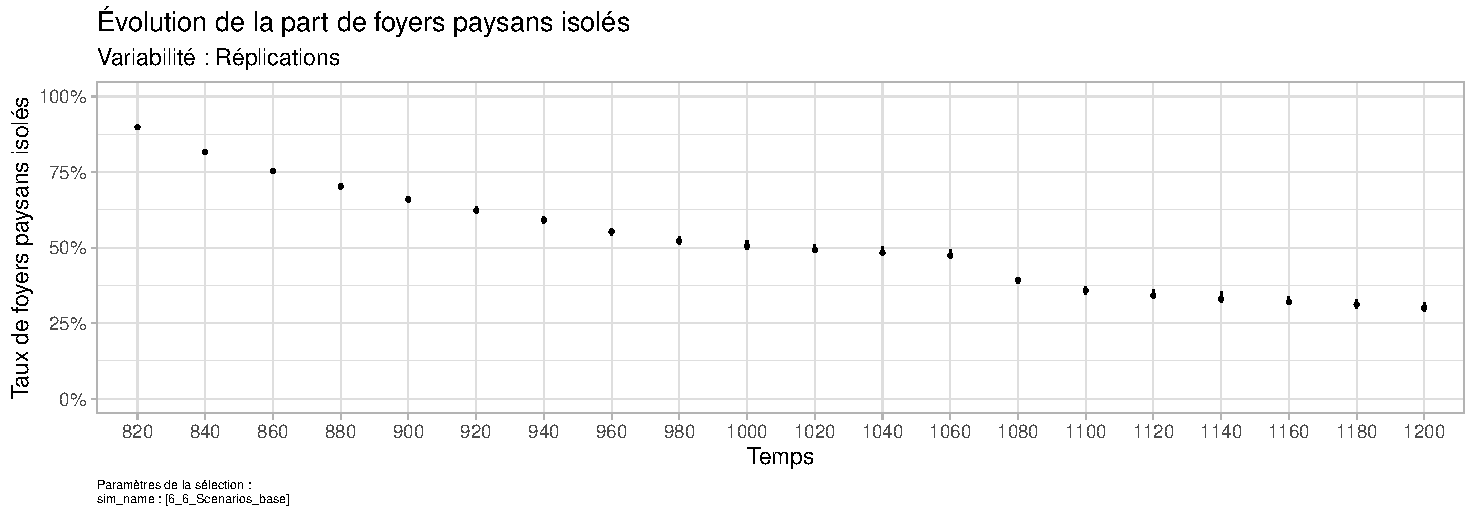
\includegraphics[width=\linewidth]{img/results_6_6/FP_Concentration_Haut.pdf}
	\caption{Concentration des foyers paysans.}
	\label{fig:results-concentration-fp}
\end{figure}

Cette diminution paraît assez régulière, en dépit d'une légère rupture de tendance entre 1060 et 1080, période qui correspond dans le modèle à une évolution du seuil de satisfaction religieuse.
Notons que parmi les 20 réplications étudiées, cet indicateur se montre extrêmement stable, les marques visuelles de variabilité étant à peine visibles.

\begin{figure}[H]
	\centering
	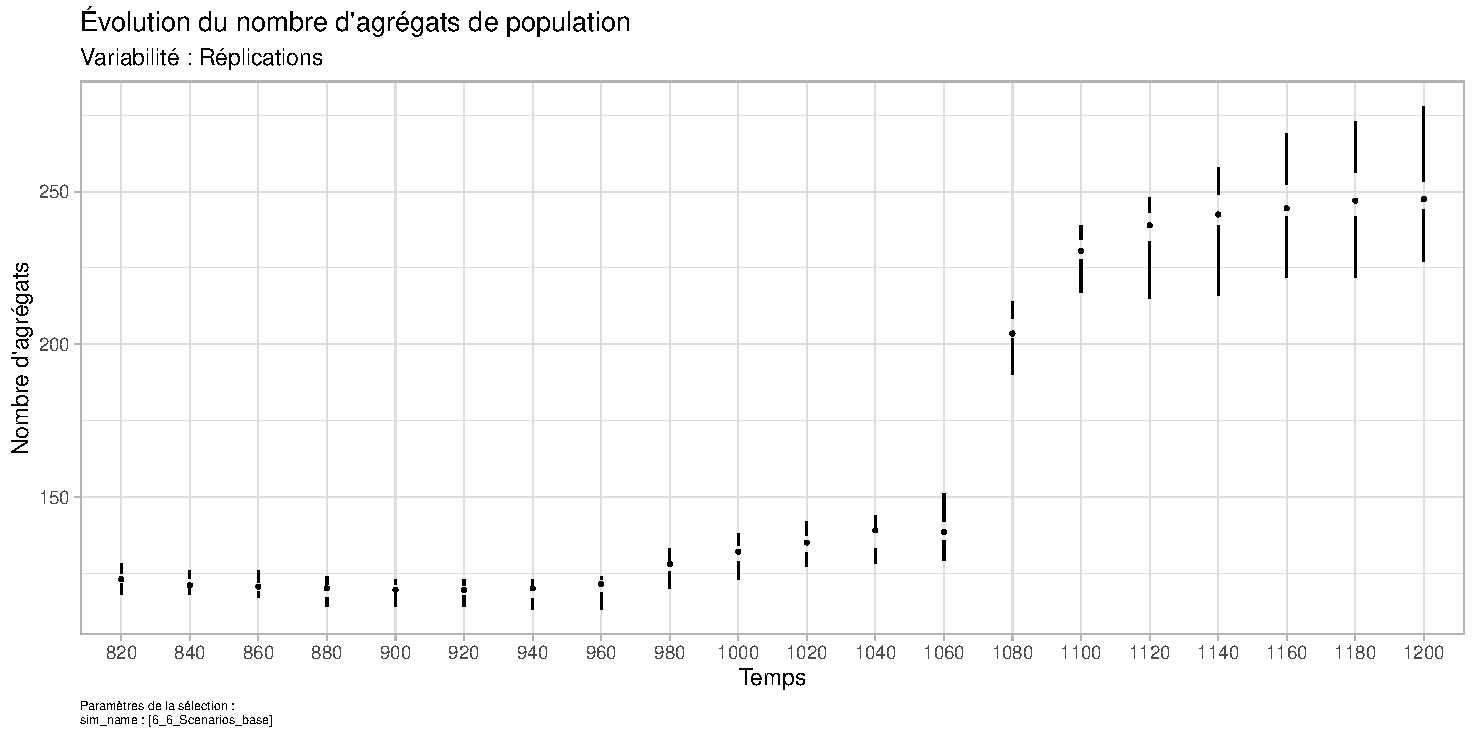
\includegraphics[width=\linewidth]{img/results_6_6/Agregats_Nb_Haut.pdf}
	\caption{Nombre d'agrégats.}
	\label{fig:results-nb-agregrats}
\end{figure}

La concentration des foyers paysans s'effectue à destination d'un nombre croissant d'agrégats (\cref{fig:results-nb-agregrats}).
Dans l'évolution de ce nombre, on constate un effet de seuil important entre 1060 et 1080 (pour les mêmes raisons que l'augmentation de la concentration), mais aussi, un premier changement de tendance entre 940 et 960 d'ampleur moindre.
Ces deux paliers caractérisent les trois régimes repérés empiriquement, c'est-à-dire une augmentation lente, suivie d'une augmentation rapide et enfin une stabilisation du nombre d'agrégats.

À la différence d'une simple concentration du peuplement, la polarisation implique que des éléments (des pôles) jouent un rôle d'attracteur, et que la concentration s'effectue donc à proximité de ces pôles.

Dans SimFeodal, on cherche donc d'une part à ce que les foyers paysans se concentrent et forment des agrégats, et d'autre part à ce que ces agrégats se constituent autour des pôles d'attraction constitués par les agents attracteurs du modèle (églises paroissiales, châteaux et agrégats dotés de communautés paysannes).
Pour savoir si le modèle parvient bien à reproduire le fait stylisé qu'est la polarisation du peuplement, on mobilise donc des indicateurs relatifs à la quantité de pôles et à leur localisation.

Dans cette version du modèle, on constate bien une croissance du nombre de pôles (\cref{fig:results-nb-poles-agregats}-a), assez semblable à celle des agrégats en termes de rythme et de valeurs.
Les valeurs atteintes (environ 250 pôles en fin de simulation) sont très satisfaisantes, particulièrement au regard des résultats de la version 0 du modèle (\hl{ref chap 3 ou annexe}).

\begin{figure}[H]
	\centering
	\hspace{5pt}
	\subfloat[~]{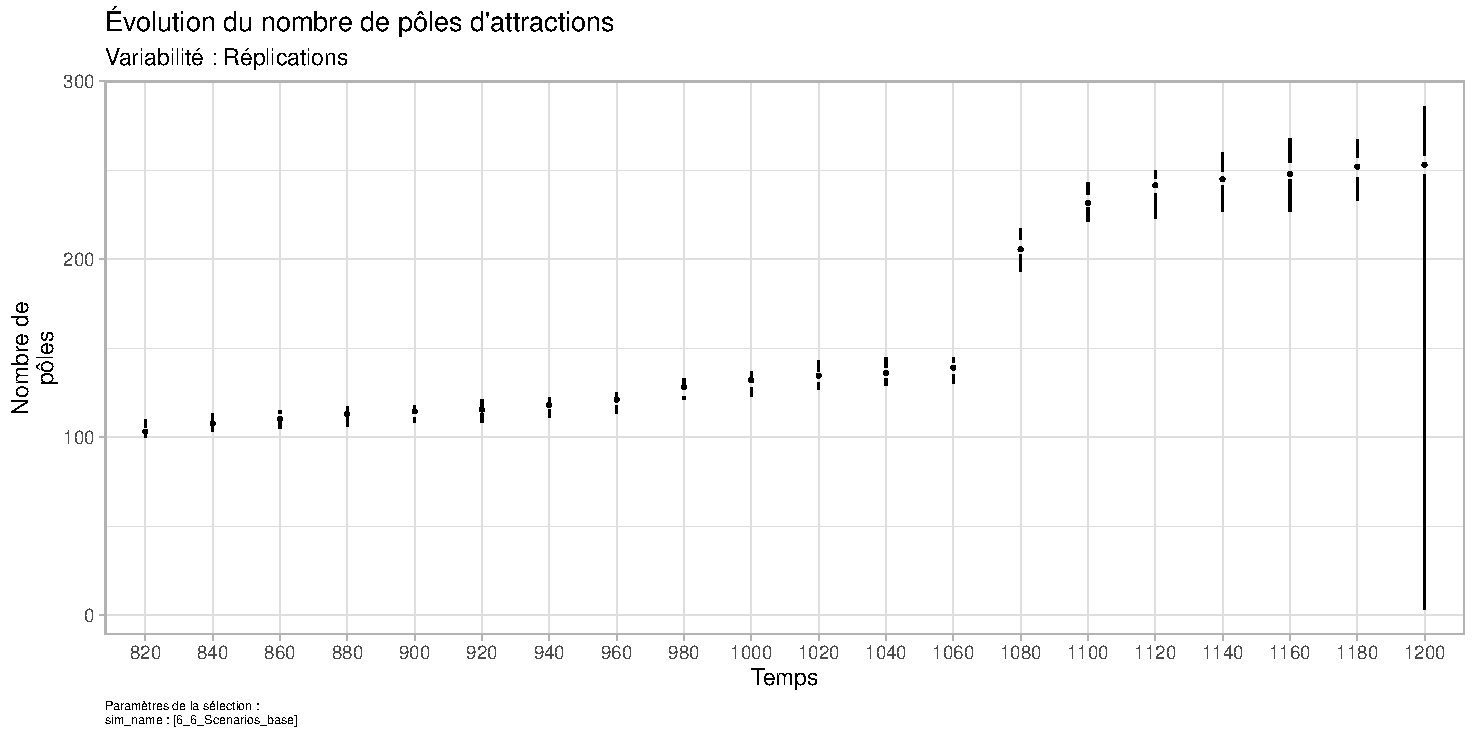
\includegraphics[width=.49\linewidth]{img/results_6_6/Poles_Nb_Haut.pdf}}
	\subfloat[~]{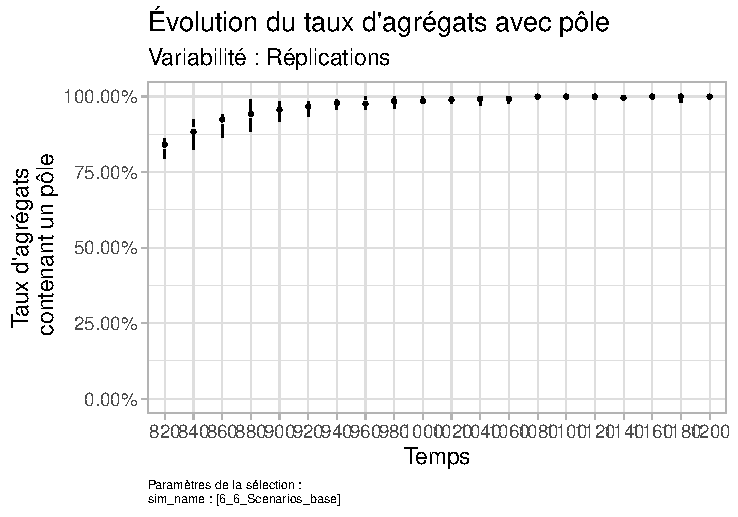
\includegraphics[width=.49\linewidth]{img/results_6_6/Agregats_Poles_Haut.pdf}}
	\caption[Nombre de pôles et part des agrégats comprenant un pôle.]{Nombre de pôles et part des agrégats comprenant un pôle.}
	\label{fig:results-nb-poles-agregats}
\end{figure}

La \cref{fig:results-nb-poles-agregats}-b présente elle-aussi des résultats satisfaisants, qui viennent préciser l'analyse précédente.
Cette figure présente l'évolution du taux d'agrégats qui sont situés dans un pôle d'attraction.
On remarque que ce taux augmente très rapidement pour ensuite se maintenir autour de 100\% : cela signifie que tous les agrégats sont situés dans un pôle, et donc que les agrégats se sont bien formés autour de pôles d'attraction plutôt que de manière purement dispersée.
Cette figure constitue ainsi un des indices montrant que SimFeodal parvient bien à reproduire le processus de polarisation tel qu'observé empiriquement.

Les cartes de la \cref{fig:results-carte-agregats_poles} permettent de noter que le semis des pôles se confond spatialement avec celui des agrégats, ce qui amène un élément d'interprétation supplémentaire : les agrégats sont bien constitués dans des pôles (paragraphe précédent), mais en plus, tous les pôles semblent contenir un ou des agrégats.
Le modèle fait donc émerger une quasi-équivalence entre pôles et agrégats, quasi-équivalence que l'on retrouve chez \textcite[27-28]{le1976eglise}, en assimilant les pôles à leurs seules églises : \og Le village appelle l'église. [...] L'église fait naître le village.\fg{}.
\hl{Retrouver dicton autour de \og pas d'église sans village, pas de village sans église\fg{}.}

%Ces agrégats et les pôles correspondant sont bien plus dispersés dans l'espace du modèle que dans la version 0, et on constate, au moins visuellement, que le semis des pôles se confond avec celui des agrégats (\cref{fig:results-carte-agregats_poles}).
%Sur ces cartes, on constate une occupation importante de l'espace, largement due à une population bien supérieure en version 6.6 (40 000 foyers paysans, contre 4 000 en version 0), mais on remarque toutefois sur la troisième carte, lissée, qu'en dépit d'un semis visiblement homogène, des zones de plus forte densité sont présentes.

\begin{figure}[H]
	\centering
	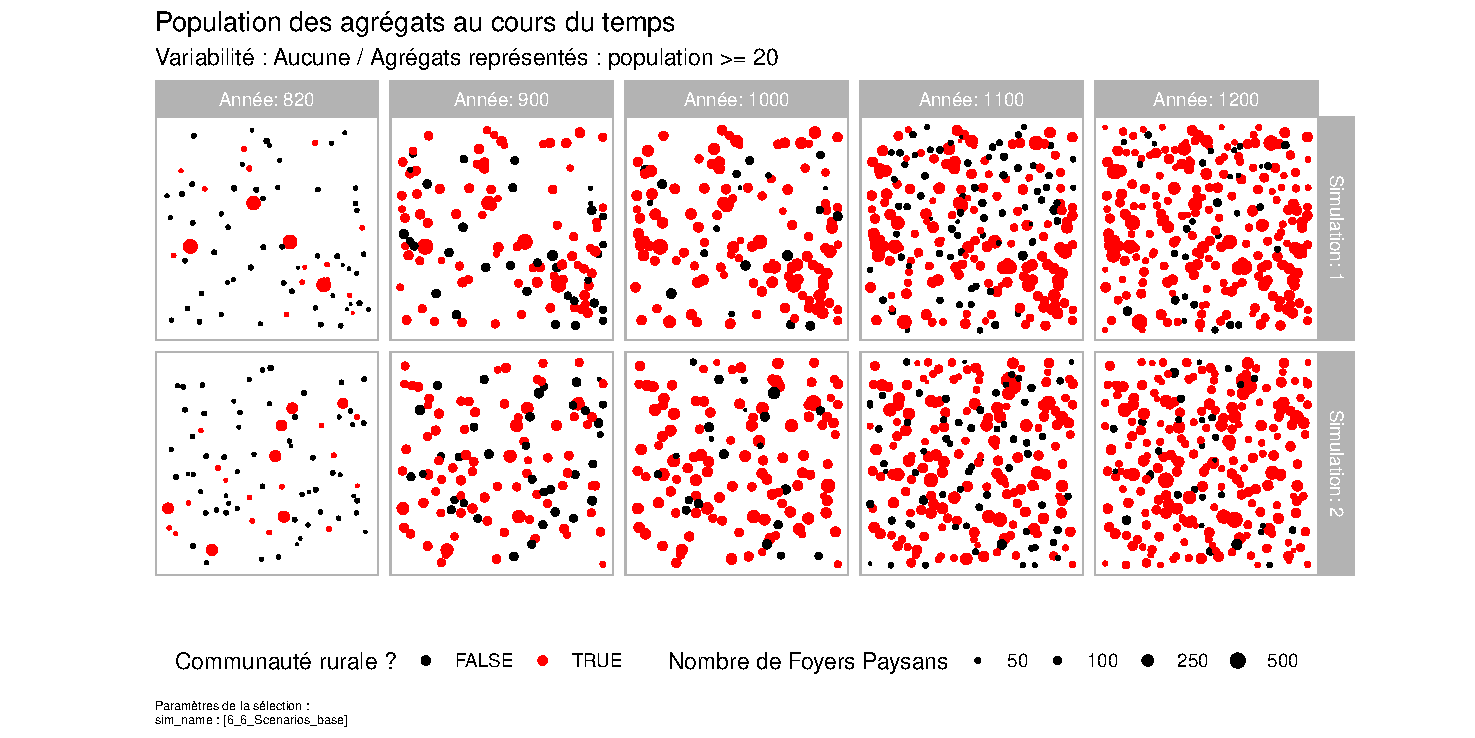
\includegraphics[width=\linewidth]{img/results_6_6/Agregats_Carte_Haut.pdf}
	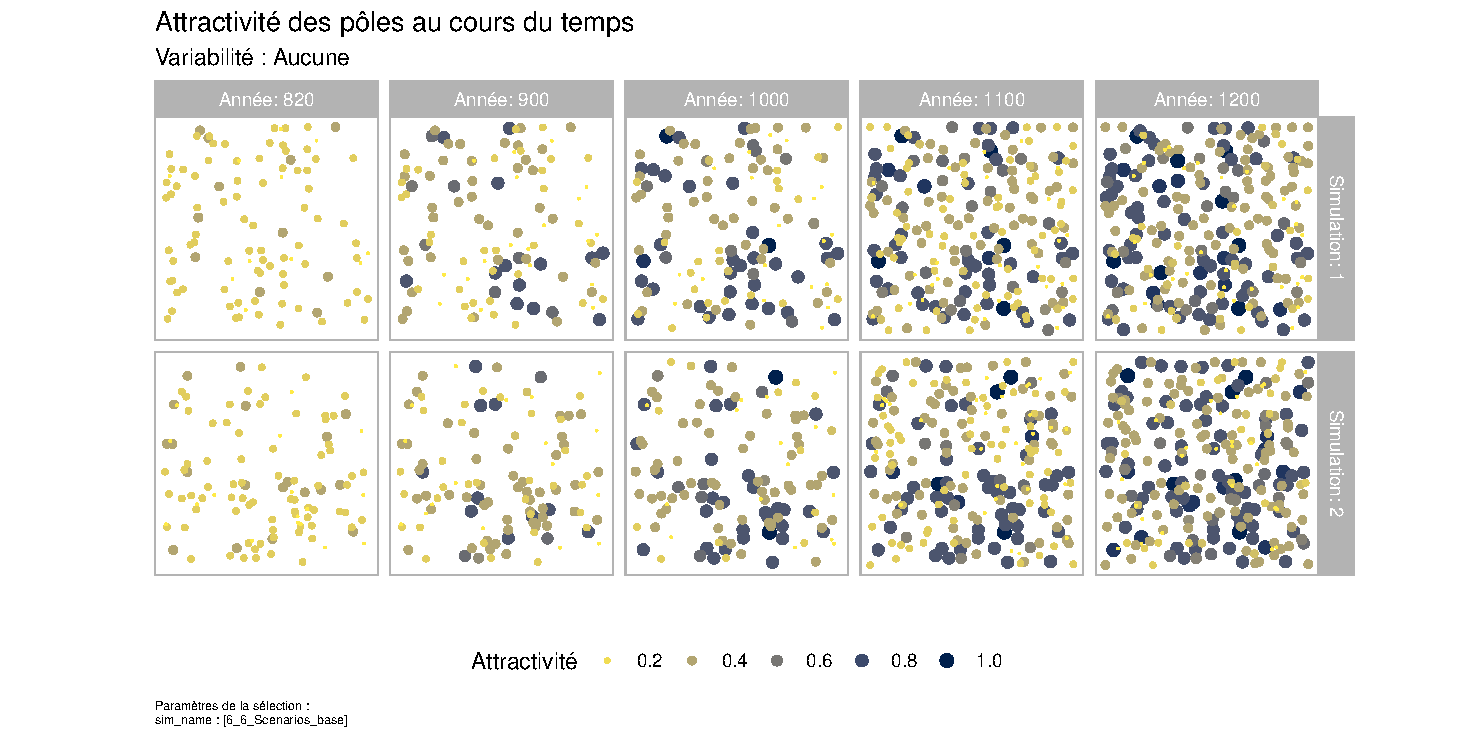
\includegraphics[width=\linewidth]{img/results_6_6/Poles_Carte_Haut.pdf}
	\caption{Dispersion spatiales des agrégats et pôles.}
	\label{fig:results-carte-agregats_poles}
\end{figure}

\bigskip
\paragraph[Conclusion intermédiaire]{}
Sur le plan de la polarisation d'ensemble des foyers paysans au sein d'agrégats de population, les résultats du modèle montrent que SimFeodal est entièrement capable de reproduire les attendus.
La valeur finale issue des simulation est certes légèrement inférieure à l'objectif, mais tous les ordres de grandeurs et surtout les rythmes estimés correspondent largement aux estimations issues des connaissances expertes.

\clearpage
\subsubsection{Capacité du modèle à simuler la hiérarchisation du système de peuplement}

Les dernières figures étudiées montraient une forte hétérogénéité dans la taille des agrégats (un agrégat est créé dès 5 foyers paysans, et la légende de la première série de cartes -- dispersion des agrégats-- s'étend entre 50 et 500 foyers), ce qui constitue déjà un indice sur le niveau de hiérarchisation de ces concentrations locales de foyers paysans.

Comme indiqué dans le chapitre 3, il est difficile d'avoir des mesures précises de la distribution statistique attendue dans le système de peuplement.
Les différentes sources historiques divergent aussi bien sur les quantités absolues que sur la forme des distributions.
Ces sources s'accordent en revanche sur une nette hiérarchisation, avec une distribution qui doit tendre vers les formes log-normales dont l'on retrouve l'existence dans les sociétés contemporaines.

%\begin{table}[H]
%	\captionsetup{singlelinecheck=off}
%	\centering
%	\small
%	{\renewcommand{\arraystretch}{1.3}%
%		\begin{tabular}{p{2.5cm}|p{1.5cm}|p{1.5cm}|p{1.5cm}|p{1.5cm}|p{1.5cm}|p{1.5cm}|}
%			\cline{2-7}
%			& \multicolumn{6}{c|}{\textbf{Nombre de foyers paysans}} \\
%			  & \textbf{<100} & \textbf{101-200} & \textbf{201-300} &  \textbf{301-400} &\textbf{ 401-600} & \textbf{>600} \\ \hline
%			 \multicolumn{1}{|c|}{Nombre moyen} & 142 & 78 & 18 & 7 & 4 & 2 \\ \hline
%			 \multicolumn{1}{|c|}{Taux moyen} & 56.8\% & 31.4\% & 7\% & 2.9\% & 1.6\% &<0.1\% \\ \hline
%			 \rowcolor{yellow} \multicolumn{1}{|c|}{\textit{Objectif (taux)}} & \textit{?} & \textit{?} & \textit{?} & \textit{?} & \textit{?} & \textit{?}\\ \hline	
%	\end{tabular}}
%	\caption[Distribution des agrégats par classe de taille en fin de simulation.]{Distribution des agrégats par classe de taille en fin de simulation. \hl{Ne conserver que si Cécile arrive à trouver, pour l'article anglais, une validation des objectifs par EZR/SL.}}
%	\label{tab:distrib-population-agregats}
%\end{table}

\begin{figure}[H]
	\centering
	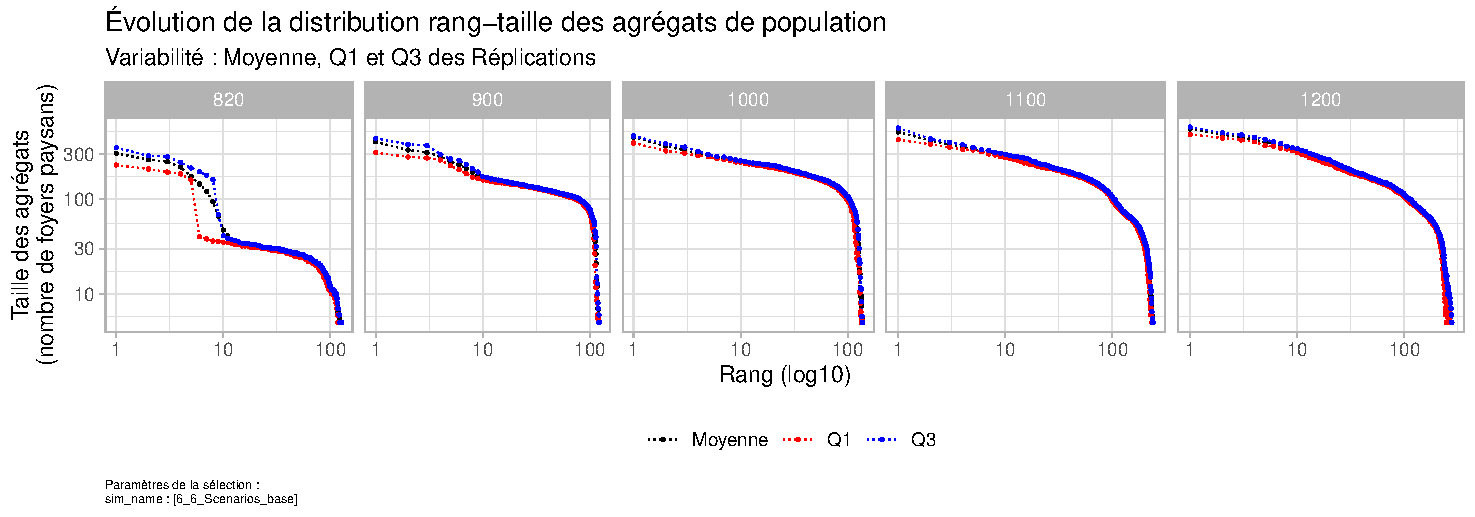
\includegraphics[width=\linewidth]{img/results_6_6/Agregats_RT_Haut.pdf}
	\caption[Hiérarchie des agrégats]{Organisation hiérarchique des agrégats.}
	\label{fig:results-rt-agregats}
\end{figure}

La \cref{fig:results-rt-agregats} montre une claire hiérarchisation des agrégats : la courbe se \og redresse\fg{} au cours de la simulation, marque d'une pente croissante.
Les valeurs absolues augmentent aussi : les plus gros agrégats voient leur population croître.
Le \og coude\fg{} dans la courbe, qui correspond à la longue traîne de petits agrégats, se réduit.
%Contrairement à la version 0 du modèle, la croissance de tous les agrégats semble constante, et on ne remarque pas, visuellement, les tendances à l'éclatement des gros agrégats qui caractérisaient la hiérarchie de cette version.

En parallèle de cette nette hiérarchisation des agrégats, les graphiques de la  \cref{fig:results-rt-poles} permettent de constater une toute aussi nette hiérarchisation des pôles.
Cela n'est pas surprenant dans la mesure où on a vu qu'agrégats et pôles se confondaient, ce qui constitue en soi un résultat satisfaisant.


\begin{figure}[H]
	\centering
	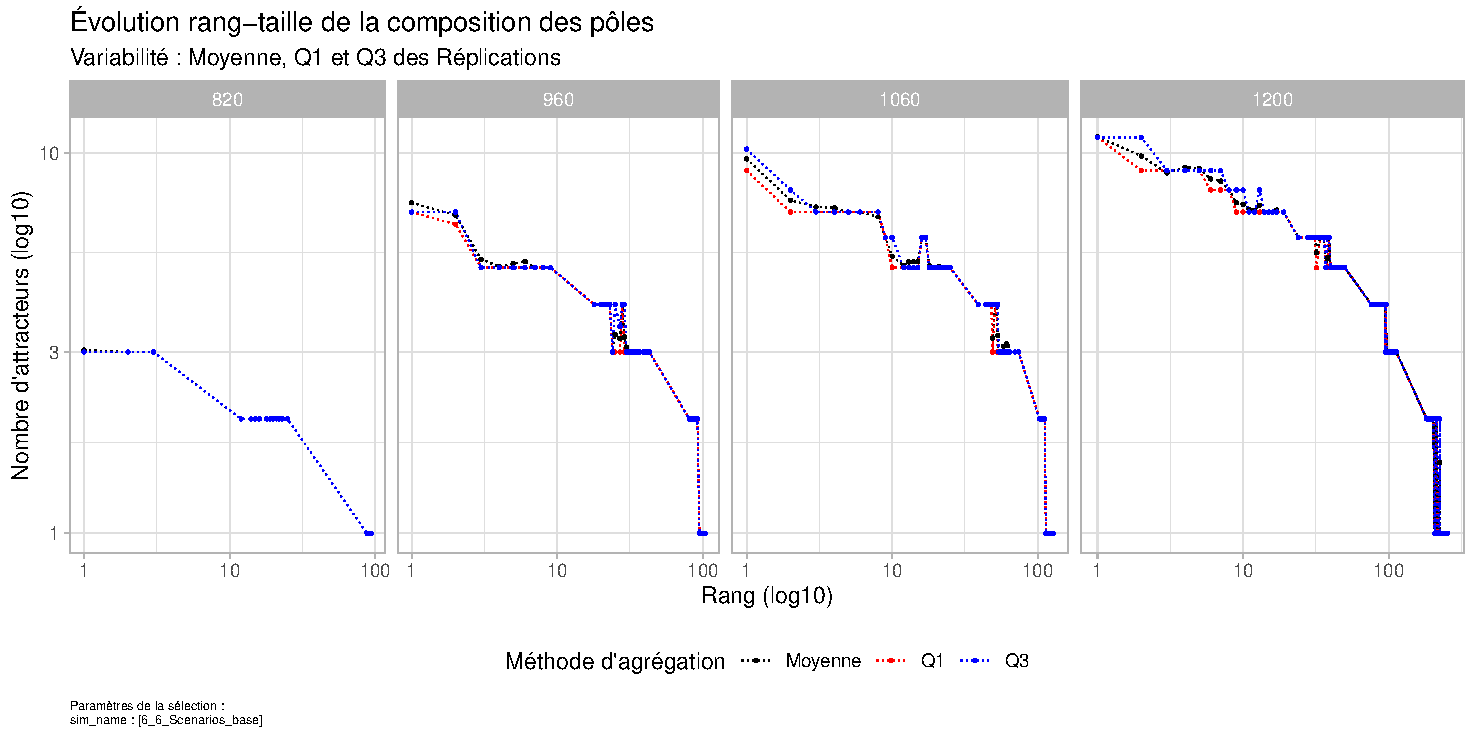
\includegraphics[width=.405\linewidth]{img/results_6_6/Poles_RT_Haut.pdf}
	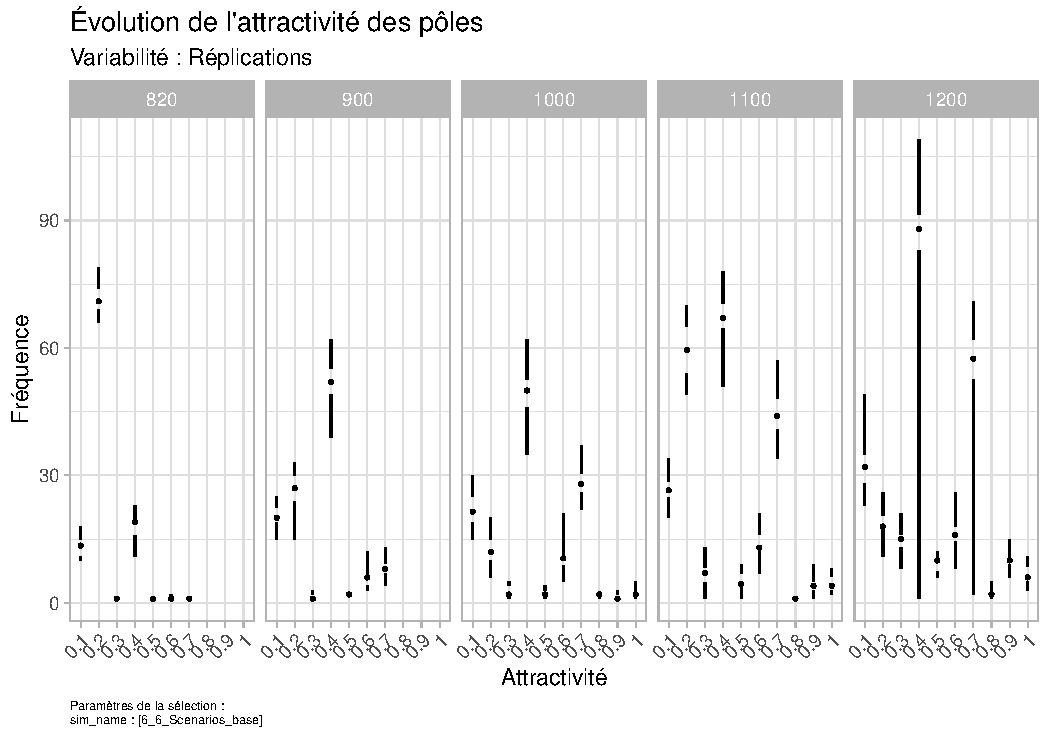
\includegraphics[width=.58\linewidth]{img/results_6_6/Poles_Attrac_Haut.pdf}
	\caption[Hiérarchie des pôles.]{Organisation hiérarchique des pôles.}
	\label{fig:results-rt-poles}
\end{figure}

La mesure représentée dans la figure de gauche -- le nombre d'attracteurs de chaque pôle -- est beaucoup plus \og discrète\fg{} que le nombre de foyers paysans des agrégats.
Il y a moins de modalités (de 1 à une dizaine d'attracteurs, contre de 5 à plus de 500 foyers paysans), donc moins d'effets possibles de coudes.
Ce graphique communique donc plus lisiblement, visuellement, la forte hiérarchisation des pôles.
Comme le nombre maximum d'attracteur augmente régulièrement (environ 3 en début de simulation contre plus de 10 à la fin), on peut dire que dans le modèle, cette hiérarchisation est dûe à une croissance des pôles les plus importants et non à une croissance équitablement répartie.
Par exemple, en fin de simulation, sur les 250 pôles, moins de la moitié est composée de plus de trois attracteurs.

En cela, le modèle reproduit bien l'apparition d'une tête de hiérarchie urbaine, qui trouve une correspondance empirique dans les villes (Amboise, Loches, Chinon\ldots) de la région d'étude, organisées autour de châteaux et composées de multiples églises paroissiales.
La \cref{fig:results-rt-poles}-b montre aussi cette hiérarchisation : elle met en évidence un glissement des modalités d'attraction depuis une valeur de 0.2 (deux églises paroissiales) à un double mode à 0.4 (deux églises et une communauté) et 0.7 (plusieurs églises, un château, une communauté\ldots).


Un dernier élément du modèle en lien avec la hiérarchisation du peuplement est composé par la hiérarchie des paroisses.
On peut extraire deux types de comportements attendus à partir des connaissances empiriques.
\begin{itemize}
	\item En premier lieu, une large majorité des paroisses, que l'on pourrait nommer \og rurales\fg{}, sont peu fréquentées et visent surtout à une desserte équitable de la population.
	Un paroissien ne devait ainsi pas avoir à effectuer plus d'une heure de marche pour se rendre dans son église paroissiale.
	\item En second lieu, les paroisses \og urbaines\fg{} desservent un nombre de paroissiens bien supérieur à celui des paroisses rurales.
	D'après les connaissances expertes, ce nombre reste largement inférieur au millier de paroissiens, puisque de nouvelles paroisses urbaines étaient créées pour décharger les églises paroissiales trop fréquentées.
\end{itemize}
En agrégeant ces types de paroisses, le fait stylisé que l'on cherche à reproduire dans le modèle serait donc d'avoir une distribution composée de deux tendances : une tête de hiérarchie desservant un grand nombre de paroissiens, mais avec une faible hiérarchisation interne (paroisses urbaines), et une très longue traine, cette-fois ci plus hiérarchisée et desservant beaucoup moins de paroissiens (paroisses rurales).


Dans la \cref{fig:results-rt-paroisses}, on constate que le modèle semble reproduire ce type de distribution : on y remarque bien une courbe caractérisée par une double tendance.
Le haut de la hiérarchie présente une pente faible, signe d'une homogénéité importante entre 100 et 300 paroissiens, et est nettement séparé d'une longue traîne, graphiquement presque verticale, inférieure à 100 paroissiens.
Le nombre maximum de paroissiens diminue au cours de la simulation, passant de plus de 1000 à environ 300.

\begin{figure}[H]
	\centering
	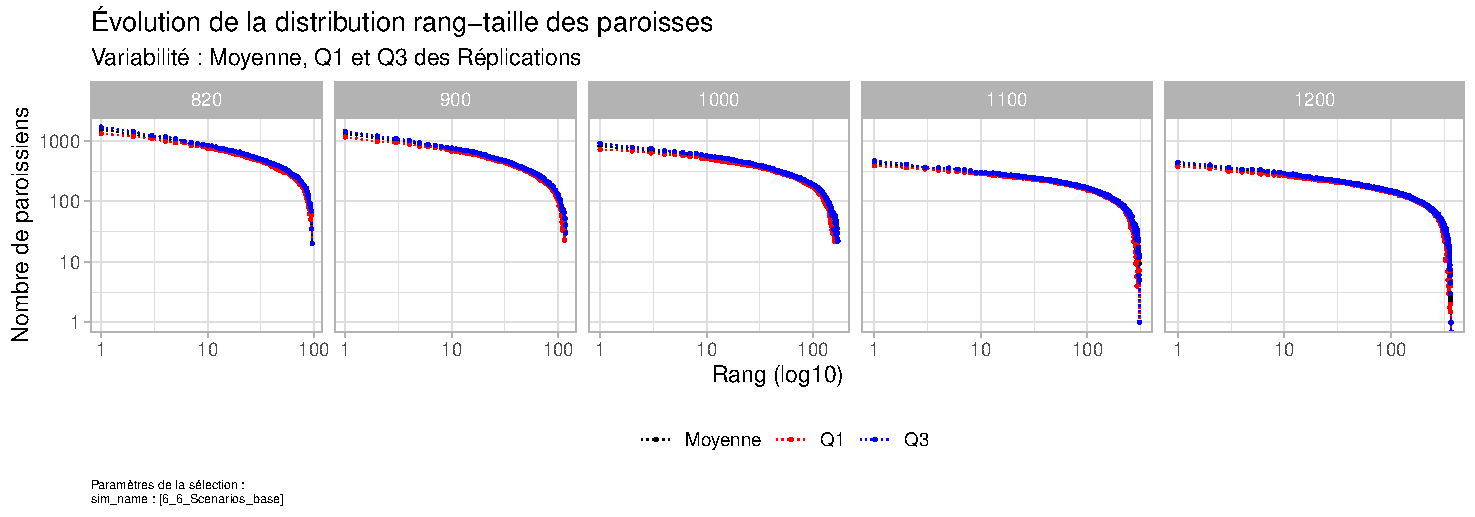
\includegraphics[width=\linewidth]{img/results_6_6/Paroisses_RT_Haut.pdf}
	\caption{Organisation hiérarchique des paroisses.}
	\label{fig:results-rt-paroisses}
\end{figure}

En regardant des indicateurs plus détaillés (\cref{fig:results-paroisses-hierarchie}), on peut remarquer que cela correspond en fait à une forte homogénéisation dans les intervalles de 50 à 200 paroissiens (51-100 et 101-200) qui deviennent en fin de simulation le mode principal de la distribution.
Cet intervalle correspond aux paroisses rurales qui contiennent quelques agrégats ruraux de taille moyenne à faible (\cref{fig:results-rt-agregats}).

\begin{figure}[H]
	\centering
	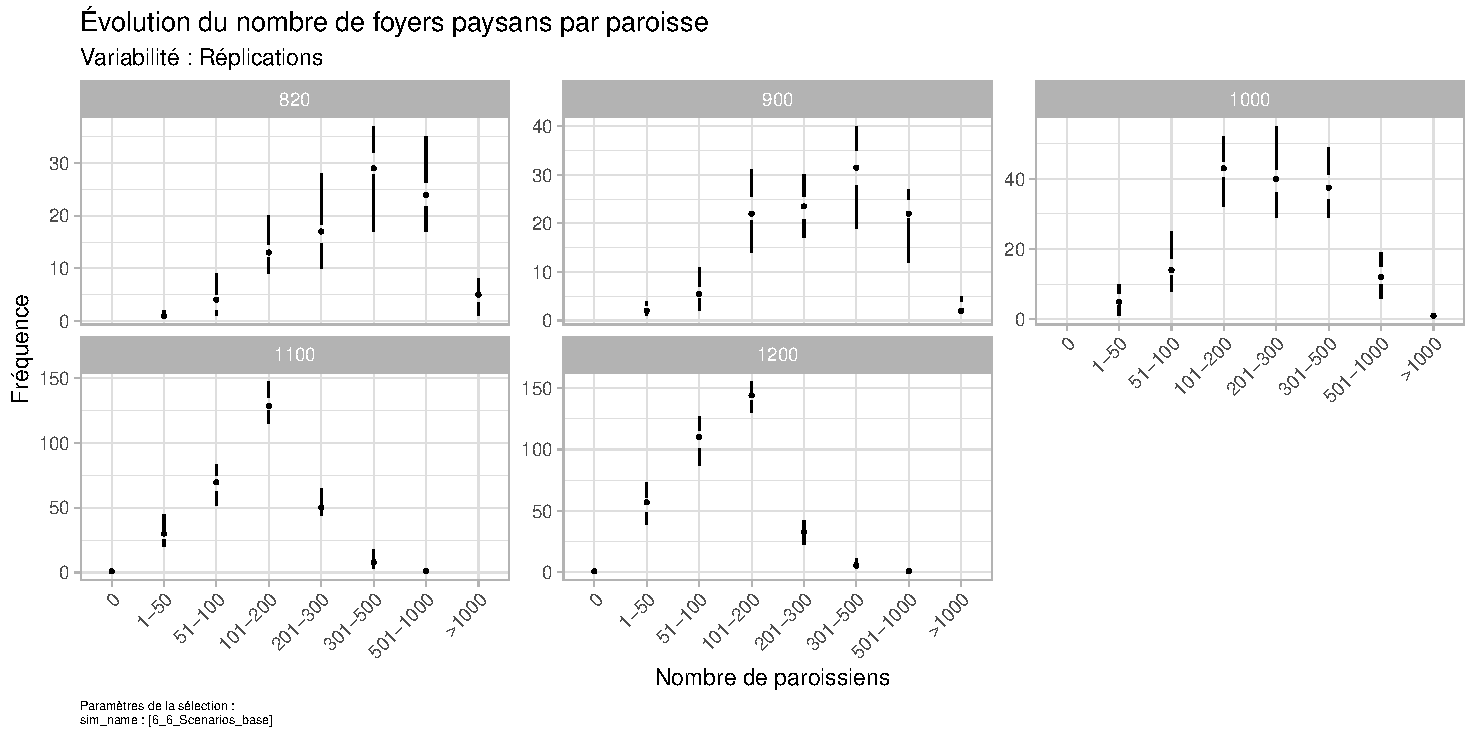
\includegraphics[width=\linewidth]{img/results_6_6/Paroisses_Compo_Haut.pdf}
	\caption{Détail de la distribution hiérarchique des paroisses.}
	\label{fig:results-paroisses-hierarchie}
\end{figure}

SimFeodal parvient donc bien à reproduire la double-densification du maillage paroissial.
En milieu rural, le nombre de paroisses augmente jusqu'à assurer une desserte équitable des foyers paysans qui dans le même temps ont tendance à se concentrer, et en milieu urbain, le nombre de paroisses augmente aussi jusqu'à uniformiser le nombre de foyers paysans par paroisse entre 200 et 300.

\bigskip
\paragraph[Conclusion intermédiaire]{}
Dans l'ensemble, SimFeodal montre une bonne capacité à reproduire la hiérarchisation du système de peuplement.
Avec les informations dont l'on dispose pour évaluer le modèle, on ne peut qu'être satisfait des tendances présentes dans cette version calibrée de SimFeodal.
Le modèle reproduit en effet bien les faits stylisés estimés, même si ces derniers sont formalisés de manière plus floues que par exemple le phénomène de polarisation.
Cette incertitude, ou au moins de manque de détail, est dû à la faiblesse de la documentation empirique sur ces question thématiques : il est déjà difficile d'avoir une estimation des populations à cette période féodale, alors le détail de la forme de distribution de ces populations est une connaissance encore plus dure à estimer.
À ce stade de maturité du modèle, il faudrait sans doute collecter de nouvelles sources historiques pour pouvoir raffiner le comportement du modèle, ou au moins, départager des simulations présentant de légères variations au niveau des indicateurs analysés dans cette sous-partie.

\clearpage
\subsubsection{Capacité du modèle à simuler la fixation et la dissémination du peuplement}

Dans ce dernier objectif thématique, on cherche à vérifier si le modèle parvient bien à reproduire le double processus de fixation des foyers paysans et de dissémination des peuplements dans l'espace.

Dans le modèle, ces processus devraient s'exprimer sous la forme d'un accroissement des migrations (restructuration) suivi d'une diminution nette (fixation).
Àu niveau d'observation des agrégats, on devrait observer une couverture croissante, de plus en plus dense, du monde simulé.

\paragraph{Fixation des foyers paysans}

\begin{figure}[H]
	\centering
	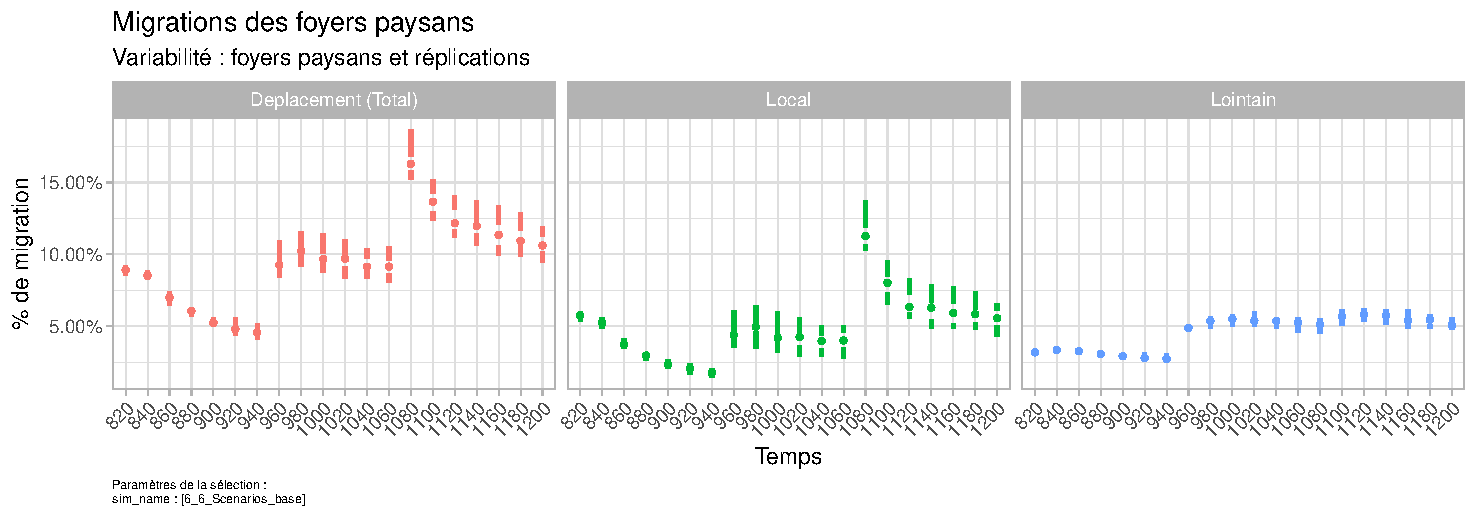
\includegraphics[width=\linewidth]{img/results_6_6/FP_TypeDeplacements_Haut.pdf}
	\caption{Migration des foyers paysans.}
	\label{fig:results-fp-migrations-base}
\end{figure}

La \cref{fig:results-fp-migrations-base} illustre l'évolution des migrations, selon leur type (locale ou lointaine, cf. \hl{chap 2, règles migrations}) au cours du temps.
On y constate que le modèle produit un motif spécifique, composé de trois phases :
\begin{itemize}
	\item Avant 960, les migrations diminuent de manière régulière, depuis près de 10\% de migrations (total) jusqu'à 5\%.
	Dans le modèle, cette période correspond aux premiers regroupements de foyers paysans.
	Ces derniers, initialement isolés, rejoignent des pôles locaux (églises rurales par exemple) et y constituent ainsi de petits agrégats ruraux locaux.
	Ils se fixent dans ces agrégats car il n'y pas encore véritablement de motif d'insatisfaction (religieuse ou de protection du moins).
	\item En 960, deux éléments exogènes viennent perturber le système : l'augmentation de la pression religieuse (diminution des seuils de distance aux églises) et de la pression de protection (nécessité de s'approcher des châteaux).
	En conséquence,le nombre de migrations bondit et retrouve son niveau de début de simulation (environ 10\%).
	Le besoin de protection augmente régulièrement à cette période, et les foyers paysans sont donc sans cesse amenés à migrer, ce qui explique que ce niveau de migration semble stable jusqu'à la fin de cette deuxième phase\footnote{
		Si de nouveaux éléments exogènes ne venaient pas à nouveau perturber le système après 1060, le niveau de migration diminuerait à son tour, comme avant 960.
	}.
	\item Une nouvelle rupture survient en 1060, là encore en raison d'une augmentation, exogène, de la pression religieuse (les seuils acceptables de distance à l'église paroissiale diminuent encore jusqu'à devenir très restreints).
	À nouveau, les migrations (uniquement locales cette fois-ci) augmentent de manière abrupte, et, comme dans la première phase, tendent ensuite à diminuer : le niveau maximal d'exigences (religieuse, de protection) est atteint, et les migrations des foyers paysans y pallient.
\end{itemize}

\begin{figure}[H]
	\centering
	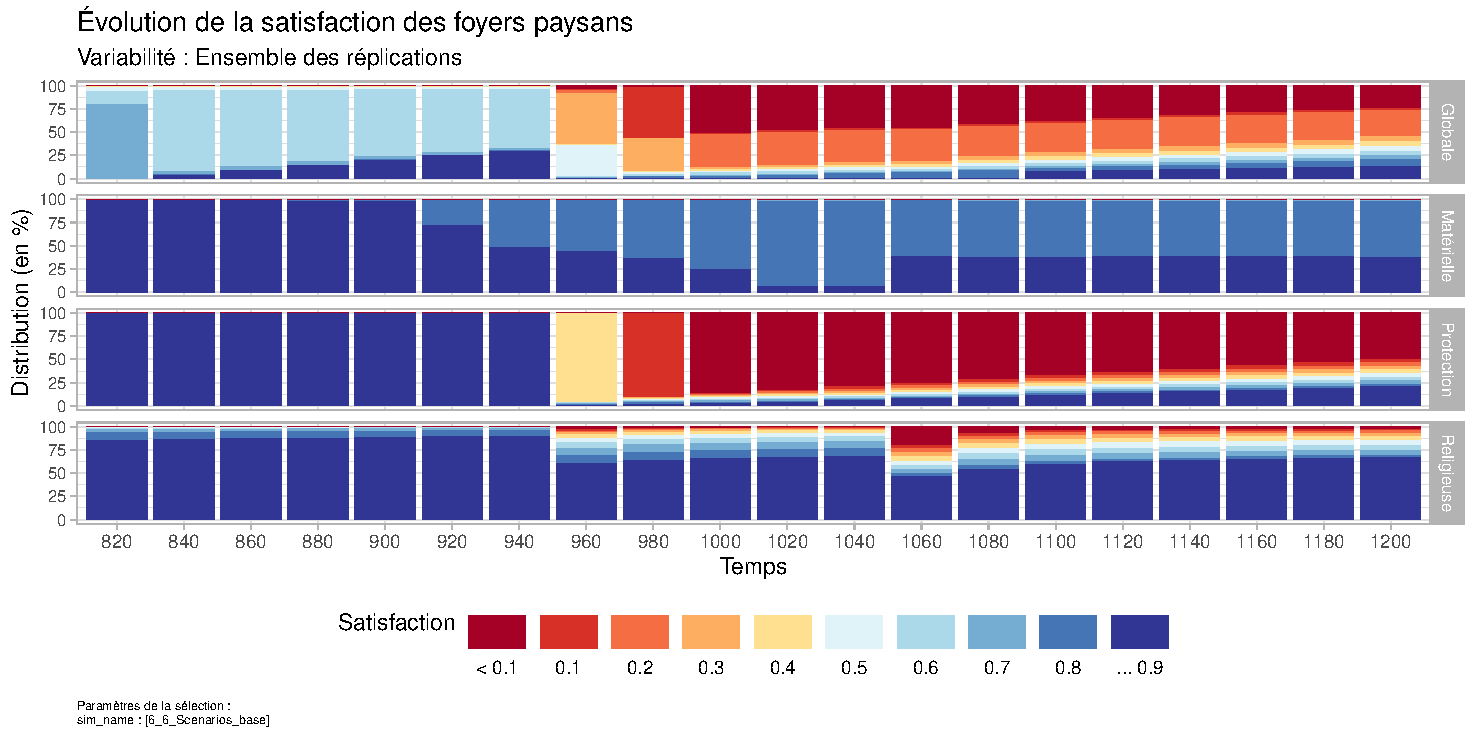
\includegraphics[width=\linewidth]{img/results_6_6/FP_Satisfaction_Haut.pdf}
	\caption{Satisfaction des foyers paysans.}
	\label{fig:results-fp-satisfaction}
\end{figure}

La lecture de la \cref{fig:results-fp-satisfaction}, qui présente les types de satisfaction des foyers paysans au cours de la simulation, vient appuyer cette analyse.
On y retrouve les trois phases observées dans les sorties de simulation.
Avant 960, la satisfaction augmente, et les migrations diminuent avec elle.
En 960, c'est bien la satisfaction de protection qui diminue fortement, poussant les foyers paysans à migrer et déclenchant la seconde phase migratoire.
En 1060, on retrouve le même effet, de moindre ampleur cependant, dans la satisfaction religieuse. À nouveau, les satisfaction diminuent et une nouvelle phase migratoire est initiée.

\begin{figure}[H]
	\centering
	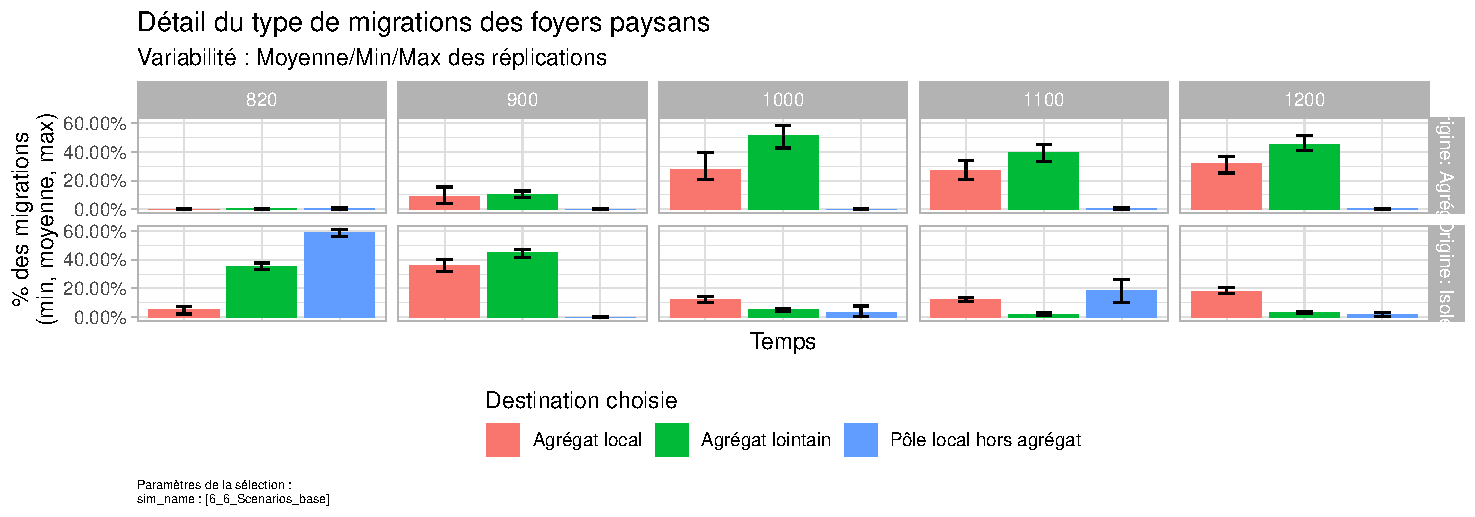
\includegraphics[width=\linewidth]{img/results_6_6/FP_DeplacementsDetail_Haut.pdf}
	\caption{Types de migration des foyers paysans.}
	\label{fig:results-fp-migrations-detail}
\end{figure}

En observant le détail des migrations (\cref{fig:results-fp-migrations-detail}), non continu dans le temps contrairement aux graphiques précédents, on ne retrouve que deux périodes.
La figure nous renseigne toutefois sur une autre dimension liée aux migrations, en fonction ici de l'origine et de la destination des foyers paysans.
On peut alors préciser les observations précédentes : quels foyers paysans migrent, et où ?

En 820 et en 900, la plupart des migrations proviennent de foyers paysans isolés.
Ces migrations, locales et lointaines, permettent aux foyers paysans de rejoindre un agrégat, quel qu'en soit la place dans la hiérarchie.
En 1000 et après, les foyers paysans isolés représentent encore une part substantielle de la population (50\% d'après la \cref{fig:results-concentration-fp}), mais leur poids relatif dans les migrations est devenu bien plus faible que celui des migrations entre agrégats de population.
Après une première période de concentration arrive une période de choix hiérarchique pour les foyers paysans, où les différences d'attractivité des agrégats jouent alors un rôle prépondérant.
Cela indique aussi qu'à partir de cette période, les agrégats sont pour la plupart pérennes et voient alors se mettre une compétition en place.

\paragraph{Dissémination du peuplement}

La répartition des paroisses, dans le modèle, constitue un observable intéressant pour évaluer la dissémination du peuplement.
Comme les paroisses ont comme vocation de desservir la population des foyers paysans, elles constituent un proxy de sa répartition tout au long du temps.
Les indicateurs liés (\cref{fig:results-paroisses-nb,fig:results-paroisses}) donnent une lecture satisfaisante du processus de dissémination.

En premier lieu, on note que le nombre d'églises paroissiales augmente de manière régulière au cours du temps, avec un saut entre 1060 et 1080 (comme pour de nombreux indicateurs vu auparavant (\cref{fig:results-paroisses-nb}).
Par rapport aux logiques de création et de promotion, on remarque que le nombre d'églises non paroissiales chute fortement à la même période.
Ces églises se voient attribuer les droits paroissiaux, et on peut dès lors affirmer que l'accroît de paroisses de 1080 correspond surtout à des églises rurales puisque ce sont elles qui sont susceptibles d'être promues par le mécanisme (voir \hl{chap2}, \cref{sssec:paroisses}).

\begin{figure}[H]
	\centering
	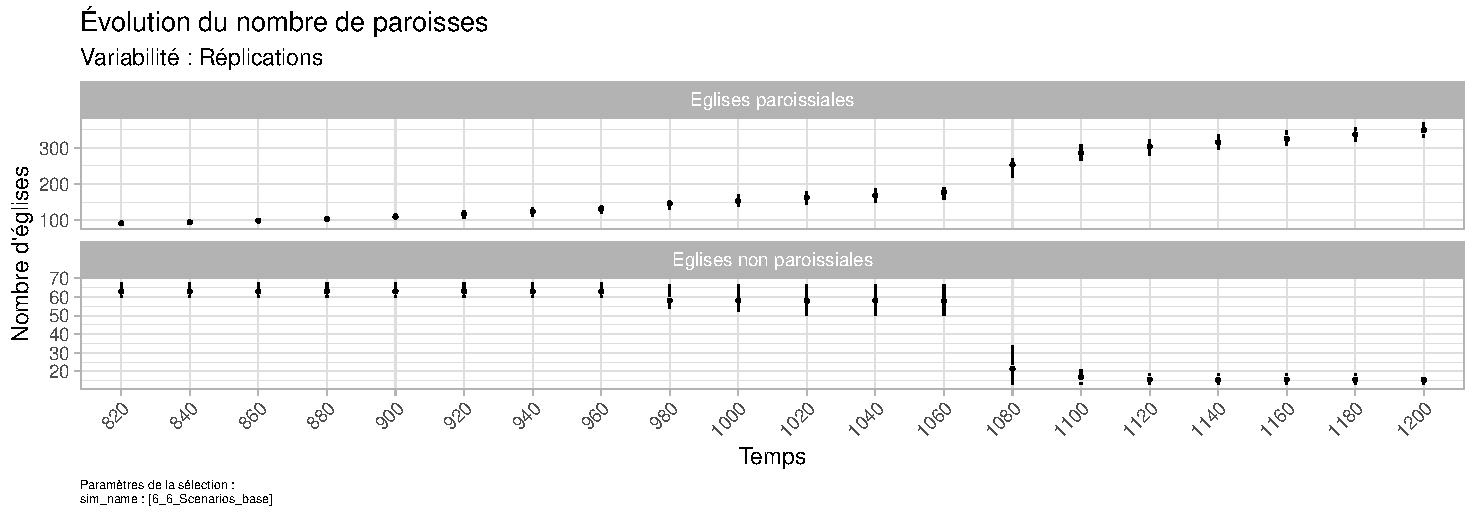
\includegraphics[width=\linewidth]{img/results_6_6/Paroisses_Nb_Haut.pdf}
	\caption{Nombre de paroisses.}
	\label{fig:results-paroisses-nb}
\end{figure}

On constate nettement dans la \cref{subfig:results-paroisses-carte} une densification généralisée du maillage paroissial.
Cette densification est visible à deux niveaux.
En premier lieu, le maillage est de plus en plus dense globalement : la superficie moyenne des paroisses diminue (visible aussi dans la \cref{subfig:results-paroisses-superficie}), et visuellement, on constate une certaine homogénéisation et normalisation des paroisses.
Les très grandes paroisses initiales (plus de 50 km² dans la \cref{subfig:results-paroisses-superficie}), surtout situées dans les marges de la région, disparaissent progressivement à mesure qu'elles sont subdivisées par le mécanisme de création/promotion d'églises paroissiales rurales (\hl{ref méca paroisse, chap2}).

\begin{figure}[H]
	\centering
	\hspace{5pt}
	\subfloat[Densité des paroisses et des paroissiens.\label{subfig:results-paroisses-carte}]{	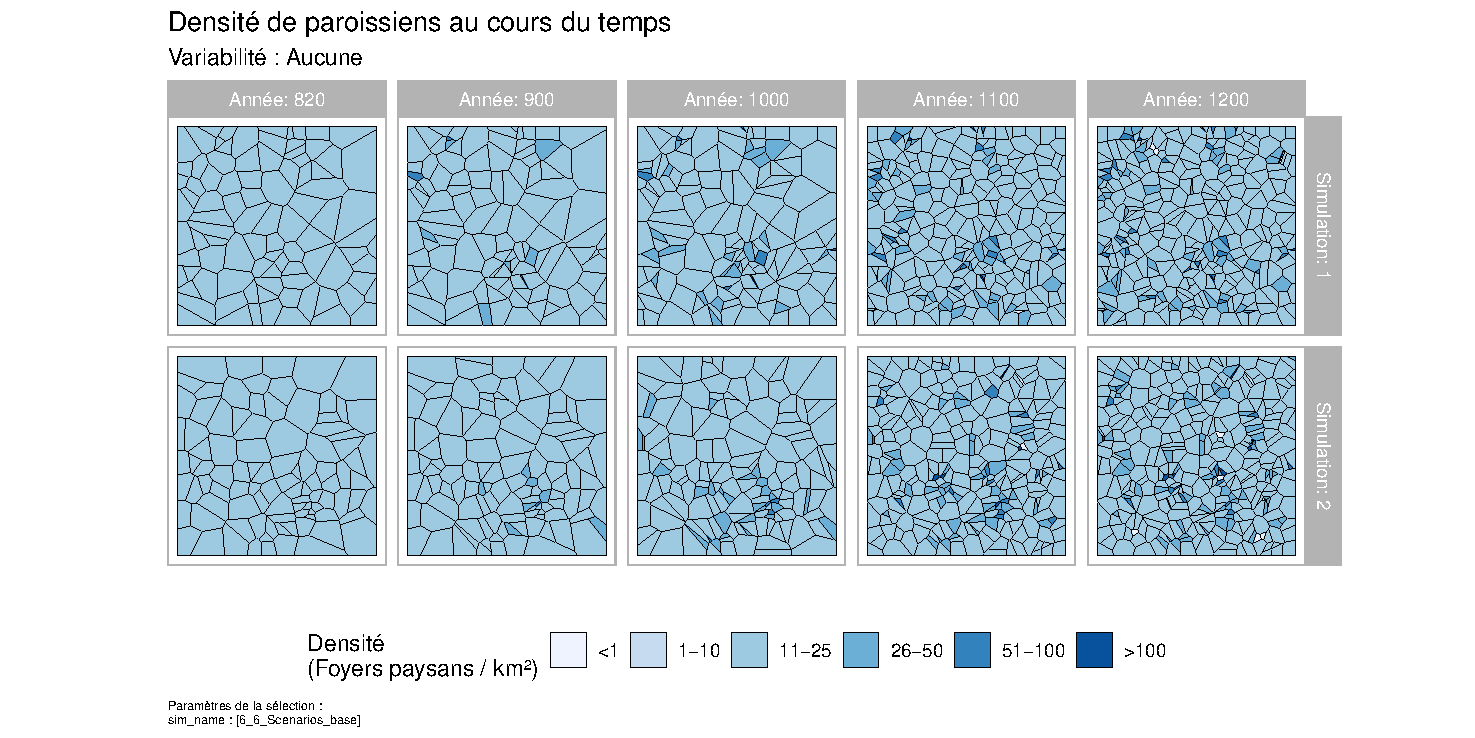
\includegraphics[width=\linewidth]{img/results_6_6/Paroisses_Carte_Haut.pdf}}
	\hspace{1em}
	\subfloat[Superficie des paroisses\label{subfig:results-paroisses-superficie}]{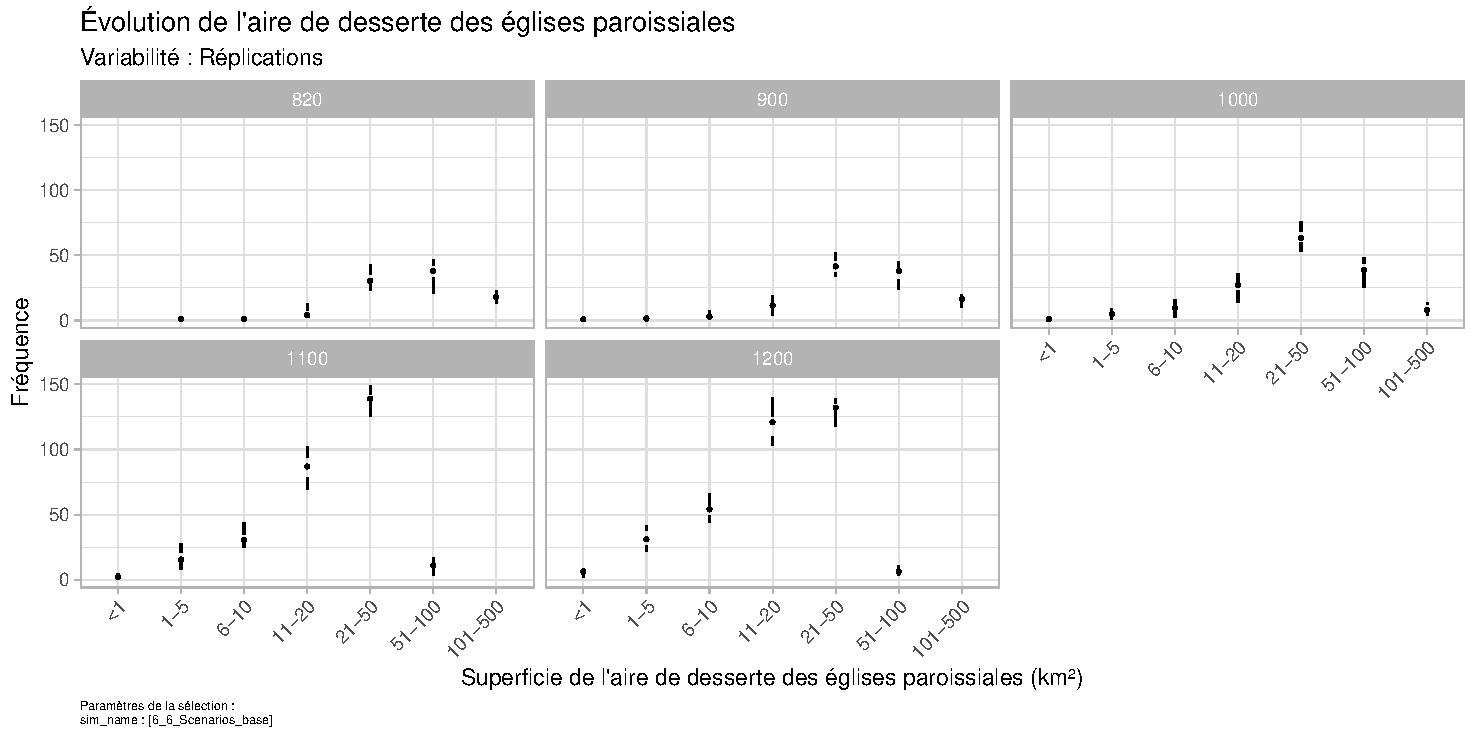
\includegraphics[width=\linewidth]{img/results_6_6/Paroisses_Superficie_Haut.pdf}}
	\caption{Indicateurs du maillage paroissial.}
	\label{fig:results-paroisses}
\end{figure}

En second lieu, à l'échelle infra-régionale, on note une intensification très locale de paroisses (le maillage augmente fortement), dans lesquelles les densités de foyers paysans sont importantes.
Ces densifications locales sont représentatives des agrégats les plus importants, qui peuvent comporter jusqu'à près d'une dizaine d'églises paroissiales\footnote{
	On peut le constater dans la \cref{fig:results-nb-poles-agregats}-a, où les pôles les plus importants de la hiérarchie contiennent une douzaine d'attracteurs. Si l'on considère que ces pôles contiennent un agrégat et un château, on peut en déduire qu'il y a aussi une dizaine d'églises paroissiales au service de cet agrégat.
}.

Ces deux niveaux d'observation, combinés à la cartographie des agrégats (\cref{fig:results-carte-agregats_poles}), montrent que le modèle produit bien une dispersion du peuplement dans l'espace : on voit des concentrations locales, mais à l'échelle globale, les mailles sont harmonisées par le bas, signe que des petits agrégats apparaissent dans l'ensemble du monde simulé.

\begin{figure}[H]
	\centering
	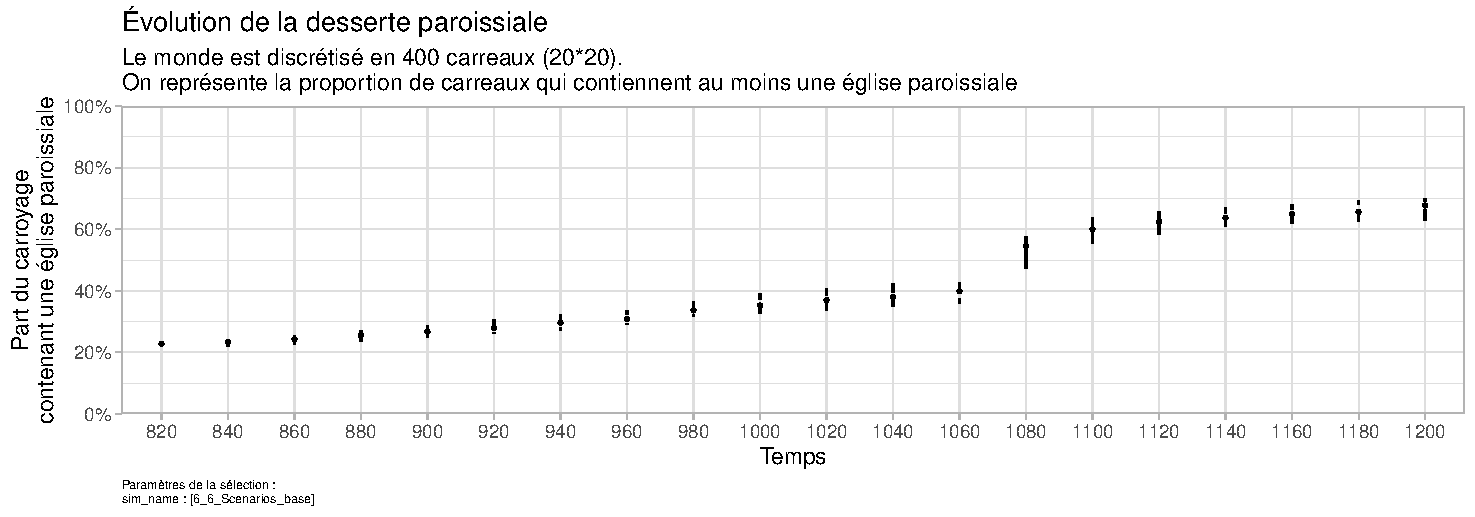
\includegraphics[width=\linewidth]{img/results_6_6/Paroisses_Desserte_Haut.pdf}
	\caption{Couverture de la desserte paroissiale.}
	\label{fig:results-paroisses-desserte}
\end{figure}

Pour préciser cette mesure et obtenir un indicateur spatial agrégé des réplications\footnote{
	Au contraire des cartes, qui ne peuvent décrire que des simulations particulières, l'agrégation spatiale n'étant pas possible dans le monde théorique fluctuant qui est simulé (voir \hl{chap7, agrégation} pour plus de précision).
}, on peut quantifier la couverture de l'espace qu'occupent les églises paroissiales.
Dans la \cref{fig:results-paroisses-desserte}, le monde simulé est discrétisé en 400 carreaux de 4 km de côté et on procède à un comptage de la proportion de ces carreaux qui contiennent au moins une église paroissiale à chaque date.
La lecture de la figure montre que la part du monde qui est située à proximité d'une église paroissiale augmente au cours du temps, avec un rythme comparable à celui de l'augmentation du nombre d'églises paroissiales (\cref{fig:results-paroisses-nb}).
Cela indique que l'augmentation du nombre de paroisses dans le modèle est bien un phénomène qui est réparti de manière homogène dans l'espace.
SimFeodal est donc bien en capacité de reproduire \textit{in silico} les processus de fixation et de dissémination qui ont été observés empiriquement en Touraine et plus généralement dans l'Europe du Nord-Ouest.



\bigskip

\paragraph[Conclusion intermédiaire]{}
SimFeodal parvient ici entièrement à reproduire le double fait stylisé recherché : fixation et dissémination du peuplement.
Pourtant, plus encore que pour les dimensions précédentes, il nous paraît extrêmement difficile d'aller plus loin dans le calibrage du modèle.
La raison en est principalement la difficulté de l'évaluation quantitative de ces phénomènes.
Parmi les indicateurs de sortie de simulation étudiés, ceux correspondant à cette dimension d'analyse sont les plus intrinsèquement spatio-temporels, et se prêtent donc mal à des agrégations synthétiques.
Certes, le champ de l'analyse spatiale s'est en partie constitué pour répondre à ce type de problème, en trouvant des mesures synthétiques et variées permettant de décrire et de comparer des semis de points, correspondent-ils à des entités ou à des époques différentes.

Pourtant, et on y reviendra plus extensivement dans le chapitre suivant, on constate ici une limite de notre méthode d'évaluation des simulations, au vu des données et connaissances empiriques dont on dispose.
Un espace théorique, simulé et très variable localement comme celui de SimFeodal se prête en effet mal à une agrégation de données.
Les différentes réplications d'un modèle ne partagent ainsi pas véritablement de référentiel spatial commun en dehors des limites du monde simulé : les positions des agrégats, des églises, des paroisses, sont en effet incomparables d'une réplication à l'autre.
Sans données empiriques susceptibles de préciser les taux d'occupation attendus, les mesures de dispersion des semis d'églises, de villages etc., on ne peut pousser l'évaluation visuelle plus avant.

%Pour pousser l'évaluation et être en mesure de comparer de nouvelles simulations par le biais des indicateurs présentés ici, au moins pour ceux relatifs à la fixation et dissémination, il faudrait sans doute mener des études de cas plus approfondies sur les sorties du modèle.
%On pourrait par exemple suivre des ensembles de foyers paysans ou d'agrégats tout au long des simulations pour analyser plus finement leur comportement.
%Mais même alors, le manque de sources empiriques se ferait forcément et fortement ressentir : on pourrait peut-être isoler la différence entre des simulations, mais serait-il vraiment possible de les départager ?

\subsection{Après le calibrage, comment affiner le modèle ?}

Dans l'ensemble, l'analyse des résultats montre que cette version calibrée de SimFeodal répond aux attentes en matière de reproduction des faits stylisés identifiés d'après les connaissances expertes.
Le modèle aboutit bien sur une polarisation de l'habitat, autour de pôles d'attractions très hiérarchisés et disséminés dans l'espace simulé.
Cette polarisation débouche sur une structure spatiale pérenne, due à la fixation des foyers paysans au sein d'agrégats qui composent le système de peuplement.

Le modèle SimFeodal est donc satisfaisant vis-à-vis de ce pour quoi il a été conçu, développé et calibré.
En comparant les dizaines de versions successives du modèle, ce constat est d'autant renforcé : chaque version a permis des améliorations notables, depuis une version 0 qui parvenait tout juste à une concentration du peuplement jusqu'aux versions plus récentes, préalables à la version 6.6 ici présentée, qui ont renforcé l'ajustement aux connaissances expertes chacune sur des points plus spécifiques.
Certains indicateurs, toutefois, et en particulier les indicateurs quantitatifs qui donnent un aperçu global et synthétique des résultats du modèle (\cref{ssec:results-global}), demeurent toutefois relativement éloignés des objectifs fixés.
On pourrait donc chercher désormais à prolonger et affiner le calibrage du modèle afin que sa capacité à reproduire les faits stylisés soit améliorée.

Il nous semble toutefois que cette démarche ne vaudrait pas le temps et l'effort qu'il serait nécessaire de lui consacrer.
Nous appuyons ce sentiment sur deux raisons principales, la première liée au domaine de l'empirie et la seconde au domaine du modèle.

\paragraph{Calibrer sans sur-ajuster.}
Dès le calibrage des paramètres d'\textit{input} (\cref{sssec:calibrage-inputs}), on mentionnait les difficultés du recueil de sources empiriques -- matérielles ou littéraires -- pour des éléments qui paraîtraient pourtant triviaux et indispensables à tout géographe contemporain.
La population de la région et son évolution sur la période considérée, par exemple, ne peut donner lieu qu'à une estimation très grossière.
De plus, on ne peut avoir aucune garantie, ni même d'espoir, que de futures sources permettent de mieux les spécifier.

Dans le même temps, on cherche à améliorer l'ajustement des sorties du modèle à des objectifs fixés sur ces sources empiriques floues et lacunaires.
L'expertise des thématiciens du groupe de modélisation de SimFeodal a permis de définir ces objectifs, mais ceux-ci présentent un niveau de précision parfois assez faible.
Par exemple, on cherche à ce que SimFeodal puisse atteindre 20\% de foyers paysans isolés en fin de simulation.
Les versions successives du modèle ont permis de faire descendre ce taux d'environ 60\% à environ 20\%.
En considérant que les connaissances empiriques donnent une estimation plausible située entre 20\% et 30\%, quel sens y aurait-il à départager des modèles selon qu'ils atteignent 25\% ou 27\% ?

Ce problème, qui se pose pour chacun des objectifs et attendus du modèle, est un cas typique de sur-ajustement, ou \og overfitting\fg{}.
Sur le plan thématique, chercher à coller absolument à un objectif sans tenir compte du degré d'incertitude de ce dernier, bien plus élevé que celui que le modèle est en mesure de produire, n'a ainsi aucun sens.
Sur le plan méthodologique, on peut aussi noter qu'à mesure que le calibrage du modèle progresse, les \og gains\fg{} de chaque étape se font plus faibles.
Chercher à améliorer le calibrage du modèle reviendrait alors à différencier des modèles sur des critères de plus en plus précis, alors même que le niveau de précision de ces critères est en lui-même statique et d'un ordre de grandeur inférieur.

Sans connaissances empiriques supplémentaires, il n'est pas possible de véritablement mieux calibrer SimFeodal, qui a déjà atteint un niveau de détail qui dépasse presque celui des connaissances expertes par le prisme desquelles tout résultat doit être étudié pour porter un sens.


\paragraph{Calibrer un modèle (très) complexe.}
Un autre élément concoure aussi à la difficulté d'améliorer le modèle, cette fois-ci directement lié aux choix de conception de SimFeodal.
Comme décrit dans les deux premiers chapitres, SimFeodal est un modèle exploratoire, plus descriptif (KIDS) que parcimonieux.
Les paramètres y sont très nombreux, de même que les mécanismes qu'ils ajustent.
Les agents du modèle interagissent, et, avec eux, les mécanismes qui les caractérisent sont aussi entrecroisés et imbriqués.
Si l'on a une connaissance parfaite de chaque mécanisme (puisqu'on les a conçus et implémentés), il est difficile d'avoir une connaissance de même ordre sur l'aboutissement de leurs interactions, c'est la raison d'être de la simulation.

Dans des modèles moins descriptifs, mêmes complexes, on peut avoir des idées relativement précises de la combinaison des mécanismes, et donc une bonne intuition des sorties de simulation qui en aboutiront.
Dans un modèle comme SimFeodal, les paramètres sont trop nombreux pour que ce soit réellement possible, et les résultats contre-intuitifs ont été fréquents dans les différentes étapes de paramétrage et de calibrage du modèle.
Ces éléments contre-intuitifs, surprenants, sont extrêmement stimulants du point de vue de la connaissance des effets du modèles.
Ils placent les modélisateurs et évaluateurs dans une démarche abductive où l'identification de l'explication de ces contre-intuitions permet de mieux comprendre le fonctionnement effectif du modèle et à partir de là du système modélisé.

Dans la recherche d'un calibrage mieux adapté, cette approche abductive ne permet toutefois pas véritablement de progresser.
À mesure que le calibrage se précise, la complexité du modèle apparaît renforcée.
Comme dans le principe des vases communicants, une modification de valeur d'un paramètre est presque systématiquement assortie d'une réaction imprévu (et imprévisible) sur un indicateur différent de celui sur lequel le paramètre devait agir.
Chaque modification de paramètre devrait donc donner lieu à de nouveaux ajustements d'autres paramètres, jusqu'à obtenir un ensemble de valeurs de paramètres stable.

Pour améliorer le calibrage, et éviter ces allers-retours imprévisibles entre paramètres, il manque alors une vision plus globale des réactions engendrées par les modifications de chaque paramètre
Une telle vision permettrait de ré-organiser les paramètres, pour chaque indicateur de sortie, en ensembles thématiques dont l'on ferait systématiquement co-varier les valeurs testées afin d'approcher de l'objectif de manière harmonisée.
Pour mieux comprendre les aboutissements du modèle, il est dès lors nécessaire de l'explorer de manière plus systématique, en essayant de comprendre l'influence réelle de chacun des paramètres plutôt que de tâtonner, de manière experte certes, en agissant sur les paramètres qui nous semblent intuitivement les plus importants.
%Une telle exploration, plus systématique, de grande ampleur et cherchant à dépasser l'intuition, ne peut se mener que sur une quantité réduite d'éléments du modèle (indicateurs de sortie, mais aussi intervalle de validité des paramètres), et cela requiert dès lors de réussir à synthétiser de manière manifeste, quantifiée, les attentes que l'on a vis-à-vis des résultats du modèle.
Ce sont ces objectifs de compréhension plus fine du comportement du modèle que nous allons poursuivre dans la suite de ce chapitre, au moyen d'analyses de sensibilité.


\clearpage
\section{Analyser la sensibilité de SimFeodal \label{sec:ana-sensib}}

Parmi les nombreuses méthodes dédiées à l'évaluation de modèles, il en est une que l'on retrouve dans tous les manuels et dans la plupart des articles dédiés à la présentation de modèles.
Il s'agit de l'analyse de sensibilité, catégorie en fait plurielle qui regroupent l'ensemble des méthodes voués à tester ou à explorer la stabilité d'un modèle face aux éléments qui le composent : poids des \textit{inputs} dans les résultats obtenus, variabilité des résultats selon les valeurs de paramètres choisies, variabilité des résultats due à l'aléa etc.
Ces méthodes sont extrêmement nombreuses et constituent presque un champ scientifique entier, lié à l'évaluation de modèles, soient-ils à base d'agents ou statistiques.

Parmi celles-ci, les méthodes les plus classiques \autocite[257]{crooks_agent-based_2019} visent à \og déterminer l'influence des paramètres sur les sorties du modèle.\fg{} \autocite[75]{ginot2005explorer}.
Il s'agit de faire varier les valeurs des paramètres et de mesurer les écarts résultant dans les sorties.
Le plus souvent, cette mesure est quantitative, par exemple sous la forme d'un \og indice de sensibilité\fg{} qui dépend des variations des sorties mais aussi de l'amplitude de la variation des paramètres\footnote{
	Cette prise en compte de la variation des valeurs de paramètre, par exemple dans l'indice proposé par \textcite[258]{crooks_agent-based_2019} et dérivé de celui de \textcite{hamby_review_1994} (in \cite[201]{osullivan_spatial_2013}), permet de s'assurer, lors de la comparaison de la sensibilité des paramètres, que les valeurs comparées sont bien comparables.
	Pour prendre l'exemple du modèle de Schelling, il s'agit de s'assurer qu'on ne compare par une variation de 0,1\% du seuil de tolérance avec une variation de 20\% dans la part d'espace vide.
}.

Les analyses peuvent être menés en croisant des valeurs pour tous les paramètres, c'est-à-dire en analysant la sensibilité du modèle aux interactions entre paramètres.
On peut aussi procéder paramètre par paramètre, en conservant par exemple des valeurs fixes pour un jeu de paramètre (issus de calibrage) de base et en faisant varier un unique paramètre à la fois (analyse de type \textit{OFAT}, \og \textit{one factor at a time}\fg{}).

Les analyses de sensibilités sont largement recommandées comme une pratique indispensable à la validation de modèle, mais nous avons décrit dans le \hl{chapitre 3} la démarche que nous avons préféré pour l'évaluation de SimFeodal.
L'analyse de sensibilité est toutefois un outil extrêmement utile pour aider à la compréhension d'un modèle, sans chercher à en quantifier la validité.
Cette méthode repose sur l'exploration d'un modèle par le prisme de ses réactions face aux paramètres choisis, et permet ainsi de mener une étude approfondie de l'influence des paramètres.
Dans certains modèles, une analyse de ce type a par exemple permis de rendre plus parcimonieux un modèle KISS, en mettant en lumière le peu d'influence d'un paramètre sur l'ensemble des sorties d'un modèle.
C'est le cas dans le travail de thèse de \citeauteur{schmitt_modelisation_2014}, où une analyse de sensibilité a révélé la relative inutilité de l'un des 6 paramètres mobilisés dans le modèle SimpopLocal \autocite[224-225]{schmitt_modelisation_2014}.
Dans le cadre d'un modèle exploratoire, où les très nombreux paramètres comportent vraisemblablement une part de redondance, l'ambition n'est pas de réduire la masse de paramètres, mais plutôt d'aider à comprendre lesquels ont la plus grande influence sur le modèle.

Dans le cadre de SimFeodal, une analyse de sensibilité doit permettre, comme l'évaluation visuelle, de gagner en compréhension sur le modèle, et en conséquence sur les dynamiques modélisées.

La nature exploratoire et descriptive de SimFeodal rend l'application des méthodes classiques de l'analyse de sensibilité assez difficile : les paramètres ne sont pas tous quantitatifs, certains fonctionnent par paires, par grappes etc.
De manière plus générale, une analyse de sensibilité quantitative requiert à minima des objectifs quantitatifs synthétiques, hiérarchisés et parcimonieux, ce qui n'est pas la démarche empruntée dans SimFeodal.

Dans cette partie, nous nous en tiendrons à une analyse de sensibilité grossière, orientée vers une évaluation visuelle, à l'instar des autres démarches d'évaluation du modèle mises en places.
Nous nous inscrivons pleinement dans le raisonnement de \citeauteur{hirtzel2015exploration}, d'autant plus que le dit raisonnement est tenu dans une thèse dont l'analyse de sensibilité de modèles descriptifs est l'un des enjeux principaux :
\begin{quotation}
	\og Ces différents constats nous ont conduit à procéder à des analyses de sensibilité locales, avec la méthode OAT\footnote{
		[C'est un autre acronyme de \og \textit{one factor at a time}\fg{}, identique à \textit{OFAT} que nous utilisons dans cette partie.]
	}, en modifiant les valeurs de chacun des paramètres les unes après les autres, toutes choses égales par ailleurs, c’est-à-dire tous les autres paramètres étant fixés à leur valeur par défaut \textelp{}.
	Ce choix n’est pas unique dans la modélisation individu-centrée : la méthode OAT est utilisée dans plusieurs travaux en géographie ou en écologie (Ginot et al., 2006; Sanders et al., 2006; Laperrière et al., 2009; Schouten et al., 2014).
	
	Nous n’avons pas jugé indispensable le calcul d’indices de sensibilité pour étudier la sensibilité des résultats de simulation aux différents paramètres du modèle.
	Une analyse graphique à la manière de Sanders et al. (2006\st{a}), Laperrière et al. (2009) ou encore Schouten et al. (2014) nous a paru suffisante, dans un premier temps.
	Ainsi, pour reprendre les termes évoqués dans les deux sous-parties précédentes, l’analyse de sensibilité présentée dans ce chapitre est une analyse locale (OAT), avec des évaluations qualitatives de l’impact de l’incertitude émanant des valeurs de paramètres sur différents résultats de simulation.\fg{}\\
	\mbox{}~ \hfill \cite[251-252]{hirtzel2015exploration}
\end{quotation}


\subsection{Méthodologie - Analyse visuelle de sensibilité}

Dans cette partie, nous décrivons et justifions brièvement la méthodologie mise en place pour l'analyse de sensibilité de SimFeodal.
Les sources informatiques, précises, de la démarche sont disponibles dans le dépôt du modèle (\hl{mettre URL dossier}).
Le détail des paramètres, les outputs du modèle, les traitements et les sorties graphiques sont disponibles quand à eux à cette adresse : \hl{depot these / anasensib}

\subsubsection{Calcul de la sensibilité}

Nous avons choisi de mener l'analyse de sensibilité de SimFeodal en empruntant l'approche \textit{OFAT}, c'est-à-dire en faisant varier les paramètres un par un.
Dans un modèle complexe où les agents sont en interactions les uns avec les autres, cette approche est forcément biaisée et lacunaire au regard d'approches plus avancées comme les méthodes d'exploration de l'espace des paramètres.
Pourtant, c'est la seule qui nous semblait applicable dans le cas de SimFeodal.
Il convient en effet de rappeler que ce modèle est caractérisé par un nombre important de paramètres : près de 70.
En ne choisissant que 5 valeurs pour chaque paramètre et pour croiser tous les paramètres, une analyse de type plan complet demanderait alors l'exécution de $5^{70} \times 20_{\text{[replications]}}$, soit environ $10^{50}$ simulations\ldots

\paragraph{Paramètres}

Dans une analyse de sensibilité, le premier choix à faire concerne les paramètres à analyser.
Dans les modèles statistiques ou KISS, l'analyse de chacun des paramètres est une évidence.
Dans des modèles plus descriptifs tels que SimFeodal (ou les modèles analysés par \textcite{hirtzel2015exploration}), on procède souvent à une sélection des paramètres afin de réduire l'ampleur de la tâche.
Par exemple, quand certains paramètres ont un ancrage empirique fort, on peut considérer qu'ils se comportent plus comme des constantes que comme des paramètres, n'auront jamais à varier, et ne requièrent ainsi pas d'être analysés.

Dans SimFeodal, on aurait pu par exemple se passer d'analyser les paramètres de contexte les plus inscrits dans les connaissances empiriques.
Pourtant, comme nous envisageons d'éprouver le modèle sur des scénarios hétérogènes, par exemple portant sur des régions et des périodes différentes, il nous a semblé important de tester aussi ces paramètres.
On a opté pour une analyse de sensibilité de chacun des paramètres du modèle.
SimFeodal comporte dans les faits 70 paramètres, mais en pratique, le nombre de paramètres sur lesquels on peu réaliser des analyse est plus faible.
Ainsi, certains paramètres n'ont aucun sens quand mobilisés seuls.
Par exemple, deux paramètres définissent le rayon minimum et maximum des zones de prélèvement.
Il n'y a pas grand sens à faire varier l'un sans l'autre.
Dans l'analyse de sensibilité, nous considérons ces deux paramètres comme un unique paramètre à analyser, qui ne prend pas la forme d'une valeur numérique simple, mais plutôt celle d'une étendue.

Pour cette analyse de sensibilité, nous avons au final analysé 57 \og paramètres\fg{}, certains de forme numérique simple, d'autres sous formes d'étendues, et enfin quelques-uns ayant des structures plus complexes (étendues changeant au cours du temps par exemple).

\paragraph{Méthode}

La méthode choisie est simple : on définit un jeu de paramètres de base, issu du calibrage, et pour chacun des paramètres, on exécute un ensemble de simulations en faisant varier ce paramètre autour de sa valeur de base.
Comme pour toute simulation d'un modèle stochastique, il est indispensable de procéder à des réplications de ces simulations.

Comme le nombre de paramètres était déjà important, que le nombre de réplications (20) l'était lui aussi, on a choisi de mener une analyse de sensibilité assez réduite, en ne testant, pour chaque paramètre, que 5 valeurs différentes.
Ce nombre est assez faible, mais amène déjà à l'exécution de $57_{\text{[paramètres]}} \times 5_{\text{[valeurs]}} \times 20_{\text{[réplications]}} = 5700$ simulations, ce qui est une quantité importante de simulations au regard de toutes celles qui ont été mené dans les étapes de paramétrage et d'évaluation visuelle du modèle.

\paragraph{Étendue}
\label{par:etendue-parametres}

Dans une analyse de sensibilité classique, on cherche à mener des variations de paramètres comparables, c'est-à-dire centrées autour des valeurs par défaut et présentant des variations relatives de de même ampleur.
Par exemple, pour un modèle dont le premier paramètre vaut 10 et le second 100, on cherchera à répartir les valeurs testées de manière comparable : 
le premier paramètre sera testé aux valeurs 0, 5, 10, 15 et 20, et le second pour 0, 50, 100, 150 et 200.

Dans un cas réel, cette règle est difficile à suivre : on a ici pris l'exemple de paramètres quantitatifs \og de stock\fg{}, qui ne sont comparables qu'entre eux.
Dans SimFeodal, certains paramètres ont des structures bien plus difficilement comparables, à l'instar des étendues plus haut.
Comment rendre comparable cinq variations autour de 10 et cinq variations autour de l'étendue [1500m; 5000m]?
L'étendue des possibles transformations pour ces étendues est bien plus important : diminution, augmentation, translation\ldots

Ce problème se pose de manière plus importante encore pour les paramètres qui évoluent en fonction du temps.
Par exemple, le paramètre , qui agit sur la satisfaction protection des foyers paysans, a une valeur composite (de type \textit{map}, voir \cref{lst:maps-gama} dans le \hl{chapitre 2}) qui vaut \og $0$ entre 800 et 940; $0.2$ en 960 ; $0.4$ en 980 ; $0.6$ en 1000 ; $0.8$ en 1020 ; et $1$ à partir de 1040\fg{}.
Pour l'analyser dans son entièreté, il faudrait supprimer la variation en testant plusieurs valeurs, mais aussi changer le rythme de cette variation, en décaler l'étendue temporelle, en changer l'intensité etc.
Sous bien des aspects, ce paramètre peut être considéré comme qualitatif, et les variations qu'on lui appliquera dans l'analyse de sensibilité ne peuvent être que très subjectives et intrinsèquement différentes.

Face à ces difficultés, nous avons adopté une position générale acceptant la subjectivité, la non comparabilité, mais cherchant à explorer des valeurs \og caractéristiques\fg{} pour ce type de paramètres : activation et désactivation du mécanisme associé, valeur de base, et augmentation et diminution de l'ampleur de la valeur de paramètre.
Dans l'ensemble, les valeurs de paramètres choisies (\hl{mettre les tableaux en annexe}) ne sont que peu comparables de manière numérique, mais cela n'empêche en rien qu'elles apportent un éclairage précieux sur le comportement du modèle en fonction de ses paramètres.

\paragraph{\textit{Outputs}}

Le \hl{chapitre 5} donnait des ordres de grandeur correspondant à la masse de données produites par le modèle pour une simulation, autour de 10 Mo.
Avec 5700 simulations, un enregistrement complet des données aurait représenté plus de 50 Go de données et plus de 50 milliards de lignes de données à pré-traiter, intégrer et analyser dans la base de données.
Pour une analyse qui n'est pas au cœur de notre démarche de co-construction, cela représentait un poids bien trop important.
Nous avons choisi de réduire autant que possible la production d'indicateurs de sorties de simulations pour cette analyse de sensibilité.

Dans un premier temps, nous n'enregistrons l'état du modèle qu'à son pas de temps final (en 1200) plutôt que tout au long de son déroulement.
On perd certes l'aspect dynamique et la possibilité de comparer les rythmes entre les simulations, mais comme l'analyse de sensibilité doit se concentrer sur aussi peu d'objectifs que possible, ce n'est pas véritablement gênant.
Pour les mêmes raisons, on a aussi décidé de n'extraire que des données très agrégées du modèle : l'analyse de sensibilité s'appuie sur des résultats à l'échelle globale du modèle, et il n'est à ce moment nul besoin d'enregistrer les indicateurs individuels des agents du modèle.

La sélection des indicateurs agrégées a été assez rapide : on a choisit de reprendre les indicateurs numériques synthétiques, qui reprennent le tableau des objectifs présenté en \cref{tab:objectifs-types}.
Parmi ceux-ci, on a conservé uniquement les 6 indicateurs \og émergents\fg{} : 
nombre d'agrégats; nombre de grands châteaux; nombre d'églises paroissiales; distance moyenne entre églises paroissiales; part de foyers paysans isolés; augmentation de la charge fiscale
	
Dans la construction et l'évaluation du modèle, ce sont ces indicateurs que l'on a le plus observés, et s'ils n'informent pas sur l'ensemble des objectifs thématiques du modèle, ils permettent au moins de qualifier sommairement son comportement d'ensemble.

\paragraph{Computation}

Dans une analyse de sensibilité portant sur autant de simulations, la masse de données n'est pas la seule limite.
Le temps de calcul l'est tout autant, sinon plus, tant il peut s'étendre rapidement.
Sur un ordinateur individuel, avec les valeurs de paramètre décidées après calibrage, chaque simulation demande en moyenne 5 minutes de calcul.
Multiplié par les 5700 simulations requises, l'exécution des simulations nécessaires à l'analyse de sensibilité réclame alors un temps de calcul de près de 20 jours sur un ordinateur individuel, sans véritable droit à l'erreur sous faute de recommencer ce quasi-mois de calcul.

Pour que cette analyse soit effectuée dans un délai plus raisonnable, nous avons utilisé les capacités de calcul d'un serveur du laboratoire ainsi que d'un serveur de calcul géré par la TGIR Huma-Num.
En distribuant les exécutions de simulation sur la quarantaine de processeurs informatiques que cela représentait au total, tout en laissant tourner les simulations uniquement de nuit pour ne pas gêner les autres utilisateurs de ces serveurs, toutes les simulations requises ont été exécutées en 3 jours, ce qui représente cette fois-ci un investissement temporel bien plus raisonnable.

\subsubsection{Analyse Quantitative - Filtrage des paramètres}

Devant la masse de paramètres à analyser, nous avons réalisé qu'il était difficile de mener une analyse visuelle directe de la sensibilité des paramètres.
Il a été choisi de mener une première étape, quantitative, pour permettre de trier et de filtrer un sous-ensemble de paramètres dont une étude plus approfondie serait alors possible.

Pour cette étape, on a raisonné à l'échelle agrégée du paramètre, en cherchant à mesurer la variabilité des indicateurs de sortie choisis provoquée par la variation des valeurs de paramètres.

\paragraph{Normalisation des objectifs}

Un premier problème est que les indicateurs de sortie de simulation choisis, les objectifs, sont très hétérogènes en termes d'ordre de grandeur.
Il était alors nécessaire de procéder à un \og centrage\fg{} des données issues de la simulation.
Ce centrage peut être effectué, classiquement, sur les valeurs obtenues, pour obtenir une moyenne valant 0, comme on le fait lors d'une normalisation classique de données.

Pour l'étude de SimFeodal, nous avons préféré centrer les données de chaque indicateur relativement aux objectifs numériques identifiés.
Par exemple, une simulation produisant 250 agrégats, quand l'objectif numérique est de 200, aura pour indicateur \og nombre d'agrégats\fg{} 50.
Cela permet de mesurer les comportements de manière plus thématique qu'un centrage statistique autour de 0.
Pour chaque indicateur, on a soustrait à la valeur obtenue par simulation la \og valeur attendue\fg{}, identifiée thématiquement comme objectif (voir le \cref{tab:results-basique}).
Après cela, pour chaque indicateur pris individuellement, les données générées par chaque simulation deviennent comparables.

Pour atteindre une comparabilité plus importante entre des données hétérogènes, on procède aussi usuellement à une \og réduction\fg{} des données, c'est-à-dire à la normalisation de leur variabilité (écart-type).
Classiquement, cette étape consiste à diviser chaque résultat par l'écart-type.
On obtient ainsi, pour chaque série de donnée, un écart-type de 1, qui permet alors de comparer la variabilité de ces séries hétérogènes.
Comme pour le centrage, on a choisi de réduire les données en fonction de données connues plutôt qu'autour d'une valeur abstraire de 1.
On a préféré pour cela se référer à nos données simulées de référence, c'est-à-dire issues des simulations présentées dans la première partie de ce chapitre, après calibrage.
Les données centrées ont ainsi été ensuite divisées par l'écart-type mesuré sur les simulations de cette version de référence, pour chaque indicateur numérique.

Au final, ce procédé de normalisation est très proche d'une normalisation statistique classique, mais se base sur des valeurs qui ont un sens dans le modèle plutôt que sur les valeurs \og abstraites\fg{} que constituent une moyenne à 0 et un écart-type de 1.

\vspace{-2em}\begin{flalign*}
& \text{valeur\_normalis\'ee}_{\text{indicateur\_i}} = & 
\frac{
 	\text{valeur}_{\text{indicateur\_i}} - \text{valeur\_attendue}_{\text{indicateur\_i}}
 }{
 \sigma(\text{valeurs\_calibr\'ees}_\text{{indicateur\_i}})
} &
\end{flalign*}

Ainsi conçue, la valeur normalisée permet une comparabilité au sein des indicateurs, mais aussi entre eux puisque les ordres de grandeur sont désormais similaires.

\paragraph{Calcul de la sensibilité}

Comme les valeurs sont désormais normalisées, il est possible de mener des opération conjointes sur les différents indicateurs.
On définit un indice global, intitulé \og sensibilité\fg{}, qui correspond à une moyenne, pour chaque paramètre, de ses valeurs normalisées dans chacun des indicateurs.
Après le centrage, les valeurs deviennent négatives ou positives selon qu'elles sont inférieures ou supérieures aux objectifs.
Pour un paramètre qui verrait des variations importantes, négatives et positives, le risque d'une moyenne est alors que la sensibilité calculée soit faible, le très positif compensant le très négatif.
Pour prévenir ce risque, on a choisi de calculer la sensibilité sur les valeurs absolues des valeurs normalisées plutôt que sur leur valeur brut.
La sensibilité de chaque paramètre peut alors être définie comme suit :

\vspace{-2em}\begin{flalign*}
& \text{sensibilit\'e}_{\text{param\`etre}\_\upalpha} = \\
& \frac{1}{n_{\text{indicateurs}}
	\times n_{\text{valeurs\_param\`etres}\_\upalpha}
	\times n_{\text{r\'eplications}}}
\sum |\text{valeurs\_normalis\'ees}_{\text{param\`etre}\_\upalpha}|
\end{flalign*}

\paragraph{Sélection de paramètres}

En calculant la sensibilité de chaque paramètre, on sera en mesure d'en sélectionner un sous-ensemble afin de procéder à une analyse visuelle de la sensibilité de ces derniers.
Pour isoler ce sous-ensemble, on ne conservera que les paramètres à la plus forte sensibilité globale, en cherchant à en conserver une dizaine.
Ce nombre est volontairement imprécis puisqu'il dépendra surtout de la forme de la distribution de la sensibilité des paramètres : on cherchera avant tout à isoler des paramètres dont la sensibilité les différencie franchement des autres.
On se basera pour cela sur une méthode entièrement subjective d'examen visuel des écarts entre les valeurs de sensibilité, tel qu'on peut le faire pour choisir un nombre de classes à étudier lors de l'exécution d'une classification ascendante hiérarchique.

Un risque de cette méthode est que certains indicateurs peuvent contribuer bien davantage que d'autres à la sensibilité d'ensemble, malgré la normalisation.
Pour ne pas risquer de négliger des paramètres dont la sensibilité s'exprimerait uniquement sur certains indicateurs, on complètera la sélection de paramètres précédente par une sélection des trois paramètres les plus sensibles sur chacun des 6 indicateurs.

\vspace{-2em}\begin{flalign*}
& \text{sensibilit\'e}_{\text{param\`etre}\_\upalpha_{\text{indicateur\_i}}} = \\
& \frac{1}{n_{\text{valeurs\_param\`etres}\_\upalpha}
	\times n_{\text{r\'eplications}}}
\sum |\text{valeurs\_normalis\'ees}_{\text{param\`etre}\_\upalpha_{\text{indicateur\_i}}}|
\end{flalign*}


En considérant qu'une large partie de ces paramètres auront vraisemblablement déjà été isolés par le filtre sur la sensibilité globale, on devrait obtenir quelques paramètres supplémentaires sur lesquels mener l'analyse visuelle.

\subsubsection{Analyse visuelle}

Une fois les paramètres à étudier sélectionnés, on pourra alors mener une analyse visuelle pour comprendre l'influence des paramètres sur les indicateurs de sortie du modèle.
Le nombre de paramètres étant réduit, il sera possible d'analyser l'importance de cette influence (la sensibilité), mais aussi sa cardinalité : en observant la réaction des indicateurs de sortie en fonction des valeurs de paramètre, on
pourra noter les corrélations (visuelles).

Cette analyse visuelle de sensibilité s'inscrit ainsi dans une analyse à la fois technique et thématique de SimFeodal.
Elle doit en effet permettre de gagner en compréhension sur les interactions entre paramètres et mécanismes.
Cela devrait éclairer l'aspect technique, lié à la validation interne du modèle -- tel paramètre que l'on pense jouer sur tel mécanisme se comporte-t-il bien comme attendu ? -- et l'aspect thématique -- est-ce que la taille du monde simulé a 


\paragraph{Visualisation}

L'objectif de la visualisation de la variation des paramètres est d'observer, pour chaque paramètre, comment ce dernier varie sur chacun des indicateurs.
Pour cela, on représente la variation due aux réplications de chaque paramètre au moyen de représentations visuelles dédiées à la variabilité, comme des \textit{box-plots} ou \textit{violin-plots}.
La \cref{fig:exemple-visu-sensib} présente un exemple de mise en page de telles représentations graphiques afin de faciliter l'analyse de sensibilité visuelle.
\begin{figure}[H]
	\centering
	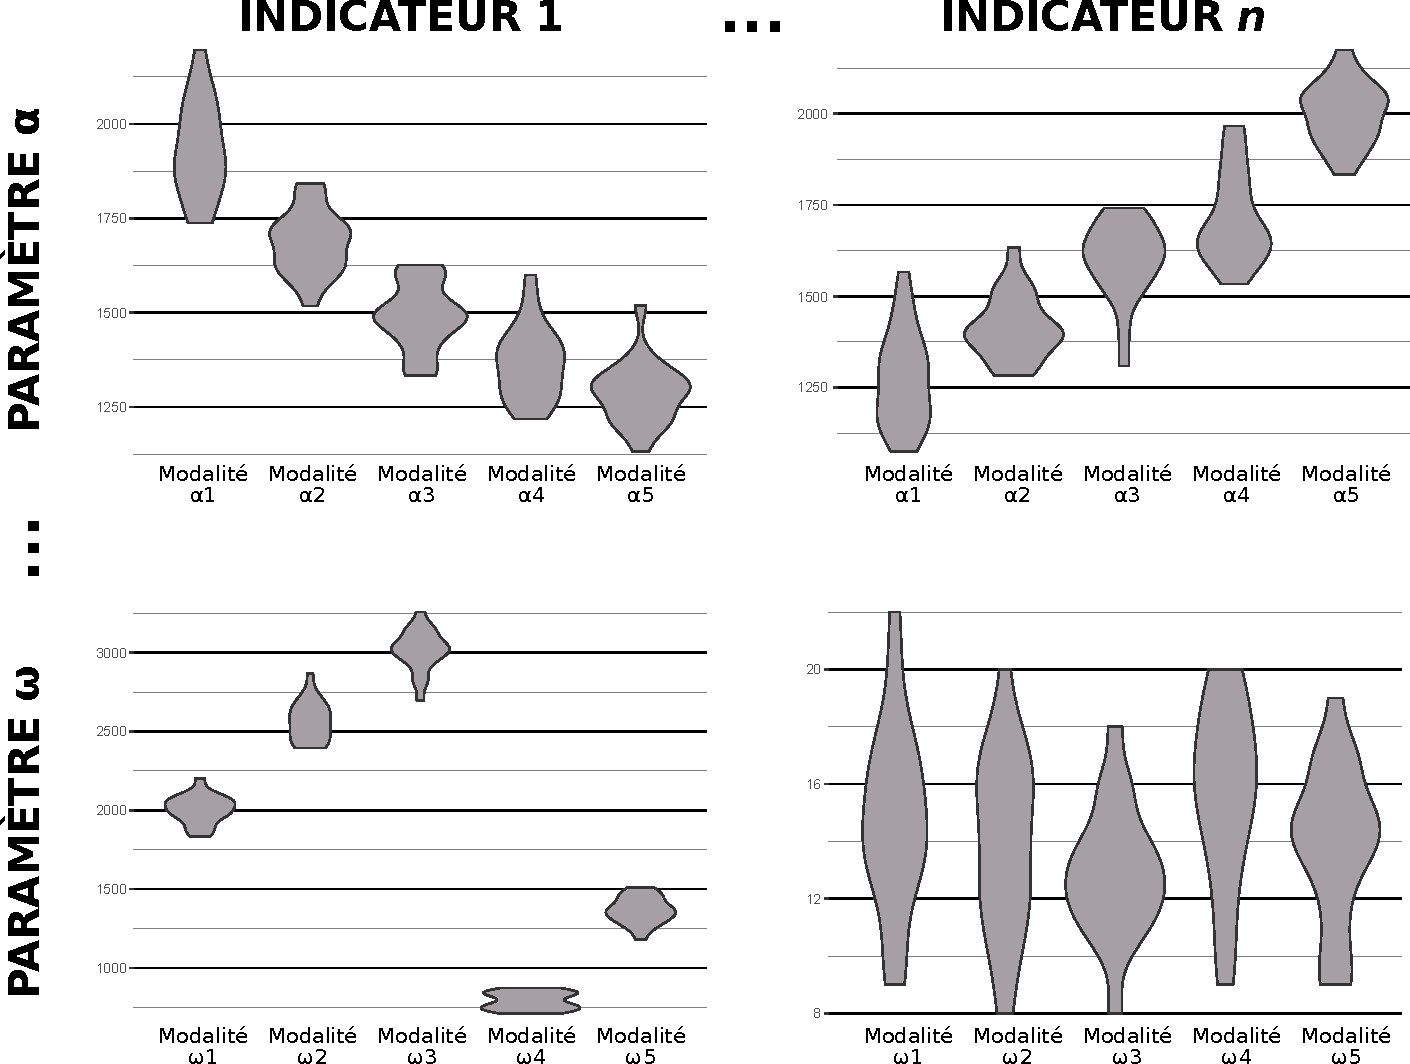
\includegraphics[width=.9\linewidth]{img/schema_violinplots_sensib.pdf}
	\caption{Construction et mise en page de planches graphiques dédiés à l'analyse visuelle de la sensibilité des 5 modalités de $\upomega$ paramètres sur \textit{n} indicateurs.}
	\label{fig:exemple-visu-sensib}
\end{figure}

\paragraph{Normalisation}

La normalisation des valeurs afin d'homogénéiser indicateurs et variation des paramètres était indispensable afin de garantir une comparabilité acceptable lors de l'analyse de l'ensemble des paramètres.
Pourtant, sur un sous-ensemble de paramètres qui doivent être étudiés plus précisément, cette normalisation est un frein à l'interprétation : les valeurs des différents indicateurs ne sont plus exprimés dans l'unité d'origine et il est alors difficile d'en faire un commentaire thématique.
L'analyse visuelle sera ainsi présentée sur les valeurs brutes issues des simulations, et chaque graphique aura en conséquence un axe des ordonnées propre.

\subsection{Sélection des paramètres}

\begin{figure}[H]
	\centering
	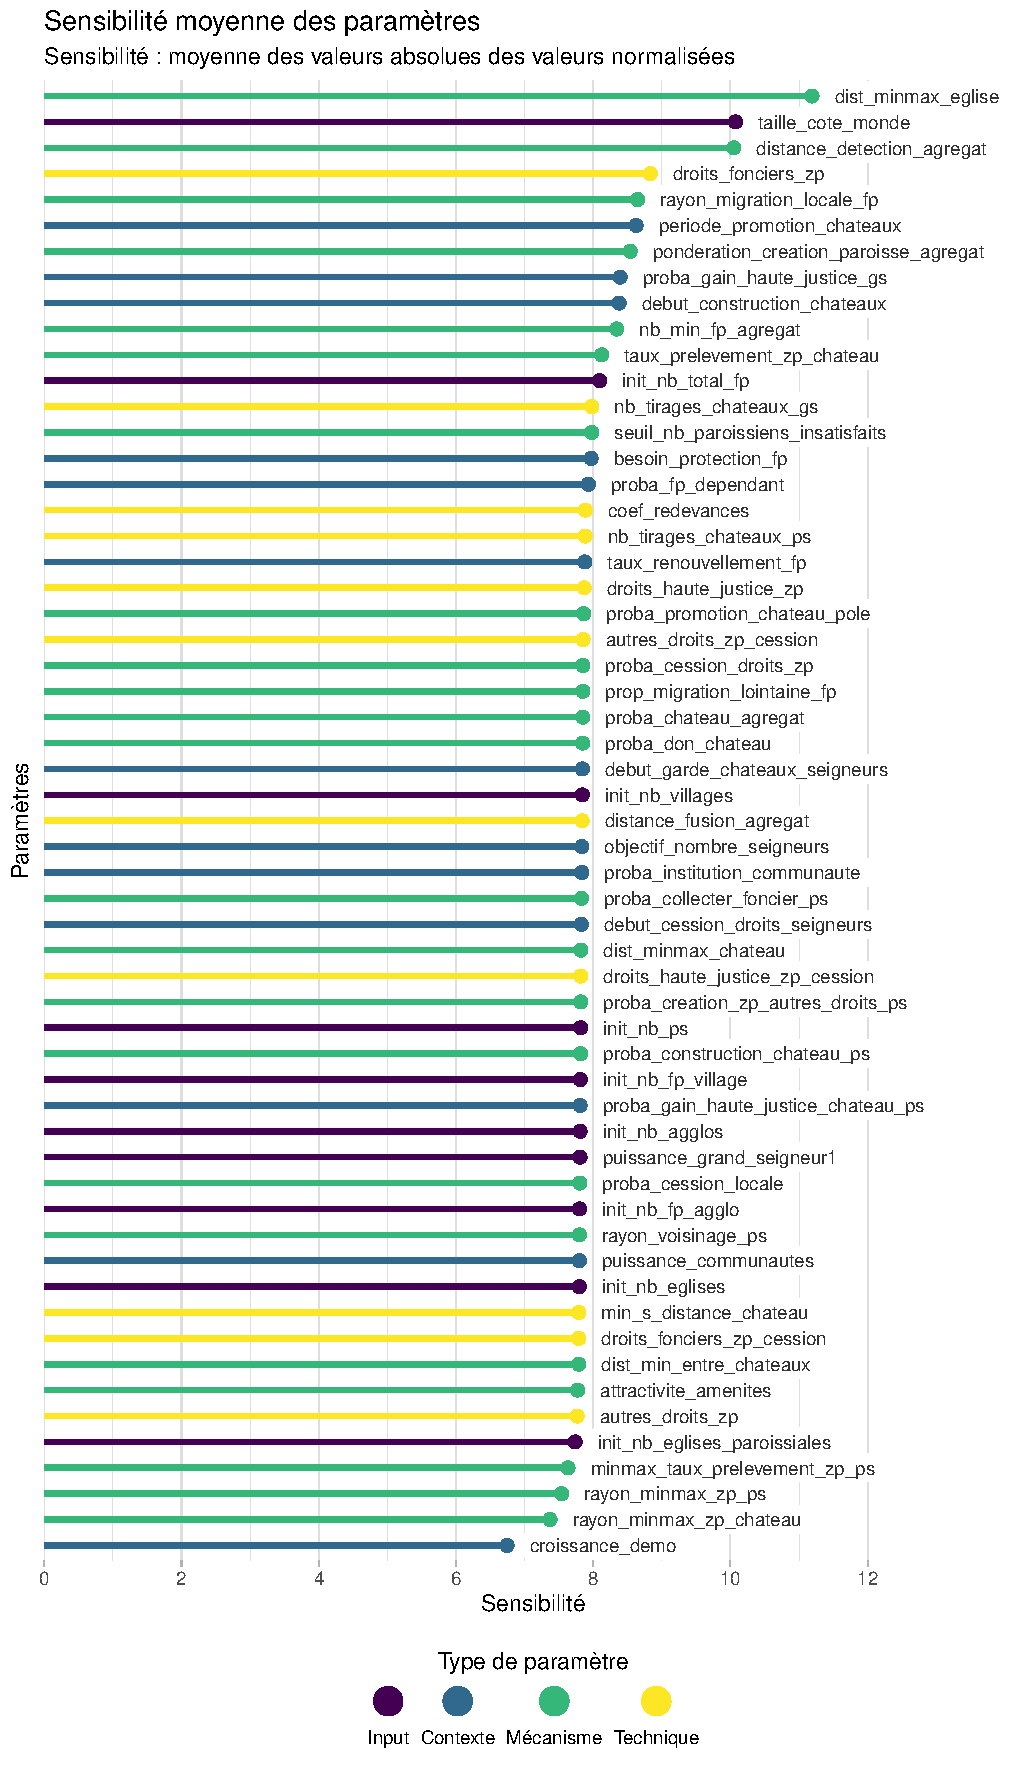
\includegraphics[width=\linewidth]{img/sensibilite_globale.pdf}
	\caption{Analyse de la sensibilité d'ensemble de tous les paramètres de SimFeodal.}
	\label{fig:sensibilite-globale}
\end{figure}

La \cref{fig:sensibilite-globale} présente les \og scores de sensibilité\fg{} de chacun des paramètres du modèle.

Une première remarque est que de manière légèrement contre-intuitive, on ne peut discerner de motif particulier selon les types de paramètres : les \textit{inputs}, paramètres de contexte, de mécanisme et enfin les paramètres techniques sont dispersés et entremêlés dans le graphique.
On se serait vraisemblablement attendu à ce que les inputs et paramètres de contexte jouent un rôle plus important que les paramètres techniques par exemple.

Pondérons toutefois cette remarque en rappelant que malgré une homogénéisation des valeurs en sortie par leur normalisation, il n'y a ici aucune compensation de l'étendue très variable des valeurs de paramètre testées (\hl{disponibles dans l'annexe N}).
Par exemple, si l'on compare un paramètre très sensible (la taille du monde simulé, \textsf{taille\_cote\_monde}) et un paramètre peu sensible (le taux de croissance démographique introduit dans le modèle, \textsf{croissance\_demo}), on peut réaliser que l'ordre de grandeur de la variation est faible.
\begin{itemize}[noitemsep,nolistsep]\vspace*{-.5em}
	\item Pour \textsf{taille\_cote\_monde}, dont la valeur de base est de 80 km, les valeurs testées sont 50, 75, 100, 125 et 150 km.
	Il y a donc à peu près une variation qui va de la moitié de la valeur de base à son double.
	\item Pour \textsf{croissance\_demo}, les seuils sont plus restreints.
	Pour ne pas déstabiliser les autres indicateurs, ce paramètre a été modifié en tenant compte d'une population finale stable de 40 000 foyers paysans, en adaptant à chaque valeur de croissance démographique une valeur différente de population initiale.
	De ce fait, la valeur de base de croissance démographique est de 0\%, et les valeurs testées sont de 1.53\%, 3.72\%, 5.89\% et 12.89\%.
	Ces valeurs permettent de faire passer la population de la stabilité au décuplement. Au regard du paramètre précédent, l'étendue interprétée est large, mais en absolu, les 4 premières valeurs sont très proches et on ne s'attend ainsi pas à ce qu'elles aient un effet majeur sur les sorties du modèle.
\end{itemize}

Un autre exemple de ces étendues incomparables permet d'éclairer la première remarque quant au fait que les paramètres techniques ne sont pas relégués en bas de ce graphique.
Par définition, les paramètres techniques ont des valeurs qui ne représentent strictement rien d'un point de vue thématique.
Leur étendue acceptable est alors extrêmement difficile à évaluer, et on aura ainsi pu avoir tendance à effectuer de mauvais jugements sur les valeurs testées de ces paramètres, les conduisant soit à être sur-valués (le paramètre de caractérisation des droits fonciers, \textsf{droits\_fonciers\_zp} semble entrer dans cette catégorie avant examen spécifique), soit à sembler sous-valués (le paramètre \textsf{distance\_fusion\_agregat} par exemple, a été modifié à de nombreuses reprises lors du paramétrage du modèle et était à ce moment assez important).

Notons aussi que dans les 10 paramètres jugés les plus sensibles, 4 portent sur des valeurs testés \og qualitatives\fg{} (étendues, variables au cours du temps\ldots, voir p.~\pageref{par:etendue-parametres}), alors que ces paramètres ne représentent que 20\% de l'ensemble des paramètres testés.
Là encore, on peut estimer que cette légère sur-représentation de ces paramètres tient à la difficulté de leur attribuer des étendues comparables.

Un dernier constat, à l'échelle très agrégée qui caractérise ces analyses, nous paraît extrêmement rassurant en termes de validation interne du modèle : aucun des paramètres testés ne présente une sensibilité véritablement faible, qui plus est en considérant que la plus faible sensibilité mesurée (paramètre \textsf{croissance\_demo}) correspond à un paramètre dont l'on sait qu'il a une influence réelle sur les sorties du modèle.
Ce simple constat nous indique que dans la limite du jeu de paramètre issu du calibrage, aucun paramètre n'est inutile, et ne devrait par conséquent être supprimé du modèle si on recherchait une parcimonie plus importante à cette étape.



À la lecture du graphique, on remarque qu'autour des 10 premiers paramètres, on peut constater qu'un \og saut\fg{} dans les valeurs de sensibilité se produit entre les paramètres \textsf{nb\_min\_fp\_agregat} et \textsf{taux\_prelevement\_zp\_chateau}.
L'écart entre ce dernier paramètre et le suivant est en effet assez faible, et on décide de ne conserver que les 10 premières paramètres (le 10ème est \textsf{nb\_min\_fp\_agregat}) pour l'analyse visuelle.

La sélection des trois paramètres ayant la plus forte sensibilité sur chaque indicateur complète cette liste avec 4 nouveaux paramètres, portant le total à 14 paramètres dont la sensibilité sera analysée visuellement.
Le \cref{tab:selection-parametres-anavis} en présente la liste ainsi qu'une description complète.

\clearpage
\begin{table}[H]
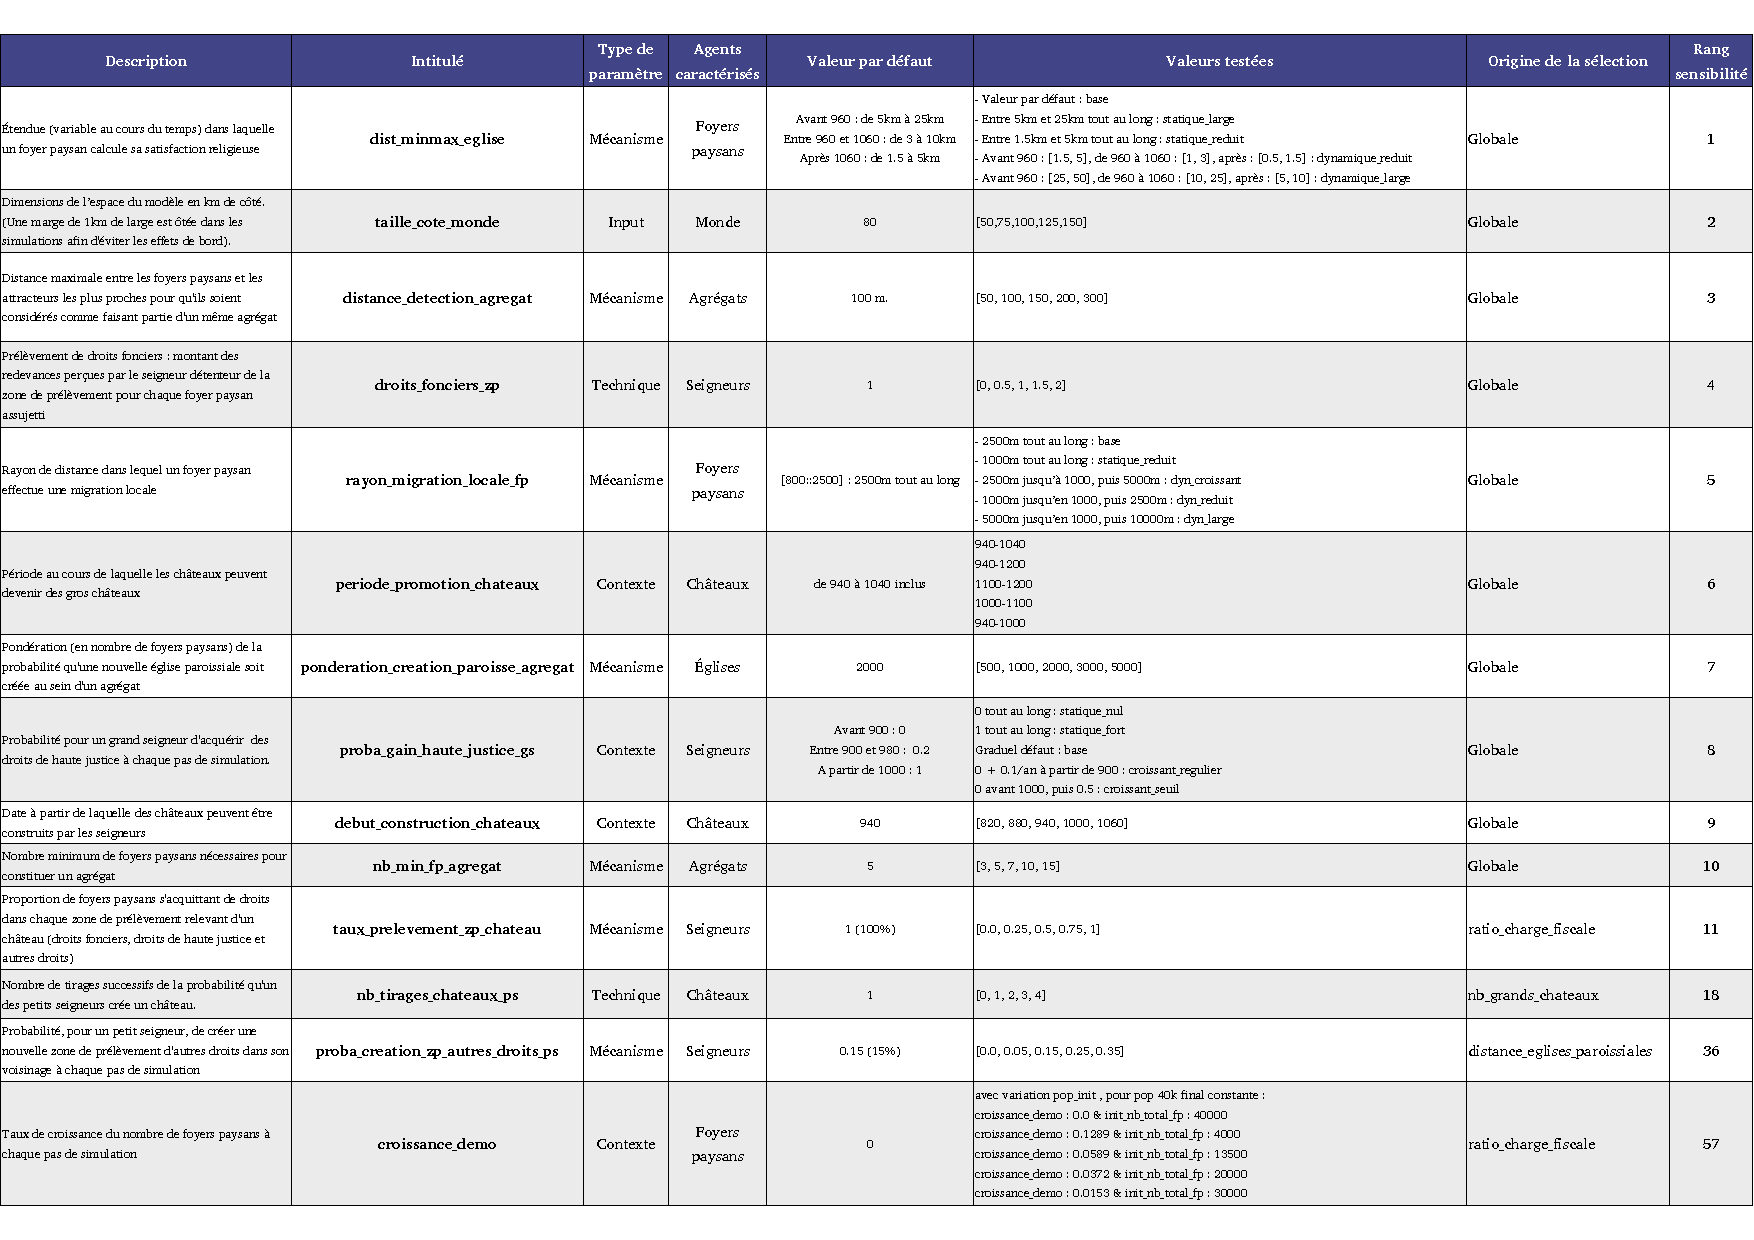
\includegraphics[width=1.75\linewidth, angle=90, origin=c]{img/Parametres.pdf}
\caption{Paramètres sélectionnés pour l'analyse visuelle.}
\label{tab:selection-parametres-anavis}
\end{table}

\subsection{Évaluation visuelle de la sensibilité}

\bigskip
\begin{mdframed}[backgroundcolor=black!5,footnoteinside=false]
	Les graphiques présentés dans la suite de ce chapitre ne concernent que les paramètres sélectionnés lors de l'analyse quantitative globale.
	Tous les paramètres peuvent toutefois être analysés individuellement, de manière interactive, dans la partie dédiée de la plate-forme SimEDB : \hl{Mettre un lien direct}.
\end{mdframed}

Plutôt que de mener l'évaluation de la sensibilité des paramètres sélectionnés de manière linéaire, paramètre après paramètre, nous présentons ces derniers organisés par thématique c'est-à-dire selon les types d'agents concernés par chacun de ces paramètres.

\subsubsection{Monde}

\begin{figure}[H]
	\centering
	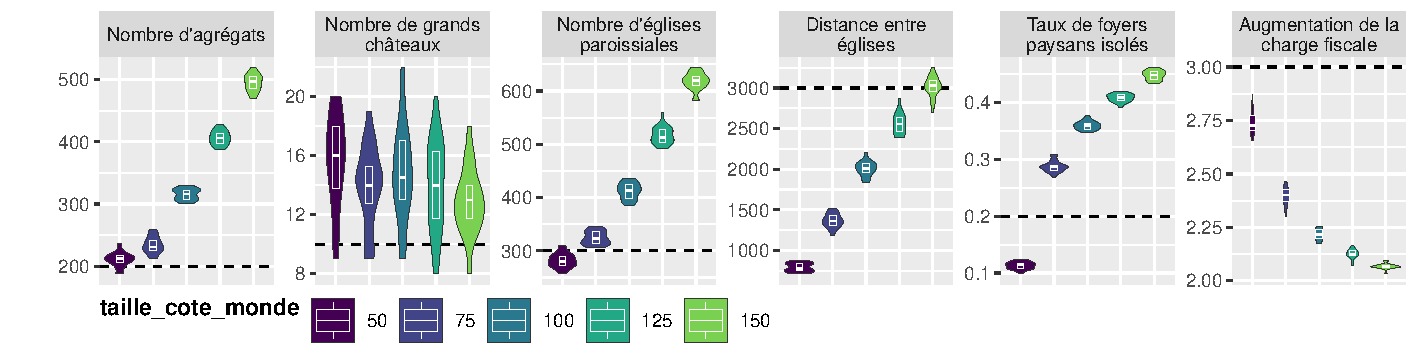
\includegraphics[width=\linewidth]{img/sensib/sensibilite_taille_cote_monde.pdf}
	\caption{Sensibilité à la taille du monde simulé.}
	\label{fig:sensib-monde}
\end{figure}

Le paramètre régissant la taille du monde simulé est le seul des \textit{inputs} présent dans la sélection.
De manière peu surprenante, c'est un paramètre majeur qui affecte la totalité des indicateurs étudiés, selon une polarité assez intuitive (\cref{fig:sensib-monde}).
Plus le monde est restreint, plus les foyers paysans sont proches les uns des autres.
Cela entraîne premièrement une concentration plus forte, mais aussi un nombre d'agrégats plus faible : au lieu d'être dispersés en une multitude de petits agrégats (500 en moyenne avec un monde de 150 km de côté), les foyers paysans se concentrent dans un nombre restreint d'agrégats de superficie vraisemblablement supérieures par les effets des mécanismes de fusion des agrégats.
Quand la superficie d'ensemble est plus faible, toutes choses égales par ailleurs concernant le nombre et le rayon des zones de prélèvement, on assiste nécessairement à une superposition plus importante de ces zones.
La charge fiscale des foyers paysans s'en retrouve fortement affectée.

Un effet de ce paramètre nous paraît légèrement contre-intuitif : avec une surface plus importante, il est entièrement logique que la distance entre les églises augmente, puisque celles-ci sont forcément plus dispersés dans un monde plus large.
Pourtant, le nombre d'églises paroissiales croît aussi avec la superficie du monde simulé, ce qui ne nous semble pas directement interprétable.
On peut émettre l'hypothèse que cette augmentation est une conséquence de la dispersion des foyers paysans au sein de petits agrégats.
De petites églises paroissiales seraient créées ou promues en plus grand nombre dans les zones faiblement peuplées (petits agrégats proches du seuil minimal), là où la création d'une paroisse est moins coûteuse (en termes de nombre de foyers paysans requis) qu'au sein des agrégats plus importants.

\subsubsection{Foyers paysans et agrégats \label{subsubsec:sensib-fp}}

Les foyers paysans (et les agrégats de population qui résultent de leur concentration) sont les agents les plus déterminants dans les l'évolution des structures spatiales observées dans SimFeodal.
À ce titre, il est attendu (et sécurisant en termes de validation interne) que les paramètres contrôlant leurs mécanismes propres aient une influence nette sur les indicateurs de sortie analysés.

Les trois paramètres, spécifiquement liés aux foyers paysans, qui montrent la plus forte sensibilité (\cref{fig:sensib-fp}) embrassent trois aspects bien différent des mécanismes des foyers paysans.

\begin{figure}[H]
	\centering
	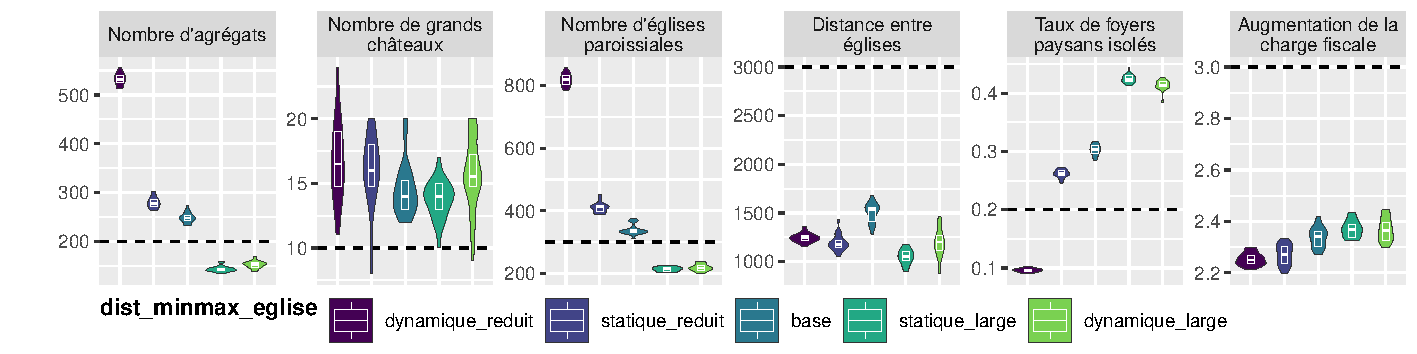
\includegraphics[width=\linewidth]{img/sensib/sensibilite_dist_minmax_eglise.pdf}
	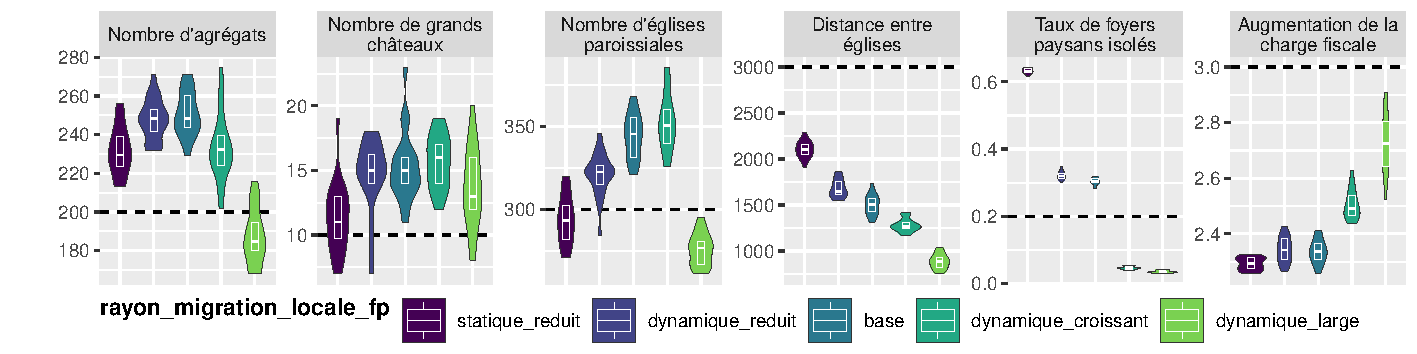
\includegraphics[width=\linewidth]{img/sensib/sensibilite_rayon_migration_locale_fp.pdf}
	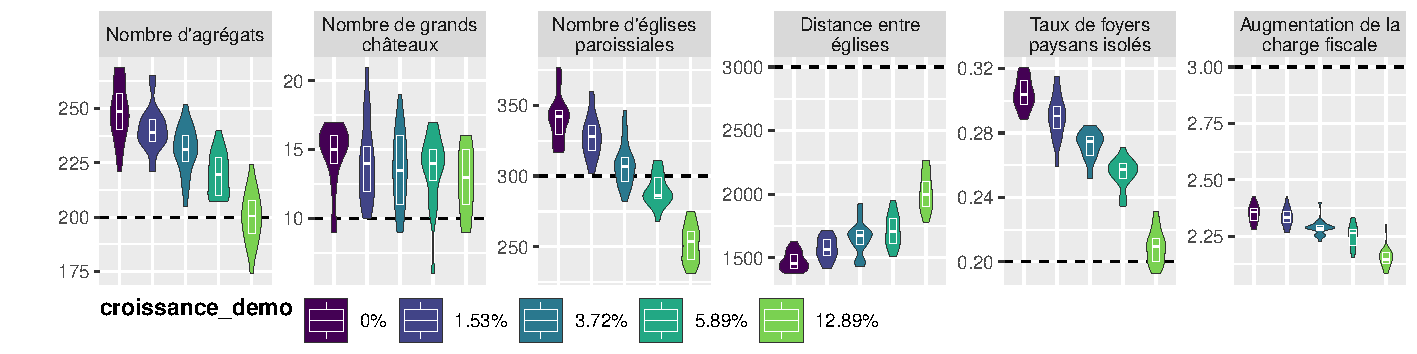
\includegraphics[width=\linewidth]{img/sensib/sensibilite_croissance_demo.pdf}
	\caption{Sensibilité des paramètres liés aux foyers paysans.}
	\label{fig:sensib-fp}
\end{figure}

Le premier de ces paramètres, qui est aussi le plus sensible du modèle, joue sur la satisfaction religieuse des foyers paysans.
Notons déjà que le calibrage de ce paramètre semble efficace : au moins sur les quatre premiers indicateurs, c'est la valeur par défaut dans le modèle qui approche le plus des objectifs.
En matière d'interprétation, le fait que cette satisfaction soit déterminante est inattendu : on a pu constater dans les résultats du modèle (\cref{fig:result-fp-satis}) que le facteur limitant de la satisfaction d'ensemble était la satisfaction protection.
Les valeurs testées, qualitatives, ont une large influence sur les aspects liés à la concentration des foyers paysans, et leur action sur les autres indicateurs est moins linéaire et évidente.
Plus les étendues testées sont restreintes, plus le nombre d'agrégats et de foyers paysans isolés est important : cette satisfaction joue sans doute à ce moment là le rôle limitant et \og force\fg{} les foyers paysans à migrer à proximité d'églises paroissiales.

Cette migration, au moins pour l'aspect local, est largement influencée par le second paramètre de la sélection : le rayon maximal de migration locale des foyers paysans. 
Celui-ci n'est pas une étendue, mais un seuil maximum qui peut (valeurs \og dynamiques\fg{}) changer au cours du temps, la logique étant que plus le temps passe, plus ce rayon est susceptible d'augmenter en lien avec des aspects cognitifs et liés à l'intégration du système de peuplement qui voit ses distances-temps rétrécir.
Ce paramètre a notamment un rôle déterminant sur la concentration des foyers paysans, puisque selon les valeurs éprouvées, cet indicateur peut passer en moyenne de 63\% à seulement 3\%.
Les effets sur le nombre d'agrégats, de grands châteaux et d'églises paroissiales ne sont pas directement linéaires et l'on peut penser que les variations de ce paramètre montre alors des tendances diverses selon l'ordre de grandeur des seuils empruntés.

La croissance démographique est particulière dans le modèle.
On la considère comme un paramètre de contexte, mais elle aurait également entièrement sa place parmi les \textit{inputs} tant son importance thématique est majeure.
À la lecture des graphiques, on peut s'étonner de ce que ce paramètre soit le moins sensible (\cref{fig:sensibilite-globale}) tant son effet est direct sur tous indicateurs présentés (à l'exception du nombre de grands châteaux).
On remarque qu'un taux de croissance plus élevé réduit le nombre d'agrégats tout en réduisant aussi le taux de foyers paysans isolés, deux effets qui sont souvent inverses dans les différents paramètres.
C'est extrêmement intéressant pour le modèle tant ce paramètre permet d'approcher des objectifs de ces indicateurs qui sont tous deux dépassés alors qu'opposés.
Ce paramètre fait l'objet d'un scénario thématique (\cref{subsec:scenario-croissance}), et on le décrira plus avant à ce moment-là.


\begin{figure}[H]
	\centering
	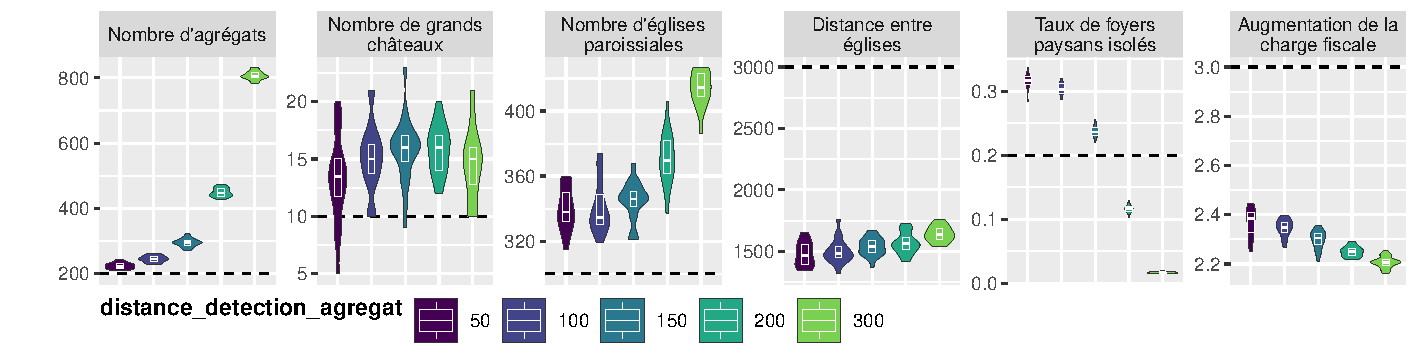
\includegraphics[width=\linewidth]{img/sensib/sensibilite_distance_detection_agregat.pdf}
	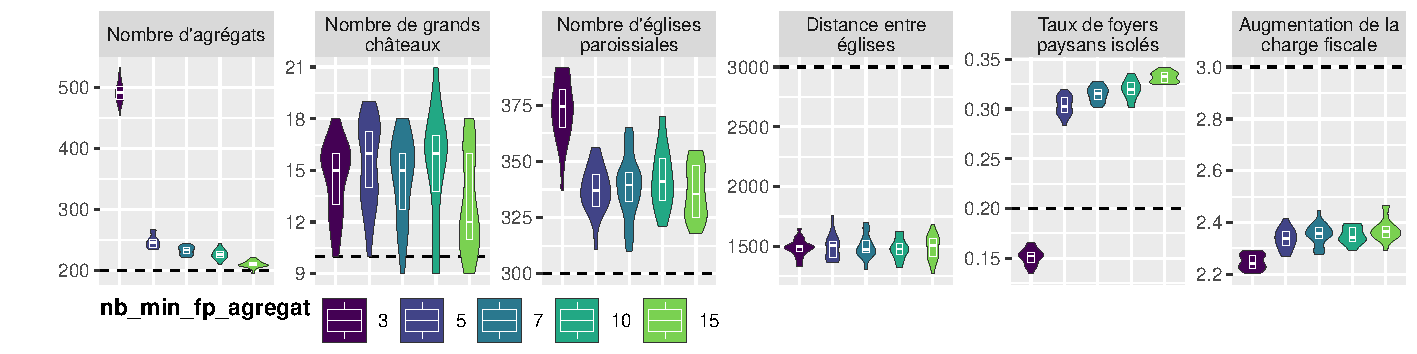
\includegraphics[width=\linewidth]{img/sensib/sensibilite_nb_min_fp_agregat.pdf}
	\caption{Sensibilité des paramètres liés aux agrégats.}
	\label{fig:sensib-agregats}
\end{figure}

Les deux paramètres agissant sur la définition des agrégats (\cref{fig:sensib-agregats}) sont très comparables et agissent de manière symétriquement opposée sur les indicateurs de sortie.
Sans surprise, leur effet est largement circonscrit aux indicateurs relatifs aux foyers paysans (à l'exception surprenant des églises paroissiales, peut-être pour les mêmes raisons que le paramètre de taille du monde simulé), mais il est intéressant de noter leur extrême sensibilité, plus que linéaire, à des variations relativement fines dans les ordres de grandeur mobilisés (quelques foyers paysans de plus à l'échelle des 40 000, 50 ou 100 mètres à l'échelle d'un monde de 80 kilomètres de côté\ldots).
Les variations présentées dans la figure indique que les valeurs par défaut (100 m et 5 foyers paysans) sont au moins dans des intervalles assez sensées au regard des objectifs poursuivis.

\subsubsection{Seigneurs et châteaux}

Les paramètres liés aux seigneurs et aux châteaux (les premiers construisant les seconds) sont les plus nombreux du modèle et il est attendu qu'ils soient assez sensibles : ce sont les mécanismes associés qui façonnent le monde dans lequel les foyers paysans auront à évoluer et dans lequel ils essaieront de ne pas être trop insatisfaits.

\begin{figure}[H]
	\centering
	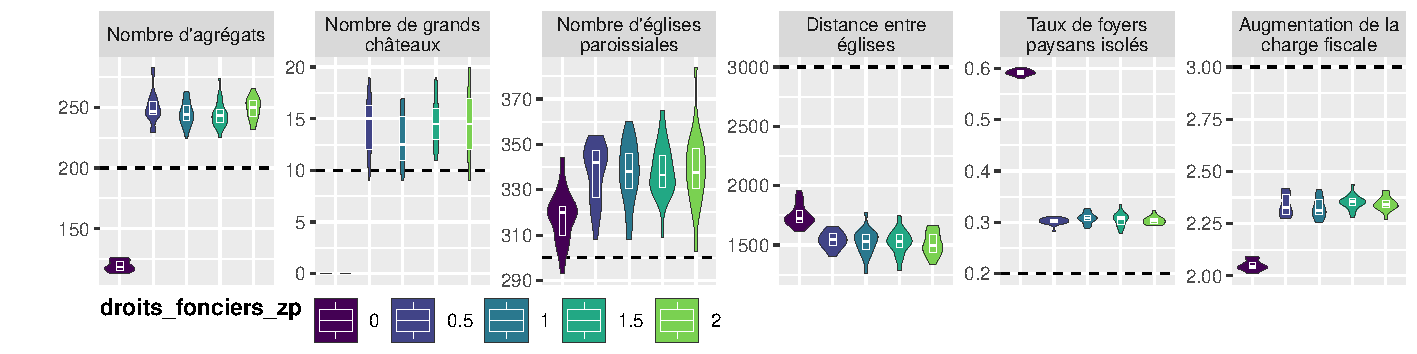
\includegraphics[width=\linewidth]{img/sensib/sensibilite_droits_fonciers_zp.pdf}
	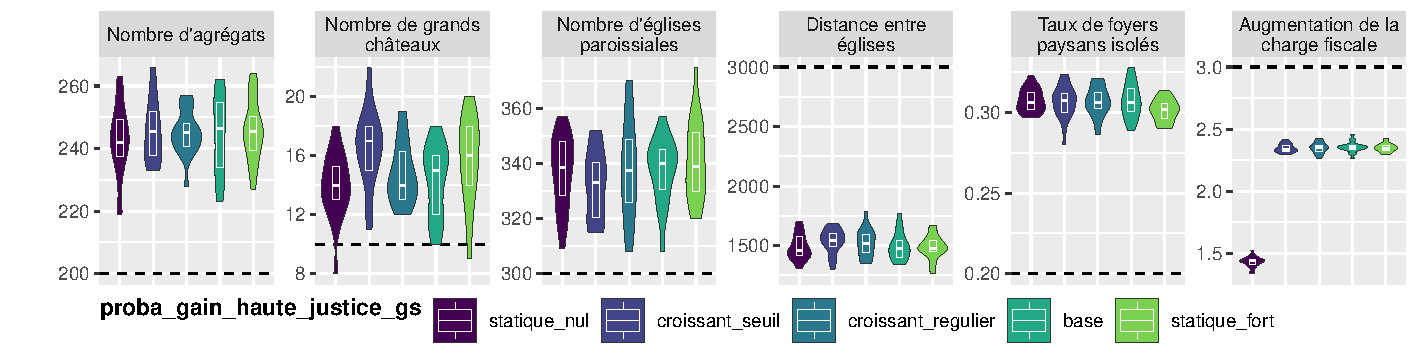
\includegraphics[width=\linewidth]{img/sensib/sensibilite_proba_gain_haute_justice_gs.pdf}
	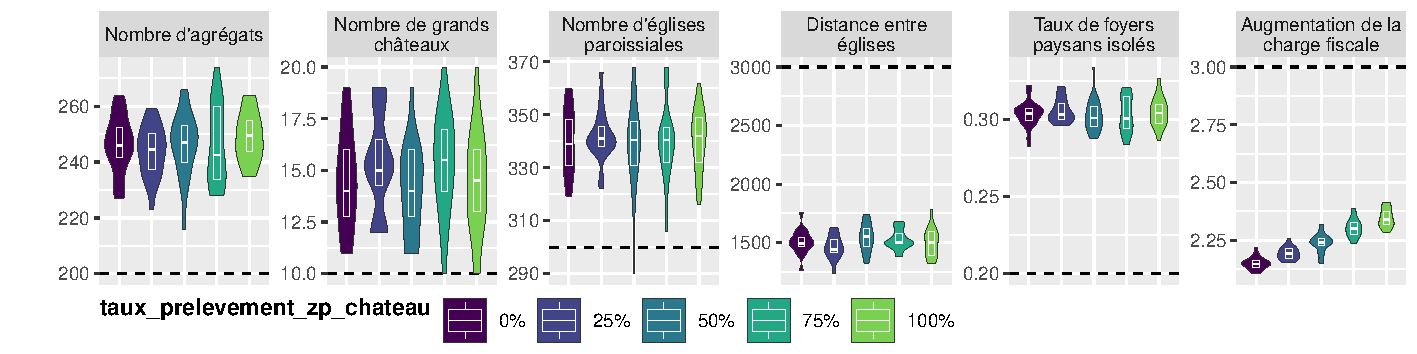
\includegraphics[width=\linewidth]{img/sensib/sensibilite_taux_prelevement_zp_chateau.pdf}
	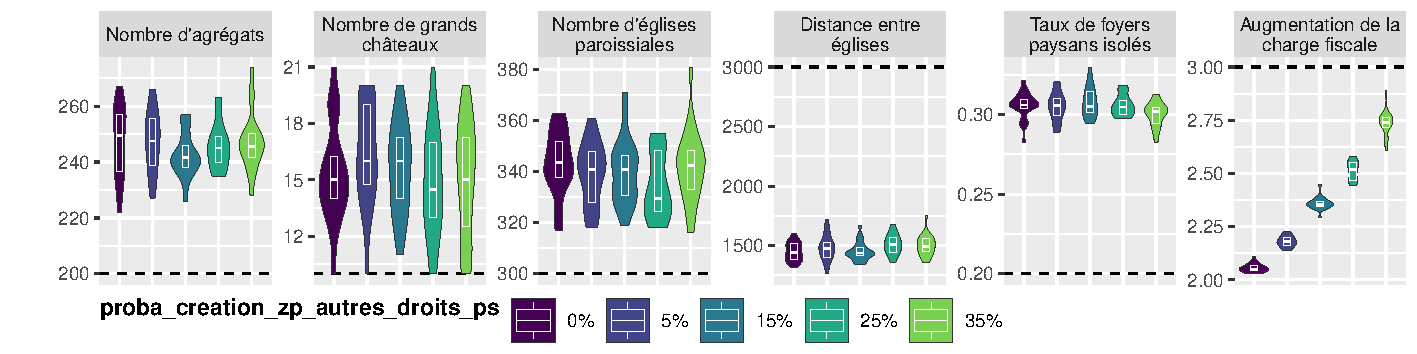
\includegraphics[width=\linewidth]{img/sensib/sensibilite_proba_creation_zp_autres_droits_ps.pdf}
	\caption{Sensibilité des paramètres liés aux seigneurs.}
	\label{fig:sensib-seigneurs}
\end{figure}

Une caractéristique commune aux quatre paramètres isolés (\cref{fig:sensib-seigneurs}) tient au test de valeurs nulles, ou autrement dit, à la désactivation des mécanismes associés.
Dans les deux premiers paramètres, l'effet de rupture est net, par exemple sur l'augmentation de la charge fiscale.
Le montant des droits fonciers collectés ne joue que par son activation ou non (les valeurs supérieures à 0 présentent des résultats très similaires), mais présente un effet clair sur le nombre d'agrégats et l'agrégation des foyers paysans.
L'existence et la propension des droits de haute justice des grands seigneurs ne semble jouer que sur la charge fiscale, mais y exerce une influence énorme : c'est le seul paramètre dont une valeur testée peut faire diminuer autant (1.5 alors que l'ordre de grandeur des simulations est plutôt entre 2 et 2.5)

Il est intéressant de remarquer que pour les deux paramètres suivant, où la valeur de 0\% correspond aussi à une désactivation du mécanisme lié, cela n'a aucun effet de seuil notable : ces paramètres se comportent, dans l'étendue testée, comme des éléments linéaires sur l'augmentation de la charge fiscale.
Ils semblent assez dépourvus d'influence sur les autres indicateurs, mais en particulier pour le dernier paramètre, leur action sur la charge fiscale est notable.
Pour améliorer le calibrage du modèle sur cet indicateur, on aurait sans doute intérêt à augmenter la valeur par défaut du paramètre \textsf{proba\_creation\_zp\_autres\_droits\_ps}, y compris au delà des valeurs ici testées.
Ce serait d'autant plus adapté que la sensibilité globale de ce paramètre est relativement faible (36ème sur les 57 paramètres).


\begin{figure}[H]
	\centering
	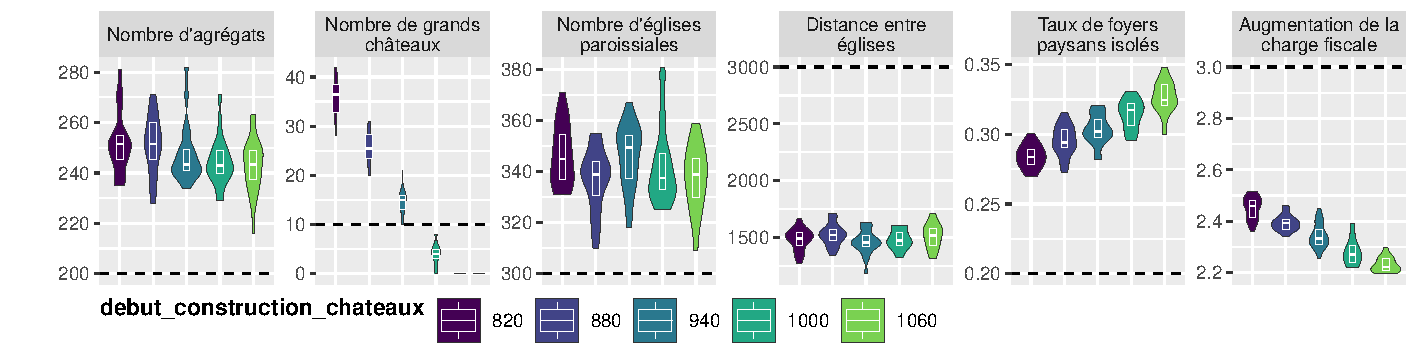
\includegraphics[width=\linewidth]{img/sensib/sensibilite_debut_construction_chateaux.pdf}
	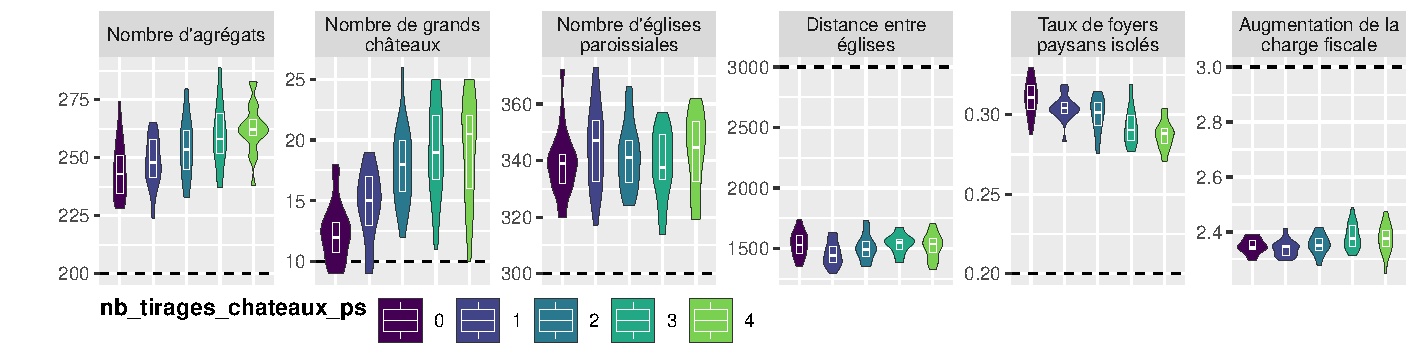
\includegraphics[width=\linewidth]{img/sensib/sensibilite_nb_tirages_chateaux_ps.pdf}
	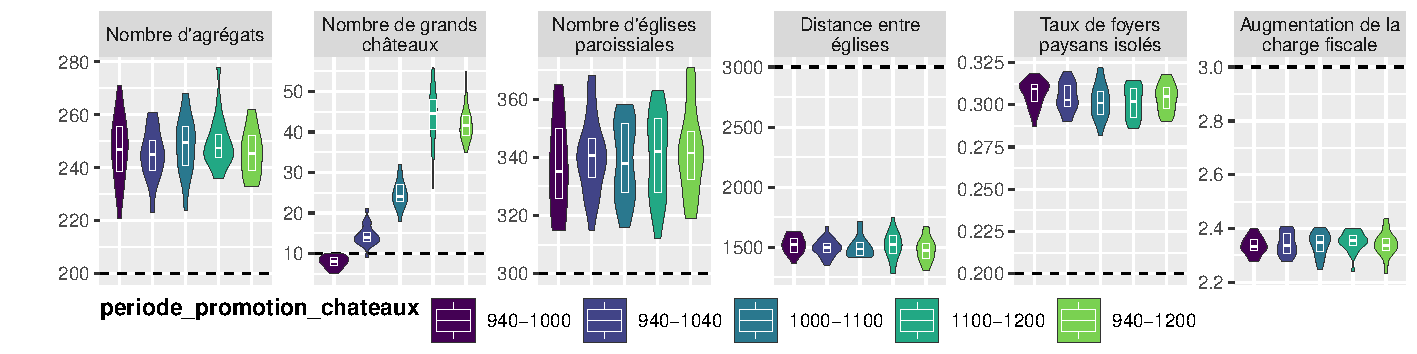
\includegraphics[width=\linewidth]{img/sensib/sensibilite_periode_promotion_chateaux.pdf}
	\caption{Sensibilité des paramètres liés aux châteaux.}
	\label{fig:sensib-chateaux}
\end{figure}

Les paramètres liés aux châteaux sont sensiblement sur-représentés parmi ceux qui ont la sensibilité la plus forte : il n'y en a que 6 sur les 57 paramètres (environ 11\%), mais ils représentent 20\% des paramètres les plus sensibles et 21\% dans cette sélection de paramètres remarquables .

C'est assez remarquable, d'autant qu'on peut constater à la lecture des deux premiers paramètres de la (\cref{fig:sensib-chateaux}) que leur rôle ne se cantonne absolument pas à un simple raffinement du contexte où l'atteinte d'un certain nombre de grands châteaux serait à la fois un objectif et un élément déterministe.
Sur ces deux premiers paramètres, on remarque certes une très forte variation de l'indicateur directement lié, le nombre de grands châteaux, mais aussi et surtout un lien net avec la concentration des foyers paysans (et un autre lien moins significatif avec l'augmentation de la charge fiscale).
La conception et le paramétrage des mécanismes liés aux châteaux ont demandé un travail conséquent (voir la partie dédiée leur calibrage -- \cref{subsec:calibrage} -- p.~\pageref{subsubsec:calibrage-chateaux}), vraisemblablement trop important relativement à la complexité de leurs règles et à notre propre estimation subjective de leur apport concret au modèle.
Pourtant, les résultats de cette analyse de sensibilité donnent tort à l'expertise du modélisateur et gain de cause aux thématiciens pour lesquels les châteaux, et la justesse de leur implémentation, avaient une dimension thématique considérable.
La portée réduite mais claire de ces paramètres sur le premier objectif thématique recherché (la concentration des foyers paysans) justifie de leur existence et de leur nécessité dans les processus modélisés au sein de SimFeodal.

Le troisième paramètre, la période durant laquelle les châteaux peuvent être promus en grands châteaux, apporte un léger contrepoint, ou au moins une précision à ce constat.
Ce paramètre est déterminant dans le nombre de grands châteaux présents en fin de simulation, mais pourtant, il n'a aucune influence significative sur les autres indicateurs.
Peut-on dès lors penser que la hiérarchie mise en place entre les châteaux, et la différence d'attractivité qui en découle, n'est pas indispensable au modèle ?
Il faudra pour cela mener une étude plus approfondie des relations entre proportion de grands châteaux et les autres indicateurs.
Rappelons en effet que l'analyse de sensibilité ici menée est grossière, et n'étudie aucunement les interactions entre valeurs de paramètres dont on peut imaginer, au sein d'un modèle aussi descriptif et complexe, qu'ils ont des effets locaux conséquents.

\subsubsection{Églises et paroisses}

Le dernier paramètre de cette analyse visuelle est aussi le seul qui porte sur un élément aussi conséquent que les paroisses, lesquelles sont l'un des moteurs principaux de la fixation de la population dans les agrégats de taille réduite qui constituent la grande majorité des lieux de concentration des foyers paysans (la fameuse \og longue traîne\fg{} de cette hiérarchie).

\begin{figure}[H]
	\centering
	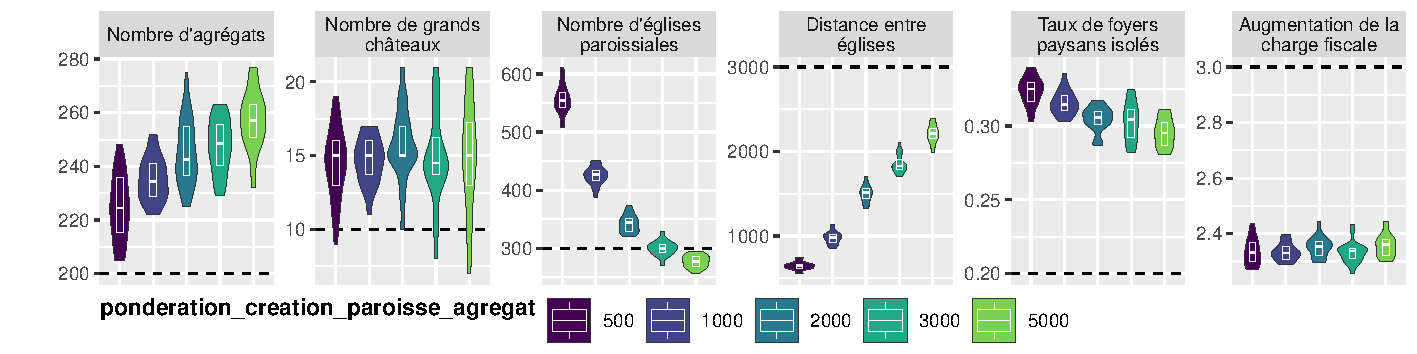
\includegraphics[width=\linewidth]{img/sensib/sensibilite_ponderation_creation_paroisse_agregat.pdf}
	\caption{Sensibilité du paramètre de pondération de création de nouvelles paroisses dans les agrégats.}
	\label{fig:sensib-paroisses}
\end{figure}

La \cref{fig:sensib-paroisses} présente les réponses des indicateurs à différentes valeurs du paramètre \textsf{ponderation\_creation\_paroisse\_agregat}.
De manière prévisible et évidente, ce paramètre influence nettement les deux indicateurs liés aux paroisses et églises.
Plus grand est le nombre de paroissiens nécessaire à la création d'une nouvelle paroisse dans un agrégat, plus faible est le nombre d'églises paroissiales conséquemment créées.
Et moins il y a d'églises dans un monde à la superficie constante, plus large est la distance entre elles.
Passé cette trivialité, on notera avec intérêt la variation amenée par ce paramètre sur le nombre d'agrégats : plus le seuil est élevé, plus les agrégats sont nombreux, et cette corrélation apparaît visuellement significative et inverse à celle du nombre d'églises paroissiales, contrairement aux tendances que l'on a pu observer dans les paramètres liés aux foyers paysans et agrégats (\cref{subsubsec:sensib-fp}).
Avec ces paramètres, nombre d'agrégats et d'églises paroissiales varient dans le même sens face aux valeurs de paramètres.
Dans le cas du paramètre de pondération de la création de paroisses \og urbaines\fg{}, la relation est inverse, et il est difficile de l'expliquer, de même que le lien (plus ténu, mais lui aussi inverse) avec la concentration des foyers paysans.
On peut émettre l'hypothèse que cette pondération influe largement sur la hiérarchie des paroisses et des pôles.
En créant moins de paroisses en zone dense, la distribution de l'attractivité des pôles d'attraction -- qui est mesurée en large partie sur le nombre d'églises paroissiales qui les composent -- tend peut-être vers plus d'uniformité, et favorise ainsi relativement l'attraction locale vers des pôles de plus faible attractivité, et donc vers des agrégats plus locaux et faiblement peuplés.



\subsection{Analyser la sensibilité à l'aléa}

En menant l'analyse de sensibilité visuelle, on a pu remarquer que certains indicateurs présentaient une plus forte variation que d'autres.
Une partie de l'explication tenait certainement à l'inégale amplitude des valeurs de paramètres testées, lesquelles influencent potentiellement plus directement ces indicateurs, mais cela ne nous semble pas être une explication suffisante.

De manière globale, on constate dans les résultats de la version calibrée de SimFeodal (\cref{tab:results-basique}) que la variabilité des indicateurs émergents est assez forte en termes d'écart-type.
L'écart-type se lisant dans l'unité de l'indicateur mesuré, il peut être intéressant de le transformer en coefficient de variation ($CV_{\text{indicateur}} = \sigma_{\text{indicateur}}  /  \mu_{\text{indicateur}}$) pour obtenir des valeurs comparables entre les indicateurs. 


\begin{table}[H]
{\renewcommand{\arraystretch}{1.1}%
	\begin{tabular}{|p{5cm}|p{2.5cm}|p{2.5cm}|p{2.5cm}|}
\hline
\textbf{Indicateur} & \textbf{Moyenne} & \textbf{Écart-type} & \textbf{Coefficient de variation} \\
\hline
\textit{Agrégats} & 249 & 10.45 & 0.042\\
\hline
\textit{Grands châteaux} & 15 & 2.87 & 0.191\\
\hline
\textit{Églises paroissiales} & 348 & 12.96 & 0.037\\
\hline
\textit{Distance moyenne entre églises} & 1459 m & 97 m & 0.066\\
\hline
\textit{Part de foyers paysans isolés} & 30\% & 0.8 \% & 0.027\\
\hline
\textit{Augmentation de la charge fiscale des foyers paysans} & $\times$ 2.4 & 0.030 & 0.013\\
\hline
\multicolumn{3}{r|}{\textbf{\textit{Moyenne}}} & 0.063\\
\cline{4-4}
	\end{tabular}
}
\caption{Mesures de dispersion des indicateurs de sortie de la version calibrée (6.6) de SimFeodal.}
\label{tab:variabilite-indicateurs}
\end{table}

La lecture du \cref{tab:variabilite-indicateurs} nous montre que, rapportée à un paramètre de dispersion relatif comme le coefficient de variation, la variabilité des indicateurs due à l'aléa est assez faible, et dans des ordres de grandeurs assez comparables entre les indicateurs (à l'exception du nombre de grands châteaux).

Pourtant, lors de l'analyse de sensibilité, on a pu constater des variations (étendue dans l'axe des ordonnées des \textit{violin-plots}) bien plus importantes au sein des réplications des paramètres testés.

Il nous paraît par conséquent utile de mener un bref complément d'analyse, dédié à l'étude de la variabilité au sein des réplications d'une expérience.
De telles analyses nous paraissent peu fréquentes dans la littérature liée aux modèles de simulation en géographie, mais on en trouve tout de même une définition chez \textcite{ginot2005explorer}, qui nomment ces approches des \og analyses d'incertitude\fg{} : 
\begin{quotation}
	\og Compte tenu des incertitudes sur les paramètres, de la variabilité naturelle des variables d'entrée et des composantes stochastiques qui peuvent être incluses dans la structure du modèle, il s'agit de calculer l'incertitude associée aux variables de sorties.
	Les analyses d'incertitude sont très liées aux analyses de sensibilité dans la mesure où l'on souhaite en général connaître non seulement cette incertitude, mais également son origine.
	C'est pourquoi ces deux types d'analyses sont souvent menées en parallèle, voire confondues.\fg{}\\
	\mbox{}~ \hfill \cite[76]{ginot2005explorer}
\end{quotation}

Pour mesurer cette incertitude, nous avons repris l'ensemble des réplications correspondant à l'analyse de sensibilité de chaque paramètre, en avons mesuré la variabilité (écart-type) sur chaque indicateur.
Afin à nouveau d'avoir des mesures comparables, on a ensuite procédé à une réduction (division par l'écart-type des valeurs de référence, présentées dans le \cref{tab:variabilite-indicateurs}) de l'amplitude de ces valeurs.

\begin{figure}[H]
	\centering
	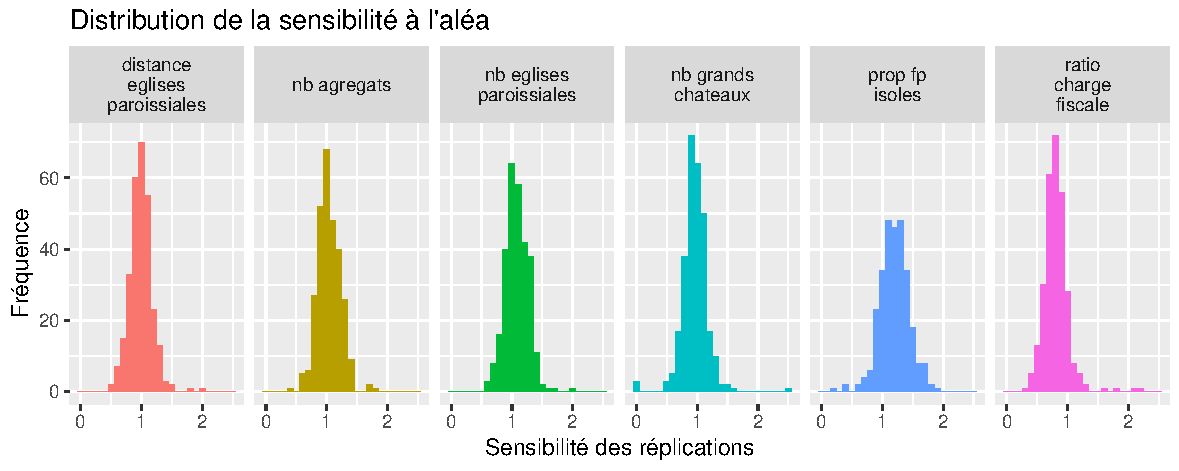
\includegraphics[width=\linewidth]{img/histo_sensibilite_alea.pdf}
	\caption{Sensibilité à l'aléa selon les indicateurs.}
	\label{fig:histo-sensib-alea}
\end{figure}

La distribution de ces valeurs d'incertitude réduites est présenté dans la \cref{fig:histo-sensib-alea}.
Dans ces histogrammes, la valeur de 1 correspond à une incertitude moyenne identique à celle des réplications de référence.
Une valeur de 2 peut être comprise ainsi : pour l'indicateur considéré, les différentes simulations exécutées lors de l'analyse de chaque valeur de chaque paramètre ont une variabilité deux fois supérieure à la variabilité attendue.
Autrement dit, certaines valeurs de certains paramètres amènent une bien plus forte variabilité : ils laissent une part plus importante à la stochasticité du modèle.

On peut remarquer que la plupart des indicateurs présentent des \textit{outliers}, c'est-à-dire des valeurs de paramètres pour lesquelles la variabilité due à l'aléa est nettement supérieure (ou inférieure) à la normale.
Dans le cas du nombre de grands châteaux, il y a même des valeurs de paramètres qui montre une absence presque totale de variabilité à l'aléa.
Sans aller plus loin sur cet exemple, on peut penser qu'il s'agit des valeurs de paramètre qui ont tendance à réduire très largement le nombre de châteaux, amenant alors à une variabilité extrêmement faible dans cette amplitude des possibles restreinte.

À partir de cet histogramme, nous avons isolés les \textit{outliers} et en présentons une représentation graphique dans la \cref{fig:sensib-alea}.
\begin{figure}[H]
	\centering
	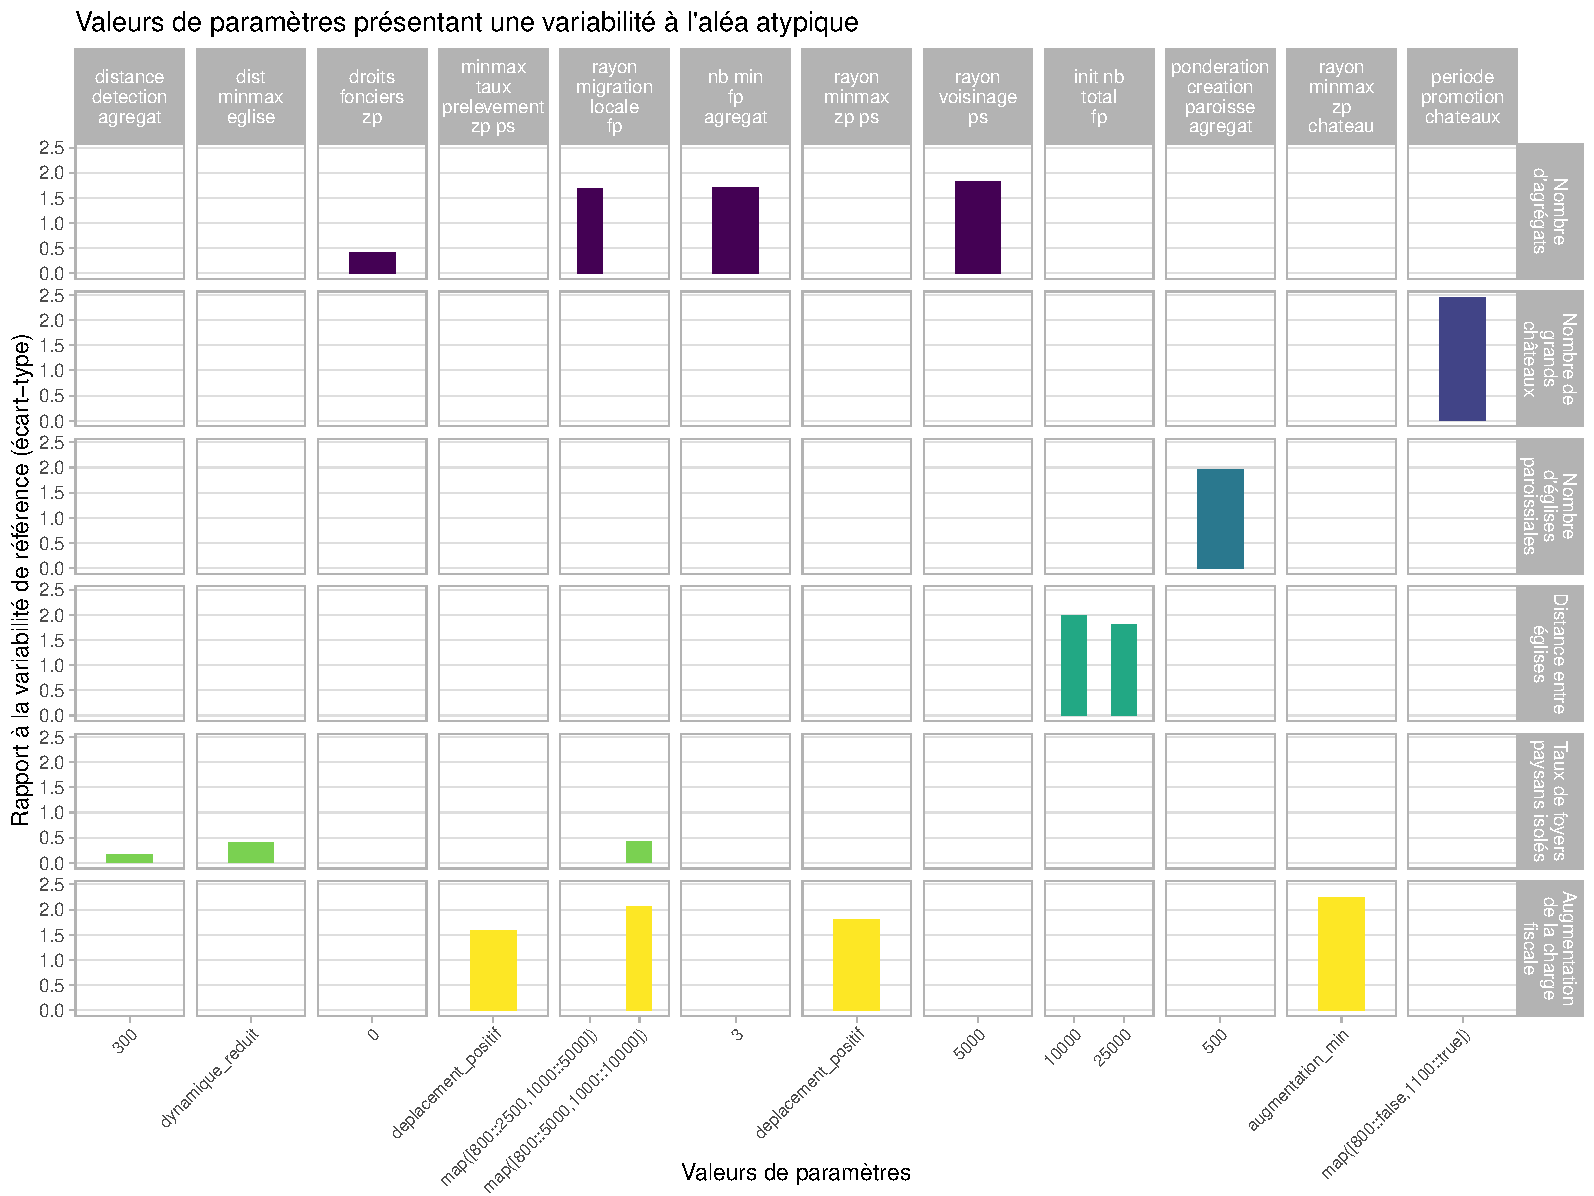
\includegraphics[width=\linewidth]{img/sensibilite_alea_outliers.pdf}
	\caption{Paramètres présentant des sensibilités atypiques à l'aléa.}
	\label{fig:sensib-alea}
\end{figure}

De manière globale, on peut remarquer que les indicateurs relatifs aux foyers paysans présentent plus de valeurs extrêmes que les autres, c'est-à-dire sur une plus forte diversité de paramètres.
Notons aussi que sur les 14 valeurs de paramètres isolées, la moitié concernent des paramètres qualitatifs.
La difficile estimation de l'amplitude ceux-ci explique sans doute en partie la plus forte variabilité à l'aléa : si on a choisit des valeurs (étendues, évolutions temporelles etc.) trop éloignées des valeurs calibrées, il se peut que le modèle passe dans des régimes locaux différents du régime de base caractérisé par les réponses aux paramètres calibrés.

Plus spécifiquement, on peut constater le comportement très particulier du paramètre régissant le rayon maximum de migration locale des foyers paysans.
Non seulement les valeurs de ce paramètre sont parmi les plus fortes sensibilités à l'aléa (indicateurs nombre d'agrégats et augmentation de la charge fiscale), mais de manière surprenante, la valeur correspondant à un rayon évolutif très étendue par rapport à la valeur de base (\texttt{map([800:5000, 1000:10000])}) se caractérise aussi par une très faible sensibilité à l'aléa sur l'indicateur de concentration des foyers paysans.
Ce paramètre a donc la capacité de faire fortement varier les sorties (vu dans l'analyse de sensibilité visuelle), mais en plus de varier tout aussi fortement la part de l'aléa dans le modèle.
Nous pensions exécuter un scénario thématique qui fasse varier ce paramètre afin d'étudier l'effet sur la hiérarchie des agrégats, et cette analyse confirme que ce serait tout à faire approprié.

\subsection{Conclusion et apports de l'analyse visuelle de sensibilité}

On peut tirer un bilan extrêmement positif de l'exécution de cette analyse de sensibilité, pourtant limitée et grossière.

Dans un premier temps, notons que la hiérarchie de la sensibilité des paramètres n'est pas véritablement proche de celle que l'on attendait, et qu'on a sans doute agit lors du paramétrage et du calibrage sur des paramètres qui n'étaient pas les plus déterminants.
Cette étape d'évaluation qu'est l'analyse de sensibilité aurait sans doute gagné à être menée avant le calibrage du modèle afin d'obtenir une meilleure adéquation aux objectifs.
Ce raisonnement est toutefois circulaire : sur un modèle moins calibré, peut-être que l'analyse de sensibilité n'aurait pas mis en avant les mêmes paramètres.
Ceux-si sont en interaction étroite, et il nous semble évident que les résultats de cette analyse de sensibilité sont eux même extrêmement sensibles au paramétrage de base.

Dans un second temps, l'analyse de sensibilité semble aller dans le sens d'une confirmation de la parcimonie du modèle.
On l'a dit lors de l'analyse quantitative, mais il nous semble important de le répéter tant ce résultat est rassurant, mais aussi surprenant.
Aucun des paramètres n'apparaît inutile, ce qui peut laisser entendre que les (très) nombreux mécanismes du modèle ne le sont pas non plus.
Pour un modélisateur qui pense à minima comprendre à peu près son modèle et a des intuitions fortes sur les réactions de celui-ci aux différents mécanismes et paramètres, c'est une surprise très positive.
Surprise d'autant plus positive que cet examen systématique des paramètres se révèle réellement une aide indéniable à la compréhension du modèle : après plus de 5 ans à travailler régulièrement sur un modèle, il est très enrichissant d'y trouver encore des éléments inattendus.

Un autre point, classique, concerne les limites d'une telle analyse.
L'approche entièrement quantitative, présentée dans l'introduction de cette partie, permet de s'affranchir des effets de mauvaise pondération que l'on a pu constater dans l'analyse visuelle : certains paramètres ont une sensibilité globale importante, mais celle-ci se cantonne parfois à un unique indicateur, sans avoir de répercussions sur le reste du modèle.
Dans un modèle comme SimFeodal, c'est-à-dire descriptif, exploratoire, et composé d'autant de paramètres hétérogènes, il semble toutefois illusoire de réussir à quantifier, pour une analyse de sensibilité, tout ce qui n'a pas été quantifié dans le modèle en lui-même : pondération des objectifs, objectivation des attendus dans les indicateurs graphiques etc.

C'un point de vue subjectif assumé, la démarche mise en place, basée sur le visuel, nous semble tout à fait fructueuse. 
Elle s'inscrit, comme de nombreux aspects de ce travail de thèse, dans une approche d'analyse visuelle entièrement dédiée à l'exploration d'un modèle et paraît confirmer l'adéquation de ce type d'approches à la construction et évaluation commune et interdisciplinaire de modèles.

La dernière partie de ce chapitre, tournée vers l'usage du modèle pour tester des scénarios thématiques, trouve enfin une justification supplémentaire, dans le champ méthodologique et de la modélisation cette fois-ci.
Les brèves analyses de sensibilités ont en effet renforcé le besoin criant d'études plus approfondies des variations de certains paramètres, qui plus est quand ceux-ci trouvent des correspondances dans les connaissances empiriques.

\clearpage
\section[Exploration de scénarios]{Comprendre le modèle par l'exécution de scénarios%
	\sectionmark{Comprendre le modèle par l'exécution de scénarios}}\label{sec:scenarios}

\bigskip
\begin{mdframed}[backgroundcolor=black!5,footnoteinside=false]
	Cette sous-partie est adapté d'une partie d'un article collectif dont la première auteure est Cécile Tannier : \hl{Mettre la ref quand ce sera soumis. Pour l'instant :} \\
		 Tannier C., Cura R., Leturcq S., Zadora-Rio E. (2020), \og An agent-based modelling to explore the combined effects of social and demographic changes on the hierarchy of rural settlement patterns in North-Western Europe during the Middle Ages (800 CE to 1200 CE) - An application to the Tour's diocese, West of France\fg{}.
\end{mdframed}

\begin{itemize}
	\item On ne présente ici que 3 scénarios sur les 7 \og familles\fg{} de scénarios testés dans l'article.
	\item Les simulations sont déjà effectuées et leurs résultats intégrés dans SimEDB.
	\item Cécile est en train de rédiger une analyse des résultats en anglais pour un article collectif.
	\item On présentera notamment les résultats de ces scénarios à l'ECTQG.
	\item => je les intégrerai une fois que ce sera déjà rédigé et que la sélection de graphiques/indicateurs aura déjà été faite, autant ne pas perdre de temps là dessus pour l'instant
\end{itemize}

\subsection{Tester l'hypothèse d'une croissance démographique \label{subsec:scenario-croissance}}

\subsection{Modéliser la dépendance spatiale : le poids du servage \label{subsec:scenario-servage}}

\subsection{Quel rôle et importance des communautés paysannes dans la structuration du système de peuplement ? \label{subsec:scenario-communautes}}

\section*{Conclusion}
\addcontentsline{toc}{section}{\protect\numberline{}Conclusion}

\hl{A rédiger après les scénarios :}
\begin{itemize}
	\item Le modèle à l'issu de la phase de calibrage est globalement satisfaisant.
	\item L'analyse de sensibilité a montré quelques pistes potentielles d'amélioration.
	\item Il serait pourtant difficile d'améliorer réellement le modèle : on entrerait dans de l'\textit{overfitting}, aussi bien vis-à-vis de l'incertitude autour des \textit{inputs} et paramètres non techniques que vis-à-vis de l'incertitude des données et connaissances expertes sur lesquelles on établie l'évaluation du modèle.
	\item Le modèle est toutefois déjà utile et utilisé, notamment avec l'execution des scénarios qui nous semblent pouvoir donner de nouvelles hypothèses sur la période historique (croissance démo notamment).
	\item Dans l'ensemble, la calibration, l'analyse de sensibilité et les scénarios servent certes un rôle de validation interne, mais surtout permettent aux co-concepteurs du modèle de mieux en comprendre le fonctionnement et les biais.
	\item En cherchant à comprendre le fonctionnement du modèle, en cherchant à en raffiner le comportement, on effectue surtout un travail thématique poussé :
	\begin{itemize}
		\item formalisation des hypothèses,
		\item formalisation des attentes,
		\item recherche approfondie de sources et de documentation sur les différents faits stylisés/mécanismes implémentés dans le modèle.
	\end{itemize}
\end{itemize}